% !TEX TS-program = pdflatexmk
\documentclass[a4paper]{article}
\usepackage{fourier}
\usepackage[margin=1in]{geometry}
\usepackage{float}
\usepackage{wrapfig}
\usepackage{subfig}
\usepackage{graphicx}
\usepackage{amssymb, amsmath}
\usepackage{lipsum}
\usepackage[]{mcode}
\usepackage[parfill]{parskip}
\usepackage{fancyhdr}
\usepackage[nottoc,numbib]{tocbibind}
\usepackage{tablefootnote}
\usepackage{etoolbox}% http://ctan.org/pkg/etoolbox
\usepackage{color}

% HEAD & FOOT
\pagestyle{fancy}
\fancyhf{}
\rhead{K. K. GOHIL - CID: 00692607}
\lhead{Final Year Project Report 2015}
\cfoot{\thepage}

\renewcommand
\lstlistingname{Code}

% REDUCE TITLE BLANK SPACE
\title{\vspace{-20pt}}
\author{\vspace{-20pt}}
\date{\vspace{-20pt}}

% START
\begin{document}
\maketitle
% !TEX root = /Users/kartikgohil/Documents/Imperial/Year4/Project/Docs/Final_Report/report_tex/main.tex
\thispagestyle{empty}

\large
\begin{tabular}{|l}
Imperial College London\\
Department of Electrical and Electronic Engineering\\~\\
Final Year Project Report 2015
\end{tabular}

\vspace{80pt}
\begin{figure}[H]
   \centering
   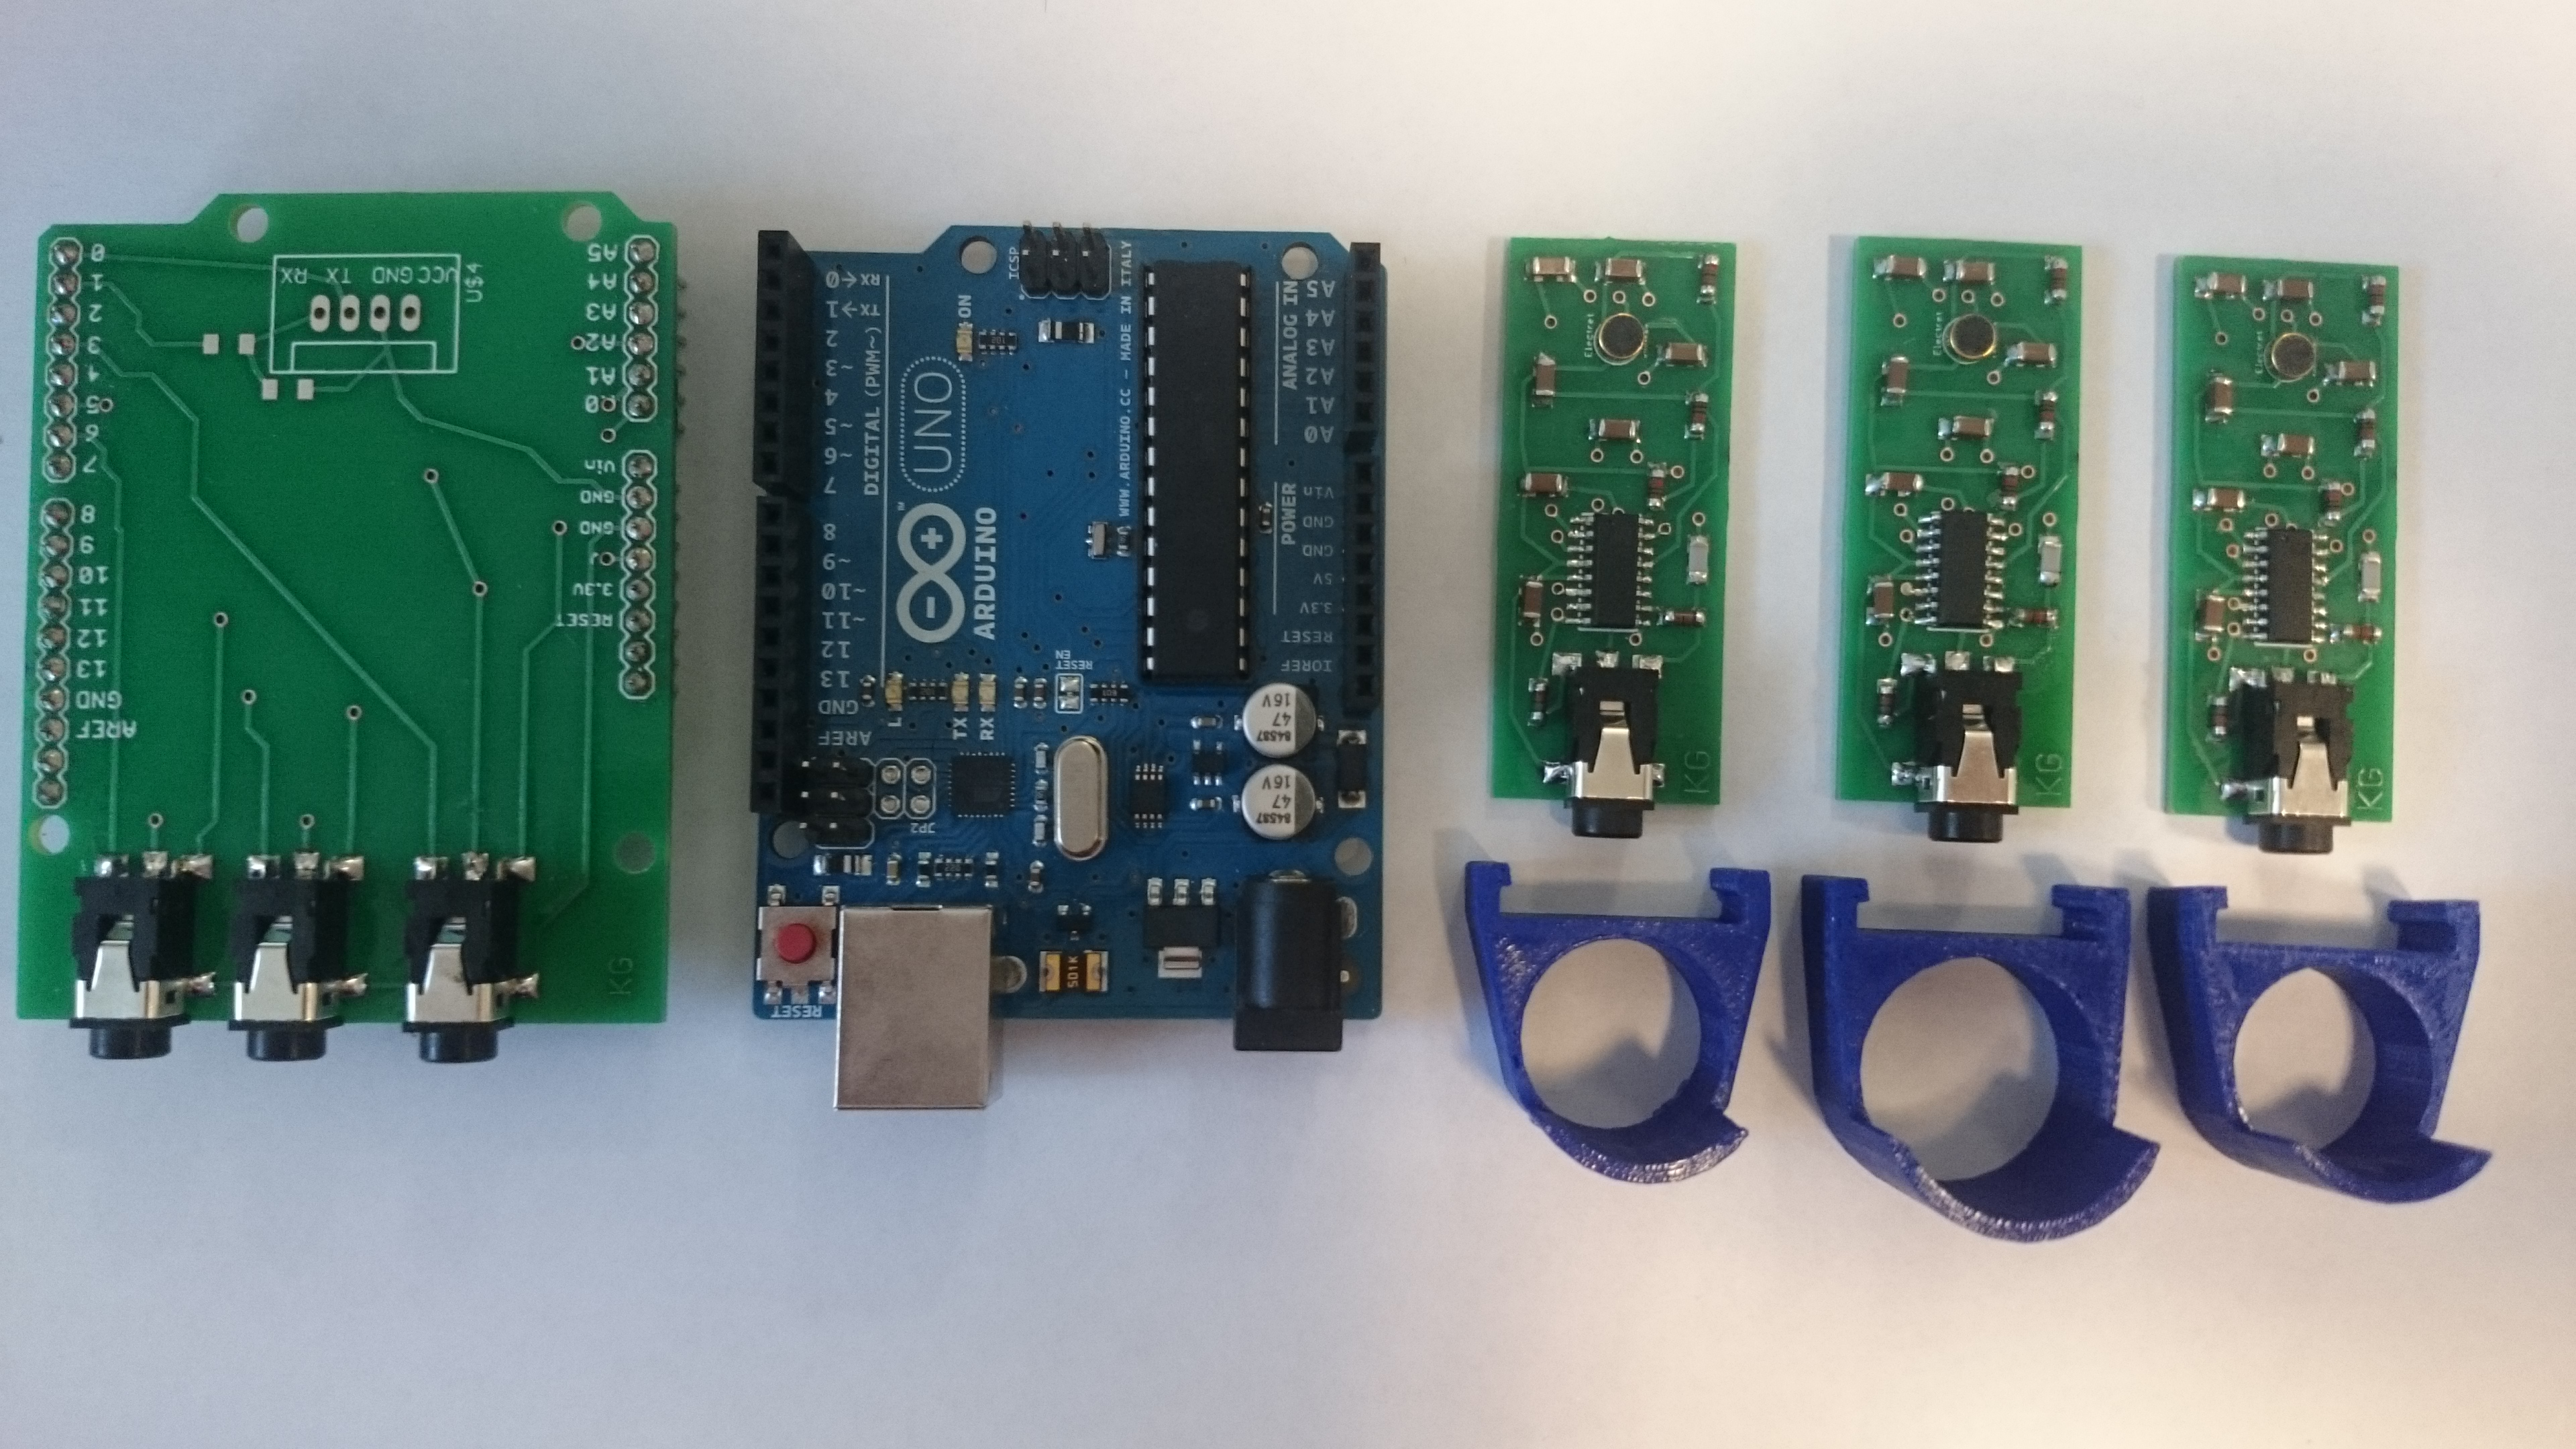
\includegraphics[scale=0.1]{Images/paws_full} 
\end{figure}

%%%%%%%%%%%%%%%%%%%%%%%%%%%%%%%%%%%%%%%%%%%%%

\vfill

\begin{tabular}{| l l}
Project Title & The development of a novel wearable musical instrument whose \\
& functionality is flexible and fully programmable through a \\ & simple interface \\
&\\
Student & K. K. GOHIL \\ 
CID & 00692607 \\ 
Course & EEE 4T \\ &\\
Supervisors & Prof Robert Spence, Dr Mark Witkowski \\ 
Second Marker & Dr Christos Papavassiliou 
\end{tabular}
%%%%%%%%%%%%%%%%%%%%%%%%%%%%%%%%%%%%%%%%%%%%%
\normalsize
\newpage
% !TEX root = /Users/kartikgohil/Documents/Imperial/Year4/Project/Docs/Final_Report/report_tex/main.tex
\thispagestyle{empty}

\begin{tabular}{|l}

\end{tabular}


%%%%%%%%%%%%%%%%%%%%%%%%%%%%%%%%%%%%%%%%%%%%%
\vspace{150 pt}
\begin{center}
\huge Programmable And Wearable Sound\\
\LARGE  (PAWS)\\
\bigskip
\LARGE by Kartiksinh Gohil

\end{center}

%%%%%%%%%%%%%%%%%%%%%%%%%%%%%%%%%%%%%%%%%%%%%
\vspace{100 pt}
\begin{center}
\textbf{Acknowledgements}\\
\textit{Special thanks to Imperial College Advanced Hackspace for their equipment,\\Vic Boddy for his assistance, and my supervisors for their advice.}\\

\end{center}
%%%%%%%%%%%%%%%%%%%%%%%%%%%%%%%%%%%%%%%%%%%%%

\vfill
\normalsize
%%%%%%%%%%%%%%%%%%%%%%%%%%%%%%%%%%%%%%%%%%%%%
\section*{Abstract} \label{Project Specification}

The aim of the project was the development of a novel wearable musical instrument whose functionality is flexible and fully programmable through a simple interface.

This report describes the design of a concept musical instrument in which the user wears sensors that can be programmed, through a software application, to generate sounds selected by that user. The concept is very general, and is illustrated by a 'demonstration-of-concept' prototype that has been developed and evaluated.  The prototype focuses on one representative function whereby the user, while wearing microphones on their fingers, can play a rhythm against an arbitrary surface: simultaneously, and in response, the software will play back previously selected sample sound files. For example, a user can play a full drum kit simply with their fingers, against a musical background of their choosing or as a solo performance.

Various mechanisms were developed to capture sound using a microphone, and to transmit this audio signal to a desktop application via an Arduino Uno. Python and C++ were both tested for creating the software interface, and the latter, using an audio processing library called JUCE, was finally selected for the later prototypes. A program was developed to read audio signals from a single Arduino Uno connected to three wearable circuit boards, each with their own microphone circuit, and was designed to control the sample sound file triggered by each. The user experience was a main consideration in the design of the instrument and the program included features such as a real-time waveform trace of the incoming audio signals to aid this. Further designs were subsequently looked into for improved technical implementation and greater functional creativity for the user.

%%%%%%%%%%%%%%%%%%%%%%%%%%%%%%%%%%%%%%%%%%%%%
\normalsize
\newpage


%%%%%%%%%%%%%%%%%%%%%%%%%%%%%%%%%%%%%%%%%%%%%

\tableofcontents
\vfill
\listoftables
\newpage
\listoffigures


\newpage
%%%%%%%%%%%%%%%%%%%%%%%%%%%%%%%%%%%%%%%%%%%%%
\section{Introduction} \label{Introduction}

The aim of this project is to design a modern musical instrument that gives a user the freedom to use their environment as part of their sound production process. I will be designing and implementing an instrument that consists of a microphone on a wearable circuit board that, when tapped against any surface, will trigger a sample sound file selected by the user through a software interface. In other words, the user will potentially be able to play an entire drum kit simply by tapping a rhythm with their fingers. The instrument will be limited to this functionality for this project but has a large future scope, in that it could integrate motion gesture control to allow a user to, for example, generate synthesised sounds and modify their amplitudes and pitches in real-time using spatial positioning, or to generate the sounds of guitar chords when mimicking the action of playing one (the air guitar concept). 

\begin{wrapfigure}{r}{0.4\textheight}
\centering
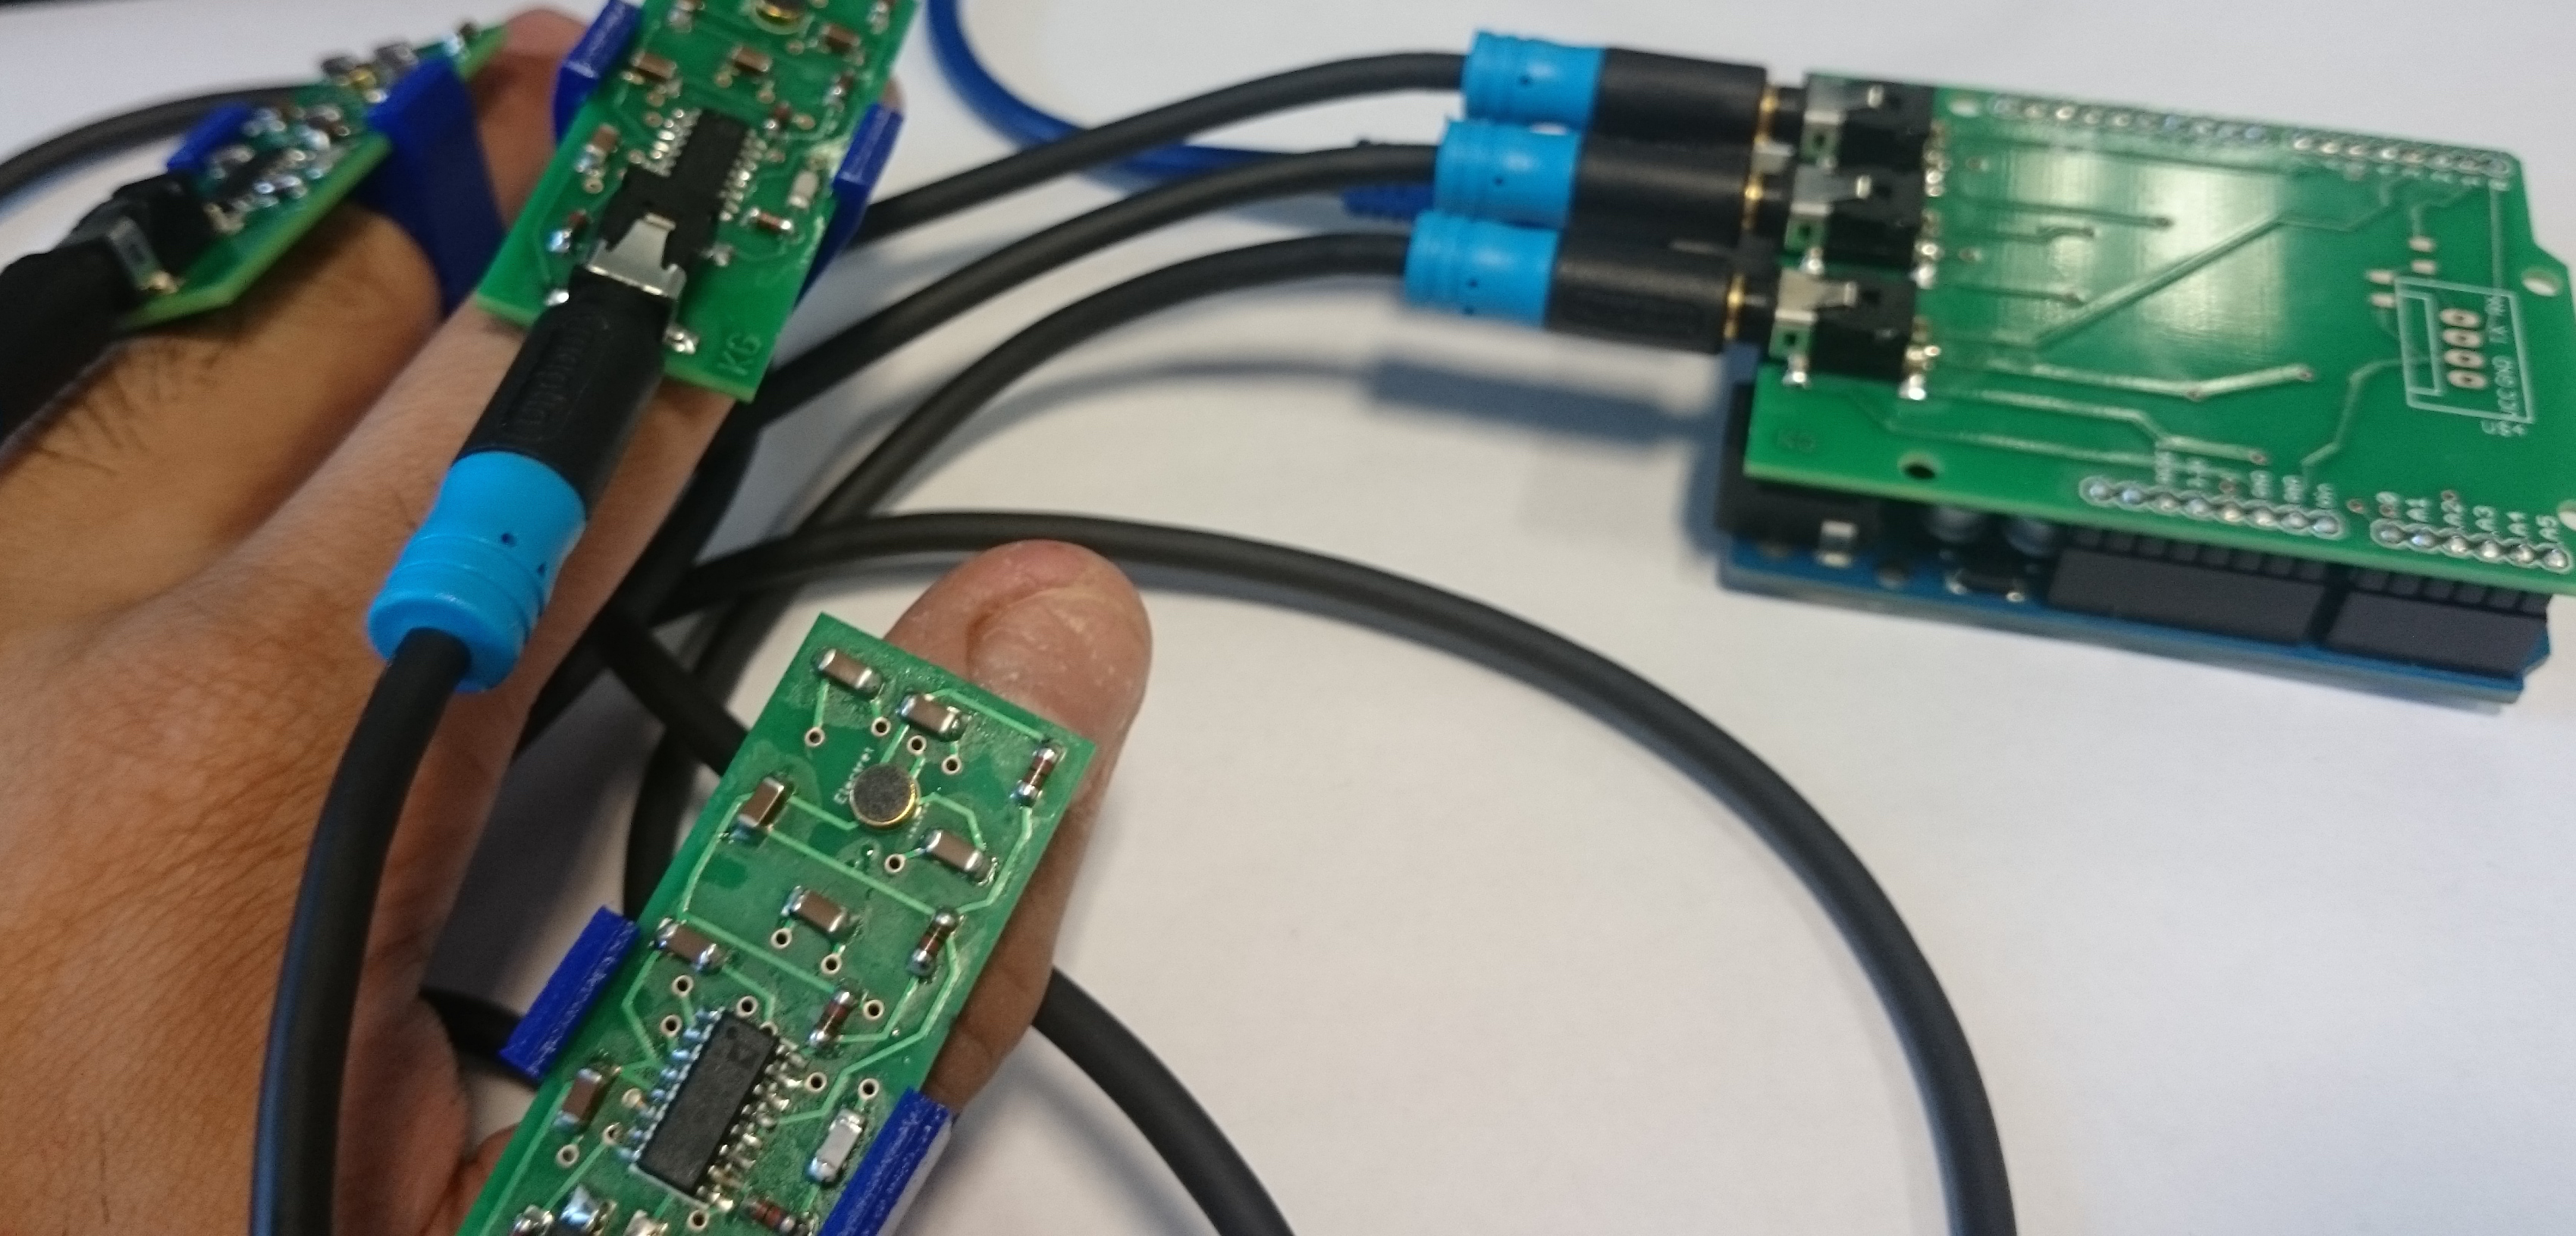
\includegraphics[scale=0.08]{Images/paws_0204}
\caption{Photograph of PAWS Prototype 0.2.04 in action}
\label{fig:paws_final}
\end{wrapfigure}

Section~\ref{Implementation} outlines the developments made during implementation. I started by using an Arduino Uno to interface my microphone with my computer's software application, which I initially began to code in Python. Through substantial testing and eventual failures, I switched to an audio library called JUCE in C++. I produced a user-friendly Graphical User Interface (GUI), with two functionalities: a 'Voice' mode to feed the microphone signal through to the computer's audio device, and a 'Sample' mode to trigger a user-selectable sample sound file in response to tapping the microphone. 

Throughout this project, I maintained the full scope of the product, detailed in Section~\ref{Product Concept} Product Concept, in mind. Despite focusing mostly on the 'Sample' function and ensuring that that was ready for a robust demonstration by the end of the project, consideration was always taken into the future development of the product, including the integration of accelerometers for motion control, despite not having had the chance to test them. 

The most difficult part of this project was designing a fast and reliable method of data transmission, from sampling the microphone signal on the Arduino side, to transmitting it via USB to the computer, processing the signal accordingly, and throwing the relevant data to the computer's audio device. Dealing with what was effectively a multirate system, where the sample rates were variable at each stage of data capture or transmission, was challenging but developing a strong data structure for each of these components and optimising the speeds of data transmission and processing at each stage inevitably led to an overall successful system. 

This report begins with some research into the current market for wearable technologies, especially in the field of music production. Section~\ref{Product Concept} Product Concept involves the design of an idea for a musical instrument to fit the original brief: \textit{'The development and evaluation of a novel and unusual musical instrument to be constructed using a 3D printer'}. Section~\ref{Requirements} analyses the requirements the designed product will have to meet, and the following sections detail the design of the product and initial testing of my sample triggering theories and key components such as an Arduino Uno microprocessor. Section~\ref{Implementation} Product Implementation provides a discussion on the development of my various prototypes from the design stage to a working demonstrable product. Subsequently, I evaluate the final prototype and the progress of my project and also detail further developments to be made if the project were to be continued. Section~\ref{Finances} Finances provides a summary of the costs incurred in developing each prototype and the projected costs of future designs, and Section~\ref{User Manual} provides a User Manual on using my final prototype. Appendices have also included at the end with supporting diagrams and schematics. 


\newpage
%%%%%%%%%%%%%%%%%%%%%%%%%%%%%%%%%%%%%%%%%%%%%
\section{Background} 

This section summarises research of the current musical instrument market, specifically in wearable and motion-control technologies, and hence outlines a concept for a new instrument.

\subsection{Market Research} \label{Background}
This project's original brief was \textit{'The development and evaluation of a novel and unusual musical instrument to be constructed using a 3D printer'}, which was fairly open-ended, relying more on a creative user-oriented approach rather than the usual best-fit engineering solution. This section outlines the current state of the musical instrument market and a few products I researched and analysed in order to design my own concept.

The definition of a 'musical instrument' has evolved drastically over the years, ranging from traditional acoustic instruments (\textit{piano, violin}) to electrical (\textit{guitars, keyboards}), electronic (\textit{synthesisers, Theremin}), and even to virtual instruments that exist purely as software models in computer-based audio production tools.

With the initial introduction of electronic instruments, musicians became confined to button-based keyboards and drum machines, and later to point-and-click software on computers. 
It is only now that we are beginning to see computer vision and wearable technologies penetrating the market, giving way to innovative products such as the \emph{Mi.Mu}\textsuperscript{\cite{mimu}} gloves and \emph{DrumPants}\textsuperscript{\cite{drumpants}}. The idea of capturing motion through worn sensors or distant cameras allows users to integrate their bodies with electronic systems. Musicians can make sweeping gestures to produce and control sounds, much like was traditionally done with mechanical instruments. 

\begin{wrapfigure}[16]{r}{0.37\textwidth}
\centering
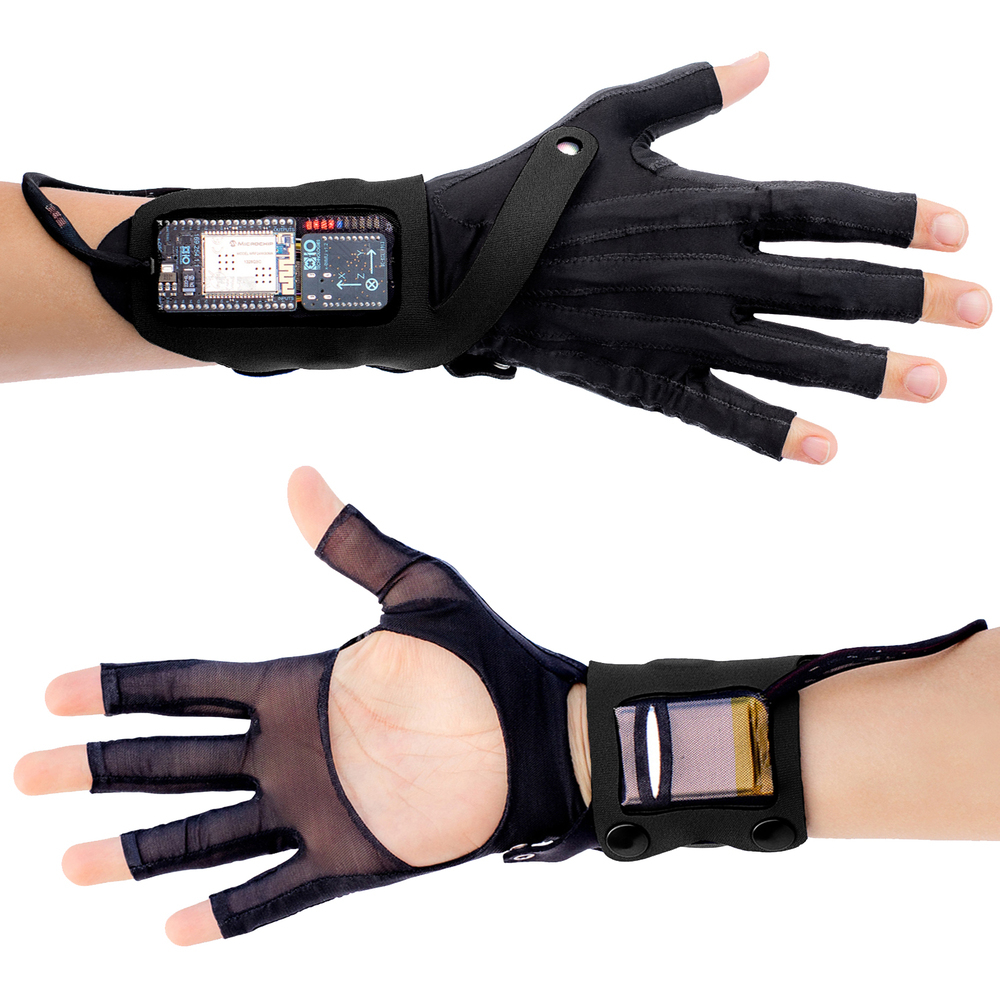
\includegraphics[scale=0.5]{Images/MiMuGloves}
\caption{Mi.Mu Gloves\textsuperscript{\cite{mimugloves}}}
\label{fig:mimugloves}
\end{wrapfigure}

New technologies have allowed the modern musician to let the motion of their body contribute to their overall sound but they still seem to be fairly restrictive. The Mi.Mu gloves, as shown in Figure~\ref{fig:mimugloves}, allow users to generate music simply by moving their hands. The gloves feature motion sensors and a battery-powered microcontroller to transmit generated signals as MIDI data to control audio sequences pre-programmed on a software application. For example, a user could emulate playing a drum kit with their hands and the gloves would send MIDI signals to a digital audio workstation (DAW) to produce the correct sounds in response to the user's 'air-drumming'. The gloves can also be used to control functions on sound, such as altering amplitude, filtering and even adding effects like Reverb, all through a pre-determined hand motion. This technology, however, is incredibly expensive. Provisionally selling at nearly \pounds 5000\textsuperscript{\cite{mimugloves}}, these gloves are not accessible to the average person. The fact that these gloves require supplementary software tools to interact with confines the user to a particular physical workspace, be it a studio or a live stage, which requires an extraordinary amount of setting up and calibration before use. 


\begin{wrapfigure}[12]{r}{0.6\textwidth}
\centering
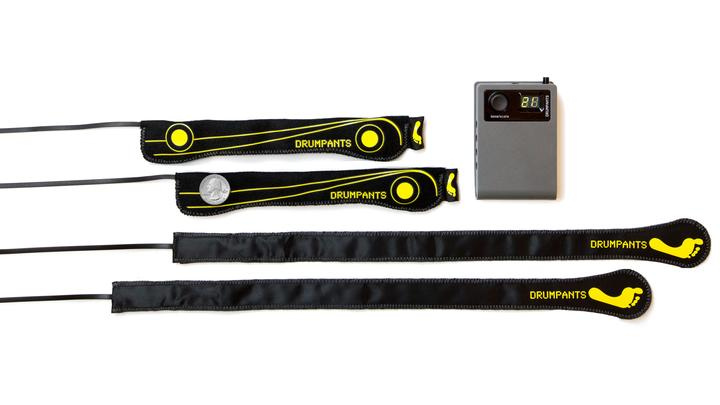
\includegraphics[scale=0.35]{Images/drumpantsbasic}
\caption{DrumPants Basic Kit\textsuperscript{\cite{drumpantsprice}}}
\label{fig:drumpants}
\end{wrapfigure}

DrumPants is another product that utilises wearable sensors to control sounds. The instrument, shown in Figure~\ref{fig:drumpants}, uses sensor strips that attach to your clothes and connect wirelessly to a central controller. The strips contain pressure sensors that, when hit, send MIDI data to the controller, which can be programmed by the user to play any virtual sound in response, such as a drum kit or a piano. This controller can output audio directly to a speaker or can send the raw MIDI data to a compatible computer program. Currently on pre-order from \$129.99\textsuperscript{\cite{drumpantsprice}}, this instrument allows the user to program each sensor to play any pre-recorded sample sound, and is also being marketed to be able to remotely control video games. The functionality, however, is limited to contact via pressure, and slightly malforms the user's experience by again restricting them to a particular physical area. Even though this physical workspace, or the area where the sensor is located, is movable between instances of use, it still limits the musician's ability to improvise and requires an inordinate amount of setup time before playing can commence. 

\begin{wrapfigure}{r}{0.4\textwidth}
\centering
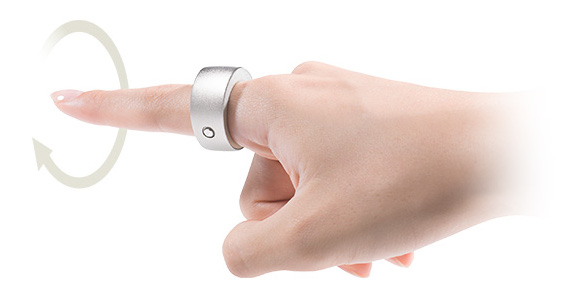
\includegraphics[scale=0.3]{Images/gesturering}
\caption{Ring by Logbar Inc.\textsuperscript{\cite{gesturering}}}
\label{fig:gesturering}
\end{wrapfigure}

A third product, not specifically designed for music but relevant nonetheless, is the \emph{Ring}\textsuperscript{\cite{gesturering}} by Logbar Inc. The Ring has the capability of controlling any web-linked interface through an Android or iOS App using gestures. It is designed for the user to assign gestures to specific features, from controlling music play-out on a smartphone to opening a set of shower curtains (provided they have internet connectivity). The idea behind the Ring is that it allows a user to directly interact with the world around them through a portable wearable sensor with apparently no physical limitations. The concept of this device, in its functionality and freedom of use, would greatly enhance a musician's creativity if applied to the world of sound.

Based on these products, I produced a new musical instrument that heads in the direction of user-programmable electronics, which is portable and not restricted to a physical workspace in the way that most other motion-based products are (especially those related to computer-vision). The musical instrument should allow the user to define the manner in which they wish to produce sounds and should allow them to use the range of their entire bodies in the process without introducing any physical or mental limitations. 

%%%%%%%%%%%%%%%%%%%%%%%%%%%%%%%%%%%%%%%%%%%%%
\subsection{Product Concept for a new Instrument} \label{Product Concept}

\begin{wrapfigure}[14]{r}{0.5\textwidth}
\centering
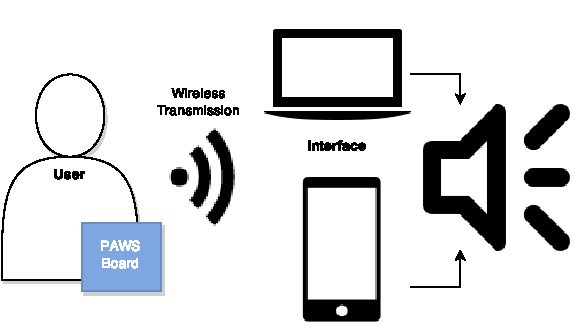
\includegraphics[scale=0.8]{Images/UserLevelDia}
\caption{PAWS - Concept User Level Diagram}
\label{fig:userlvl}
\end{wrapfigure}

The musical instrument I designed features the concept of Programmable And Wearable Sensors (PAWS). The instrument consists of a hardware aspect, i.e. wearable sensors, and a software aspect to control the functionality of these circuit boards. The wearable sensors should be small and light to increase the adaptability of their use as well as removing the restrictions of a fixed physical environment. 

A PAWS Board, made up of audio and motion sensors, has the ability to be worn by the user on any part of their body. To achieve this, plastic housings will be 3D Printed in the shape of clips or rings or wristbands for the user to wear, which PAWS Boards can then be attached to. The ability to allow the user to print their own housings is significant and will allow users in the near future to interact more closely with PAWS Boards. These worn PAWS Boards can then be programmed by the user through a software Interface, hosted on either a computer or a smartphone, to complete any given task. The PAWS Board's generated audio data will be transmitted back to the Interface for processing and storage. Figure~\ref{fig:userlvl} shows a user-level diagram of a PAWS Board sending information wirelessly to an Interface and consequently producing audio.

The aim of the PAWS instrument is to be fully programmable and flexible in functionality. The user should be able to perform functions such as recording their voice, emulating a real live drum kit, mapping a tempo, and even harmonising their singing with virtual instruments, all by programming the sensors in various ways. The user will have the ability to wear as many PAWS Boards as they like and program each one separately. Figure~\ref{fig:conceptphoneinterface} shows a concept sketch of the Interface on a smartphone. This mockup shows how the user would go about connecting to PAWS Boards and programming them individually. 

\begin{wrapfigure}[26]{r}{0.37\textheight}
\centering
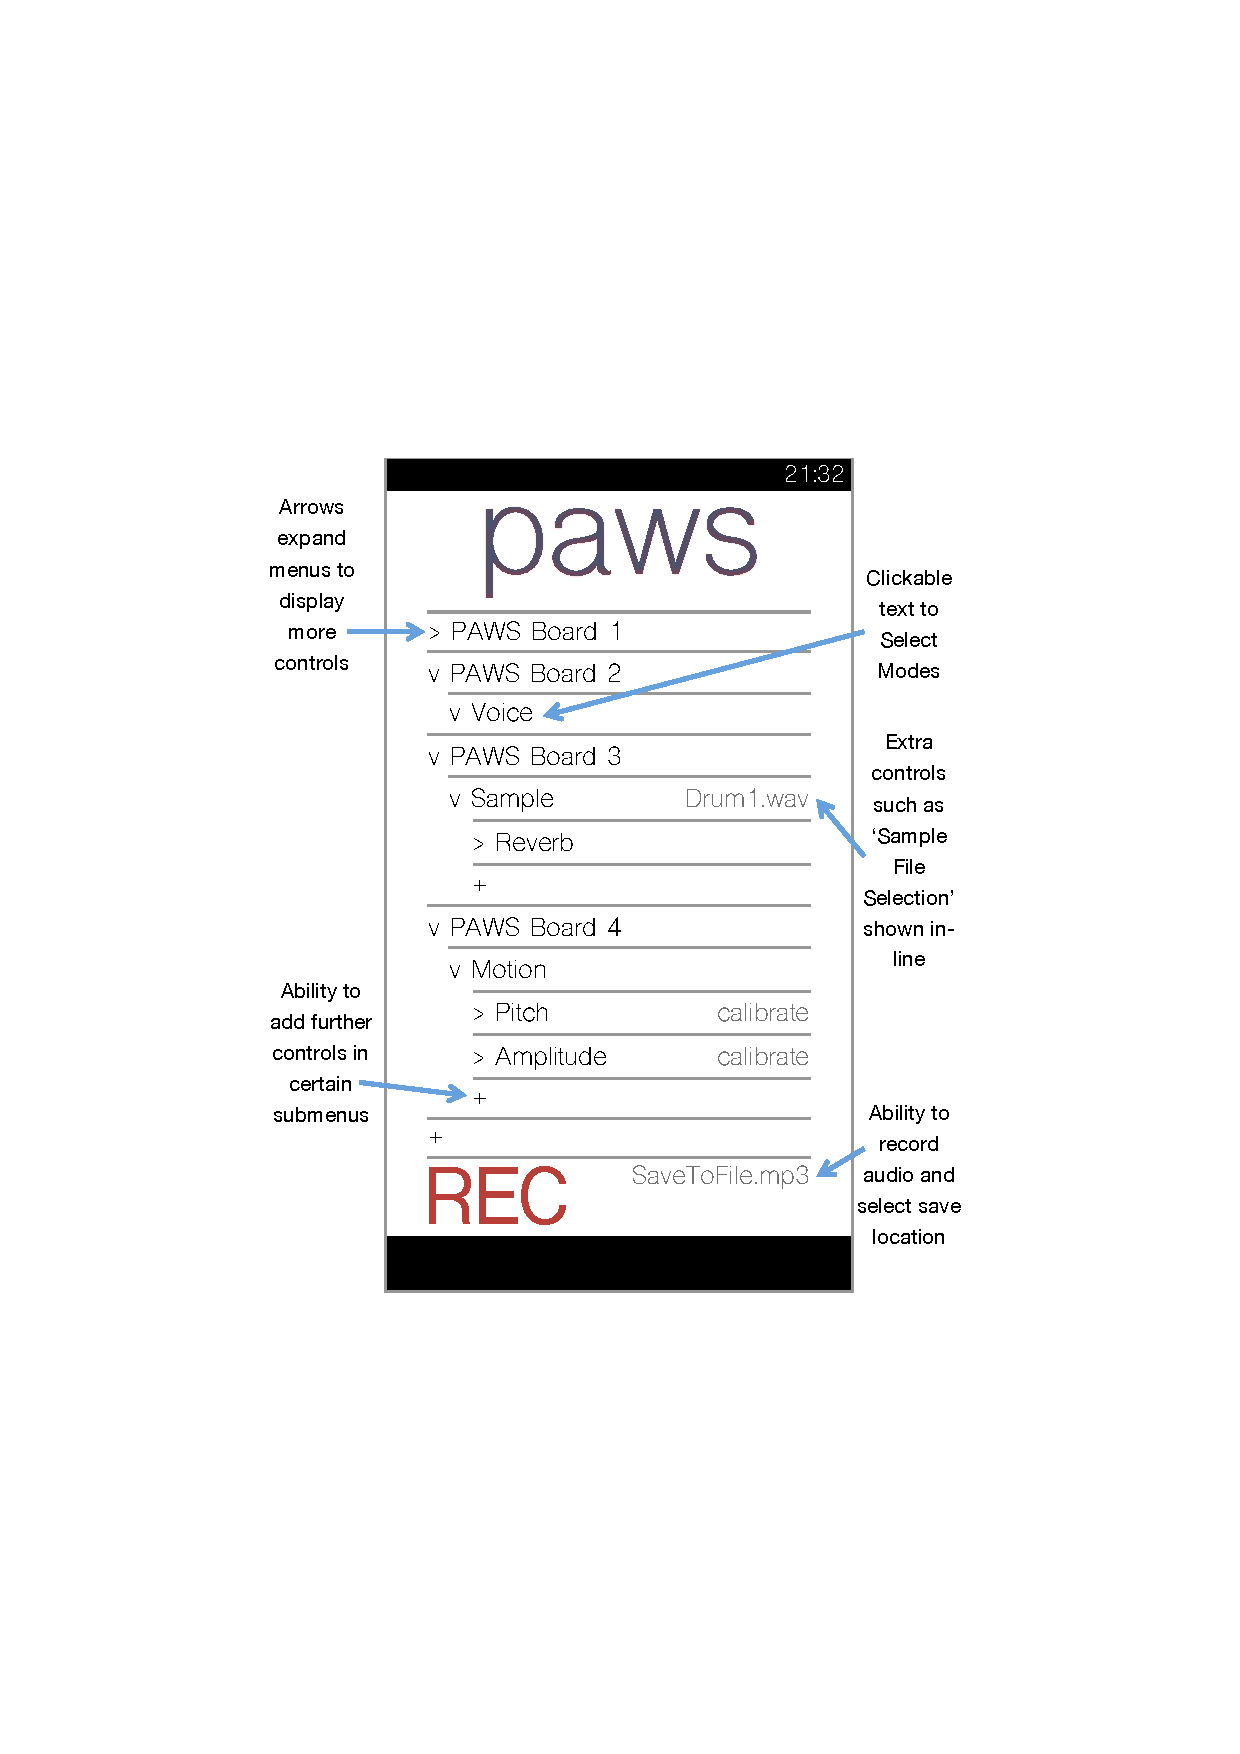
\includegraphics[scale=0.7]{Images/conceptphoneinterface_annotated}
\caption{PAWS - Concept Design for a smartphone-based Interface}
\label{fig:conceptphoneinterface}
\end{wrapfigure}

\newpage
This sketch shows three modes of functionality: 'Voice', 'Sample' and 'Motion'. The 'Voice' mode simply captures audio from a PAWS Board and outputs it directly, allowing the user to record themselves or other audio. The 'Sample' mode gives the user the ability to trigger sample sound files based on percussive motion. For example, if the user was wearing PAWS Boards on their fingers and they began to tap a rhythm on a surface, the Interface would play back a sample sound file (for example, of a kick drum) in response. Thus, the user would be able to emulate playing a full drum kit simply by hitting an arbitrary surface. The third 'Motion' mode is by far the most flexible in that it allows the user to map any motion gesture to a particular function. By calibrating motions such as sweeping gestures or pinching their fingers, the user will be able to either synthesise tones with control over pitch and amplitude, or control the parameters of other PAWS Boards such as modulation, filter cutoff frequencies, etc. Figure~\ref{fig:conceptsketch} shows concept sketches for how PAWS Boards could be used in the 'Sample' and 'Motion' modes. 


\begin{figure}[H]
\centering
\subfloat[PAWS Board: Motion Function]{
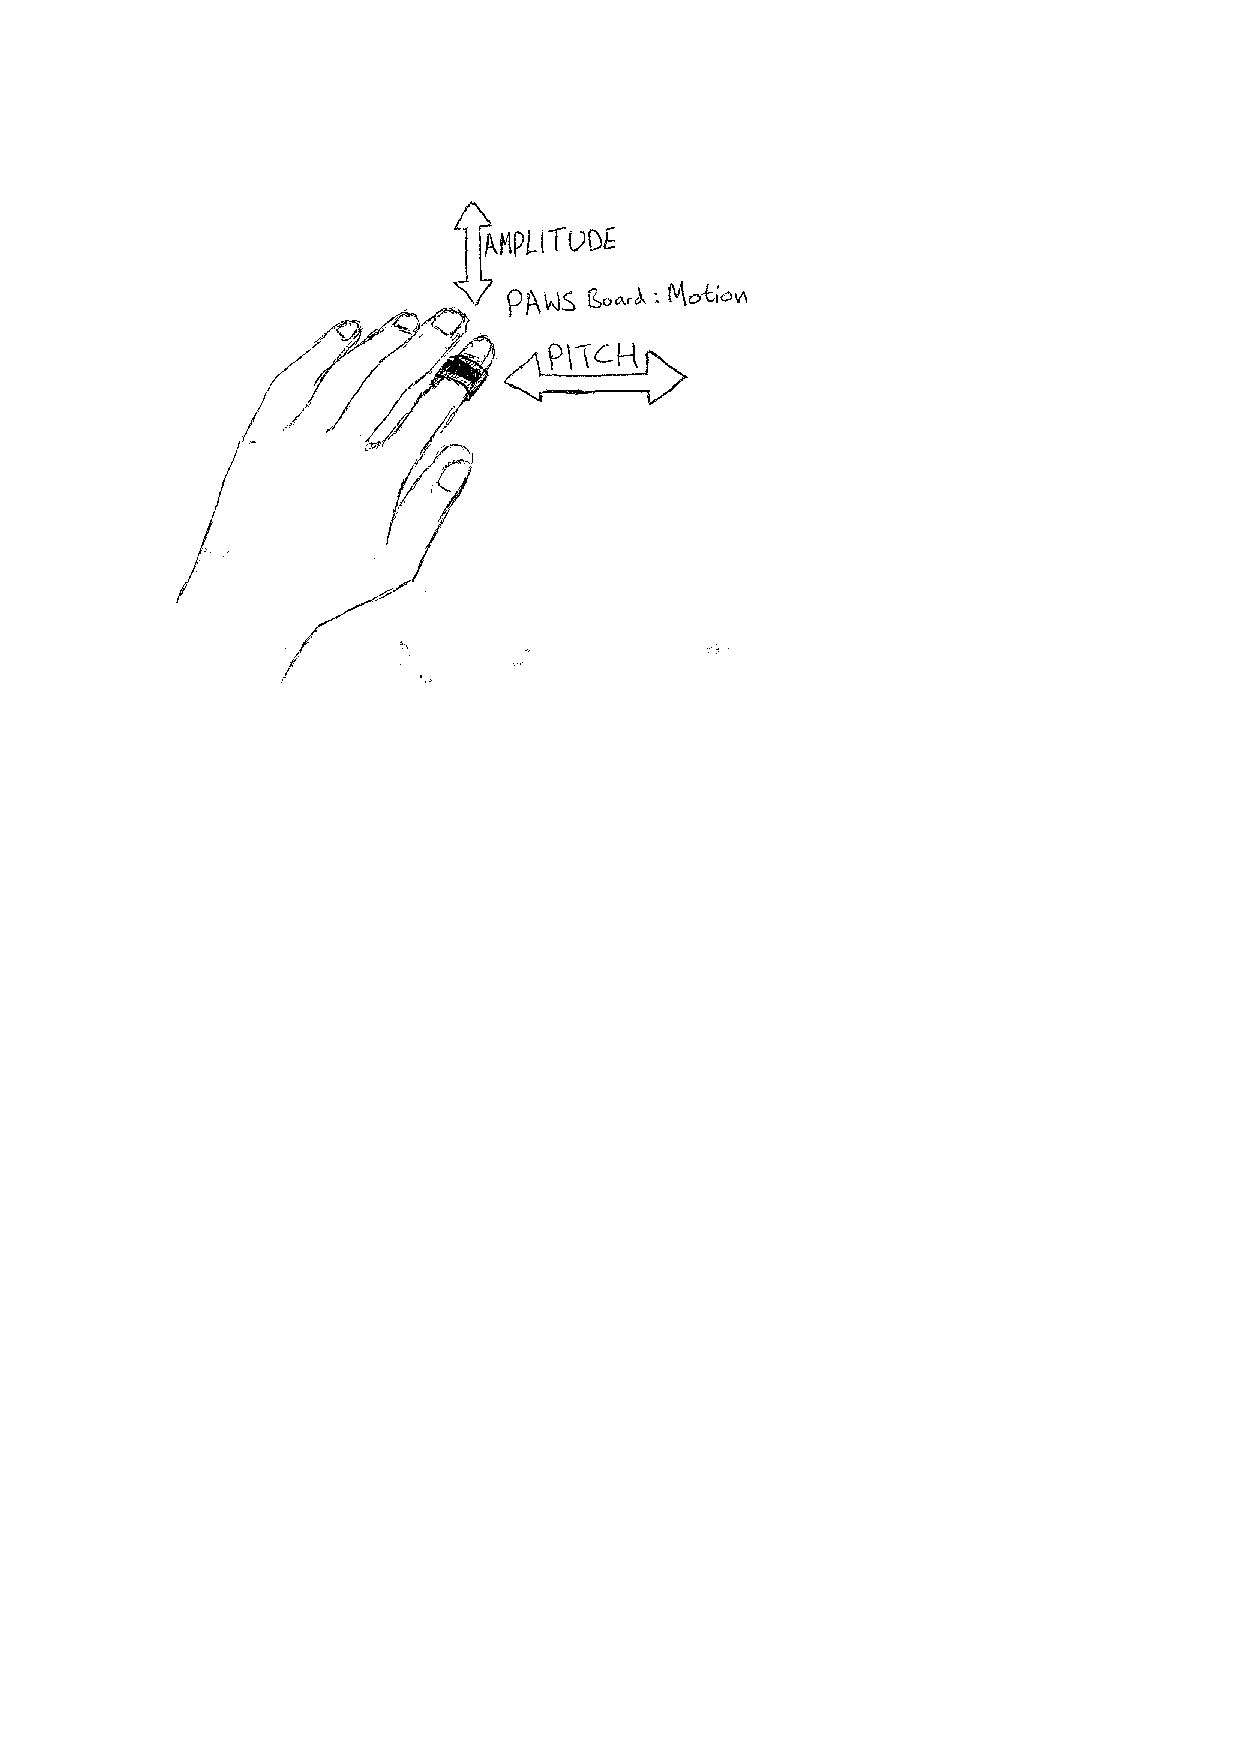
\includegraphics[scale=0.7]{Images/conceptsketchesleft}
\label{fig:conceptsketchleft}
}
\subfloat[PAWS Board: Sample Function]{
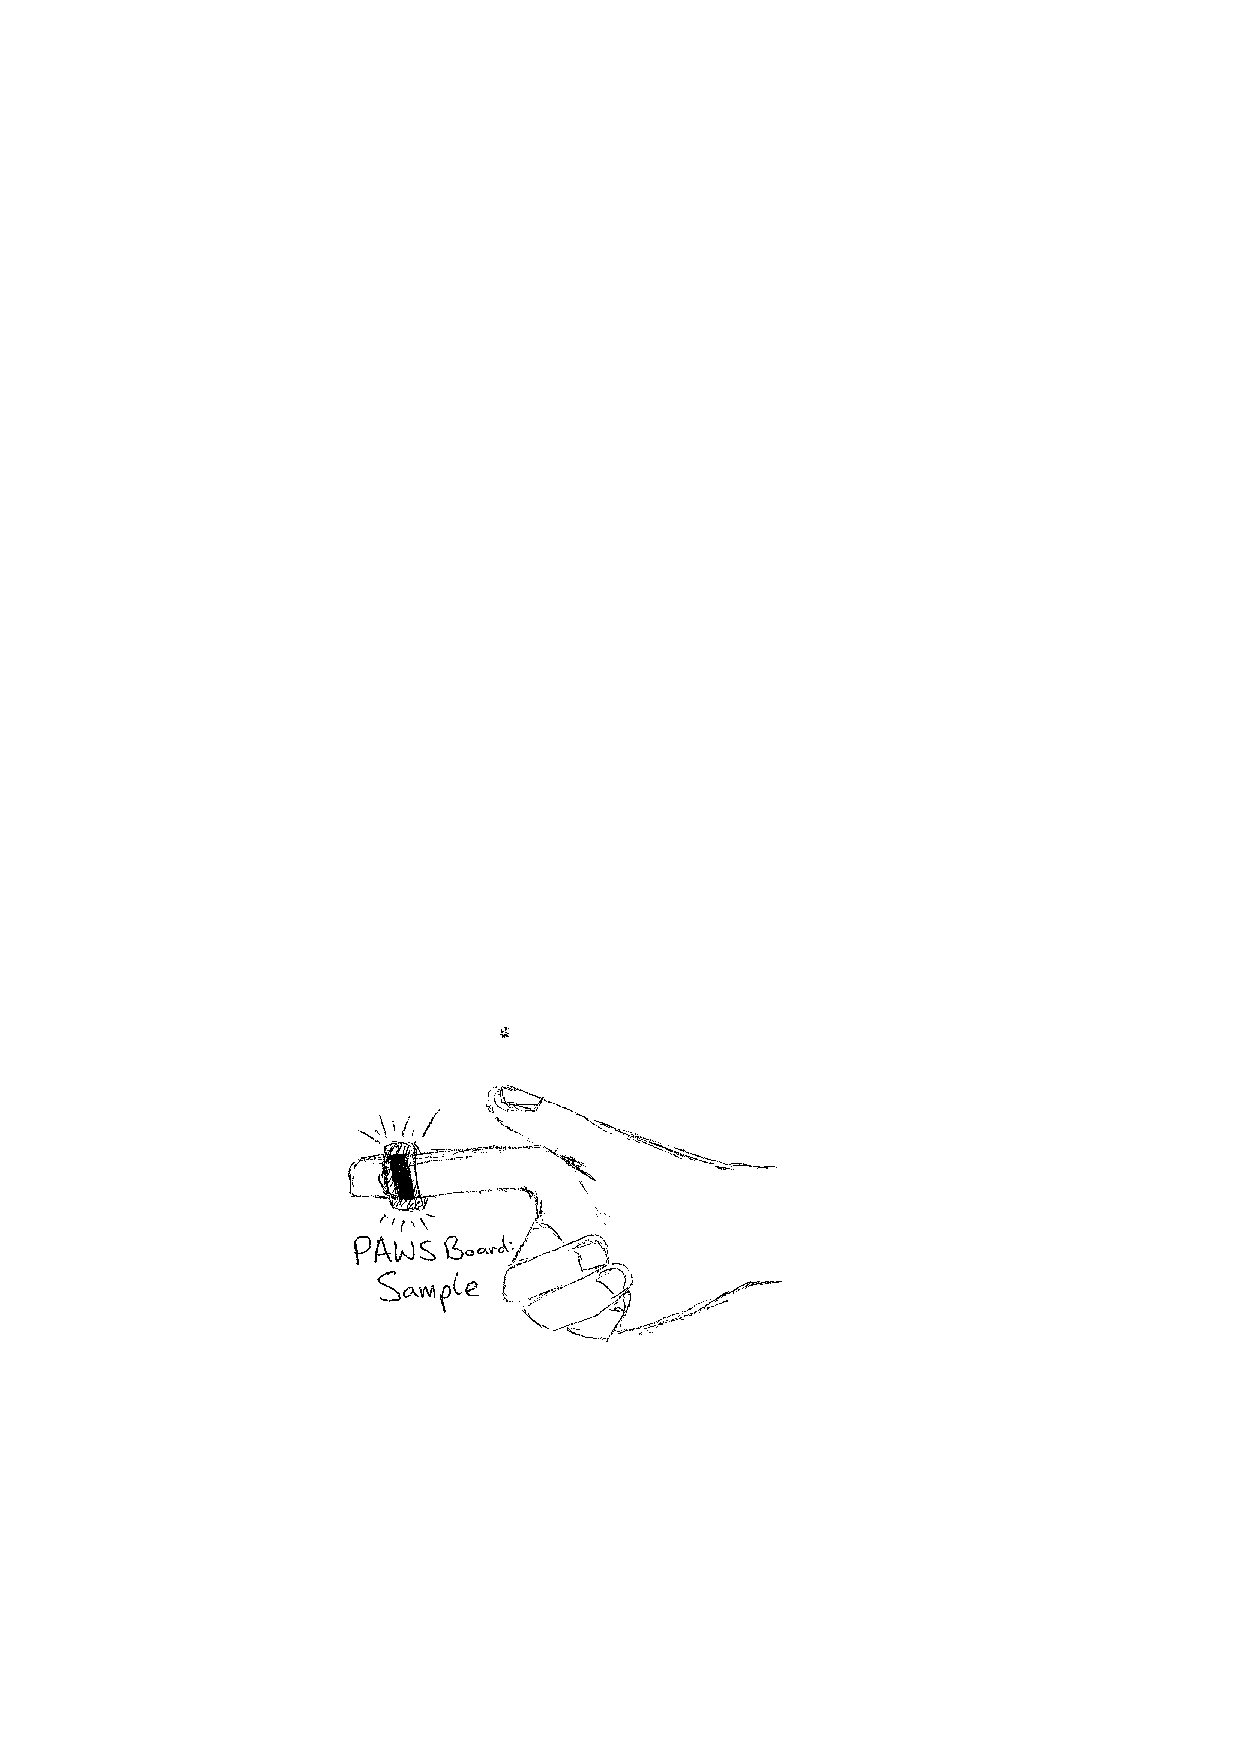
\includegraphics[scale=0.7]{Images/conceptsketchesright}
\label{fig:conceptsketchright}
}
\caption{PAWS - Concept Sketch of usage}
\label{fig:conceptsketch}
\end{figure}

Further designs for the PAWS Board involve allowing a musician to set a particular tempo by tapping their feet (with a PAWS Board attached), which could subsequently aim to quantise any other sounds that they produce, thus improving the playback quality. The 'Sample' function could also be used to let a musician harmonise with themselves. For example, if they were singing into one PAWS Board and tapped another against a surface, as if playing a piano, the instrument could trigger a piano sample at the same pitch as their vocal melody. Multiple PAWS Boards for sample triggering could be used to allow a musician to play entire chords in harmony with their voice. The possibilities for the PAWS instrument are endless as it is all about giving a user the ability to make sounds as they wish, thereby removing all limitations on their creativity.

\newpage
%%%%%%%%%%%%%%%%%%%%%%%%%%%%%%%%%%%%%%%%%%%%%
\section{Product Design} \label{Concept Design}

This section outlines the design of the PAWS instrument. Section~\ref{System Design} outlines the design of the overall system with its various conceptualised functionalities, while Section~\ref{Implementation Design} talks about the methods in which the system will be implemented for the purposes of this project. 

\subsection{System Design for Concept}\label{System Design}

\begin{wrapfigure}{r}{0.3\textheight}
\centering
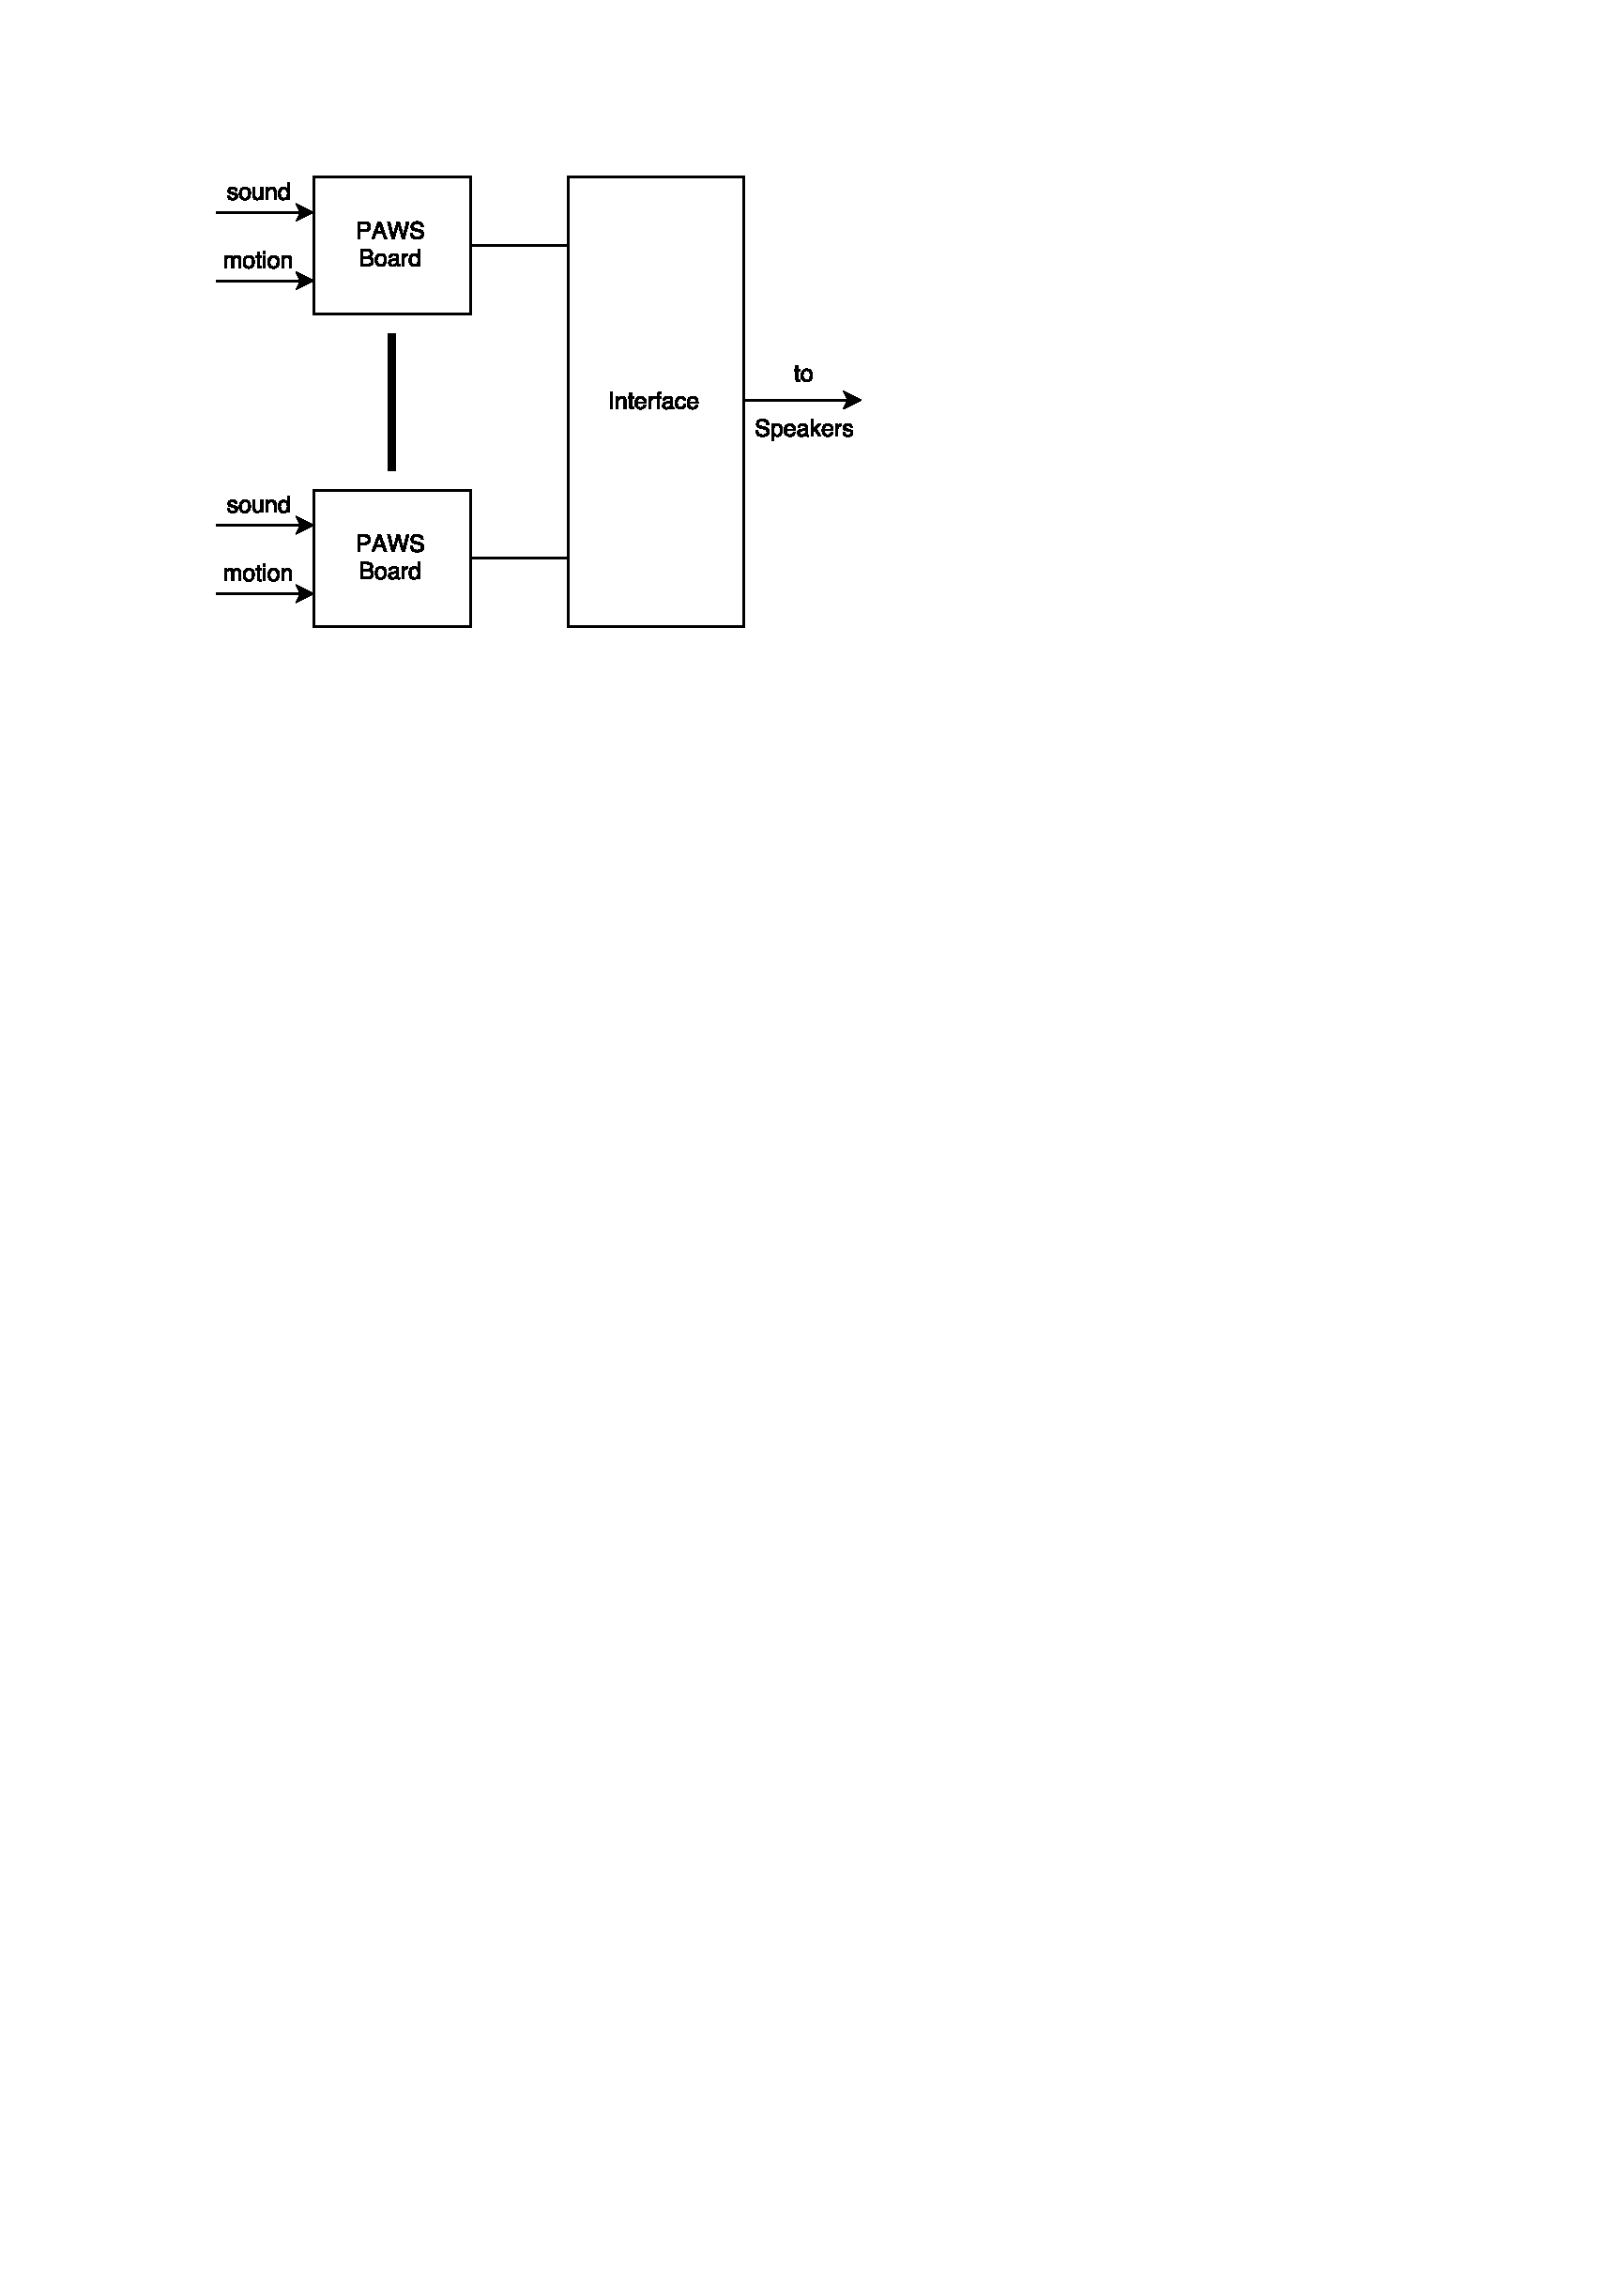
\includegraphics[scale=0.6]{Images/SystemLevelHi}
\caption{System Design for Concept Product - High Level}
\label{fig:syslvlhi}
\end{wrapfigure}

Figure~\ref{fig:syslvlhi} shows the high-level system design of the instrument, where multiple hardware PAWS Boards, each with the ability to capture sound and motion data, connect to a central interface which processes the incoming data and produces an audio output. 

Figure~\ref{fig:syslvllo} gives a more detailed view of the processes involved inside the PAWS Boards and the Interface. A PAWS Board features microphones for capturing sound and accelerometers for capturing motion artefacts. The signals are stored temporarily before being transmitted to the central Interface. Some processing of the audio signal can be accomplished on the PAWS Board itself but has deliberately been left open-ended in the diagram for development as required. The Interface is designed to receive signals from a multitude of PAWS Boards and process them according to user programming. The diagram shows the processing procedure for a single connected Board. 

The user must firstly select the mode for the connected Board to operate in. The 'Voice' mode, if selected, simply routes the sound data to the output. The 'Sample' function allows the user to select a sample sound file and then processes the input motion data in order to trigger this sample sound in response to the user's 'tapping' actions. The 'Motion' mode allows the user to calibrate a particular gesture (such as sweeping a PAWS Board horizontally through the air) and assign it to change a particular modification parameter. For example, the selected parameter could be the global amplitude of the output audio, and the motion gesture would provide a continuous scale to change the amplitude level. 

%\newpage
\begin{figure}[H]
\centering
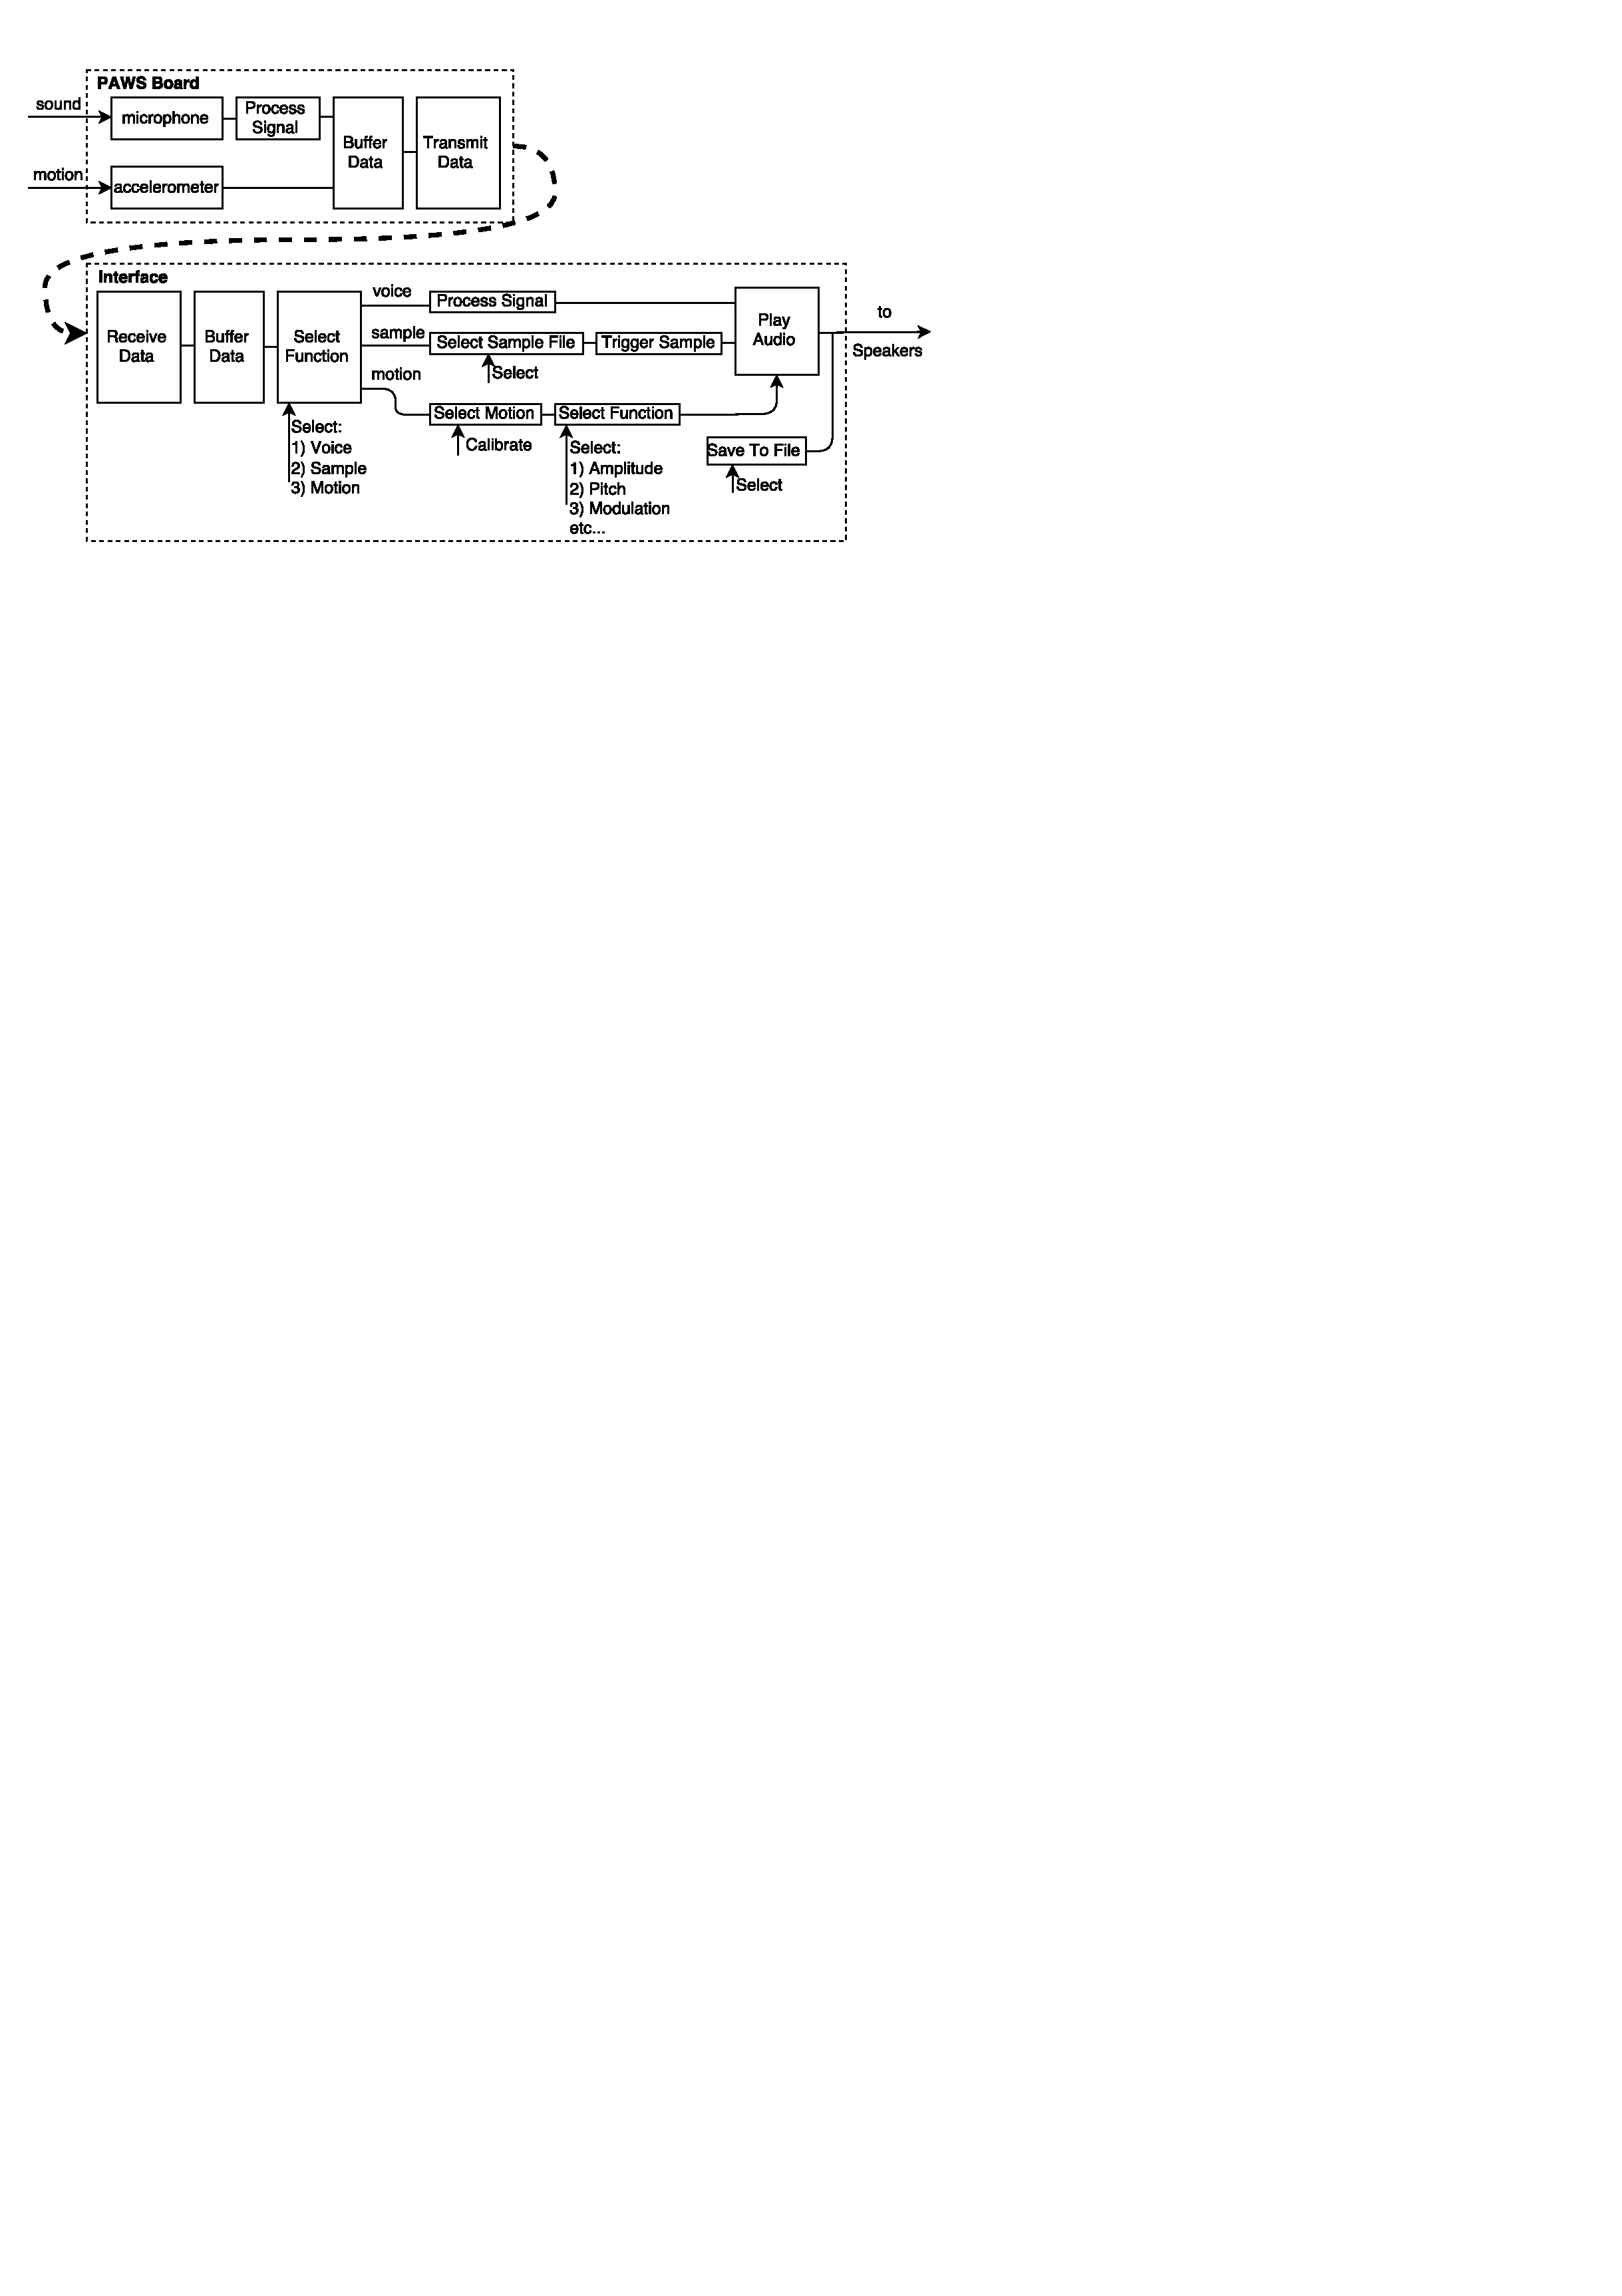
\includegraphics[scale=0.65]{Images/SystemLevelLo}
\caption{System Design for Concept Product - Low Level}
\label{fig:syslvllo}
\end{figure}

In this Concept System Design, the 'Motion' function serves to control particular parameters of the global audio output rather than to synthesise its own tones, in which case the \textit{Select Function} process would instantiate a tone generator controlled by the input motion data and feed the output sound to the final \textit{Play Audio} process. The Interface also allows the user to save the produced audio to a file, and its save location can be selected by the user. 


\subsection{System Design for Implementation}\label{Implementation Design}

For implementation purposes, the PAWS Board concept design was separated into two subsystems: a microphone circuit for capturing audio, and a microprocessor circuit to convert the analogue signal to digital and transmit it to the Interface. The Interface was designed to be implemented as a computer application (specifically built for Mac OS X) for proof-of-concept. The fact that the Interface was not designed as a smartphone application severely hampered the concept of the instrument's portability, but it was decided that implementing the entire instrument in a rough manner would prove to be better than designing one particular element incredibly well. 

All motion features and accelerometer circuitry were not included in the implementation until the microphone circuitry was deemed to be working robustly. The 'Sample' function was designed to work by detecting 'tapping' in the audio signal so that the instrument would offer two fully featured modes of functionality. 

\begin{figure}[H]
\centering
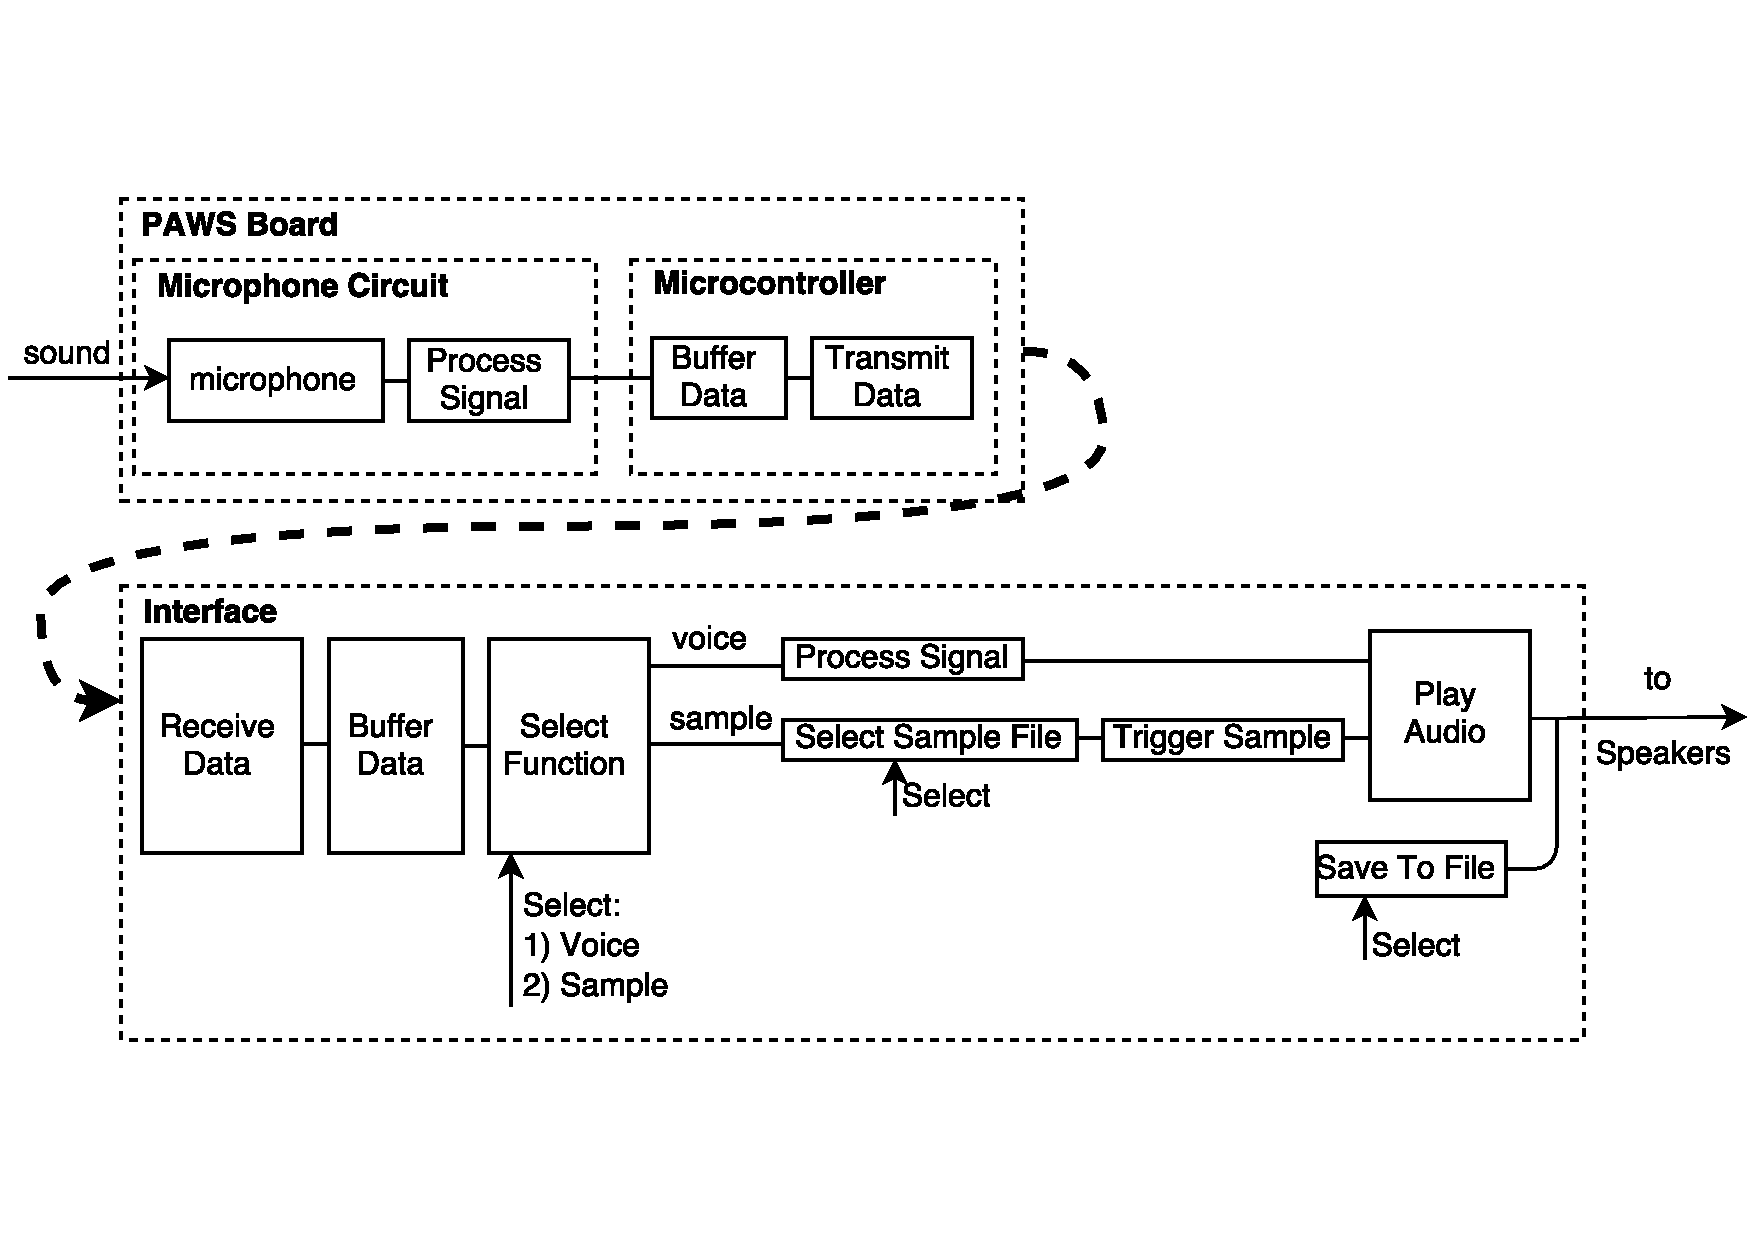
\includegraphics[scale=0.5]{Images/SystemLevelImp2}
\caption{System Design for Implementation of Product}
\label{fig:syslvl_imp}
\end{figure}

Figure~\ref{fig:syslvl_imp} shows a system design for implementing a PAWS Board and Interface. The PAWS Board hardware was conceptually defined as being portable, easily attachable to 3D printed wearable housings, and small enough to be placed anywhere on the body. For the implementation, the microphone circuitry was designed and tested using Breadboard and Veroboard, and was eventually printed onto circuit boards with fairly large components for ease of testing. The Interface was designed using \textit{Python}, which is simple to program but overall fairly bulky in terms of processing time, and later in \textit{C++} for a much lower-level (and therefore more efficient) implementation of signal manipulation techniques. All of these design changes meant that the implemented prototypes did not meet some of the ideologies behind the instrument: of being portable and physically non-restrictive, but the design was able to prove the flexibility of the instrument in terms of how the user could program each Board to perform a given function.

The implementable design was therefore not focussed on building perfect sensor arrays with minimum latency, or on developing new signal processing technologies, but rather on conglomerating the various existing ideas on the market into a single instrument that could be used by musicians and non-musicians alike to accomplish any task. The key features of this instrument to be demonstrated through prototyping will be flexibility and simplicity of use.


\newpage
%%%%%%%%%%%%%%%%%%%%%%%%%%%%%%%%%%%%%%%%%%%%%
\section{Product Requirements} \label{Requirements}

This section explores what will be required of the implemented product and details the necessary specifications to evaluate each prototype against. The plan to evaluate the success of the musical instrument, and therefore of the project, revolves around its ability to produce whatever sounds the user wishes of it and to give the user an easy and intuitive experience in doing so. The requirements of the instrument specified in Section~\ref{Implementation Design} System Design for Implementation have been listed in Table~\ref{tab:specifications}. Features for future concepts have also been included to ensure that all implementations of the instrument head in the direction of the overall concept.

\begin{table}[H]
\centering
\begin{tabular}{|l}
\textit{The PAWS Board}\\ \hline \hline
Can it capture audio? \\
Can it modify the amplitude of the audio signal?\\
Can it modify the frequency content (filter) the audio signal?\\
Can it capture motion? \\
Can it connect to the Interface? \\
Can it send captured data to the Interface via wired transmission?\\
Can it send captured data to the Interface via wireless transmission?\\
Is it wearable through 3D printed attachments? \\
Is it comfortable to wear?\\
Can it be switched on and off?\\
Can it remind the user of its functionality?\\
Can it be carried in a pocket or bag? \\
\hline \hline
\textit{The Interface} \\ \hline \hline
Is the Interface available on a computer? \\
Is the Interface available on a smartphone? \\
Can it connect to PAWS Boards? \\
Can it read data sent by the connected PAWS Boards?\\
Can the user control the function of every connected PAWS Board? \\
Can it modify the amplitude of the audio signal from each PAWS Board?\\
Can it modify the frequency content (filter) the audio signal from each PAWS Board?\\
Can it map motion gestures to control parameters?\\
Can it open and play sample sound files?\\
Can it trigger sample sound files from PAWS Board data?\\
Can it output the generated audio to the output audio device? \\
Can it save the output audio to file?\\
\end{tabular}
\caption{List of Specifications for Evaluation of Product}
\label{tab:specifications}
\end{table}

A more open-ended set of questions is shown in Table~\ref{tab:criteria}, which can be answered qualitatively to enable a discussion on the objectives a particular prototype has met and how they could be further improved upon. These questions also maintain the idea that meeting the requirements of concept design of the PAWS instrument is the final objective, and therefore will highlight the areas where an implementation falls short of these goals.


\begin{table}[H]
\centering
\begin{tabular}{|l l}
Functionality & What can the instrument do?\\
Portability & How easy is the instrument to carry?\\
Setup Time & How long does it take to ready the instrument?\\
Performance & Does it do what it has been programmed to do? \\
Flexibility Of Use & What can the user do with the instrument?\\
Simplicity Of Use & How easily can the user program PAWS Boards? \\
Spatial Limitations & Is the instrument physically restrictive in its use?\\
\end{tabular}
\caption{Discussion Criteria for Evaluation of Product}
\label{tab:criteria}
\end{table}


\newpage
%%%%%%%%%%%%%%%%%%%%%%%%%%%%%%%%%%%%%%%%%%%%%

\section{Product Analysis} \label{Proof of Concept}

Before starting on the implementation of the product, I analysed and tested several necessary elements of the Implementable System Design, Figure~\ref{fig:syslvl_imp}, such as using a microcontroller to transmit audio data to a computer and various methods for processing audio in the Interface. I also simulated the concept of Sample Triggering using \emph{Matlab}, and then used these initial findings to produce a rough Implementation Plan, as described in Section~\ref{Implementation Plan}.

\begin{wrapfigure}{r}{0.32\textwidth}
\centering
\subfloat[Arduino Uno Development Board\textsuperscript{\cite{arduinopic}}]{
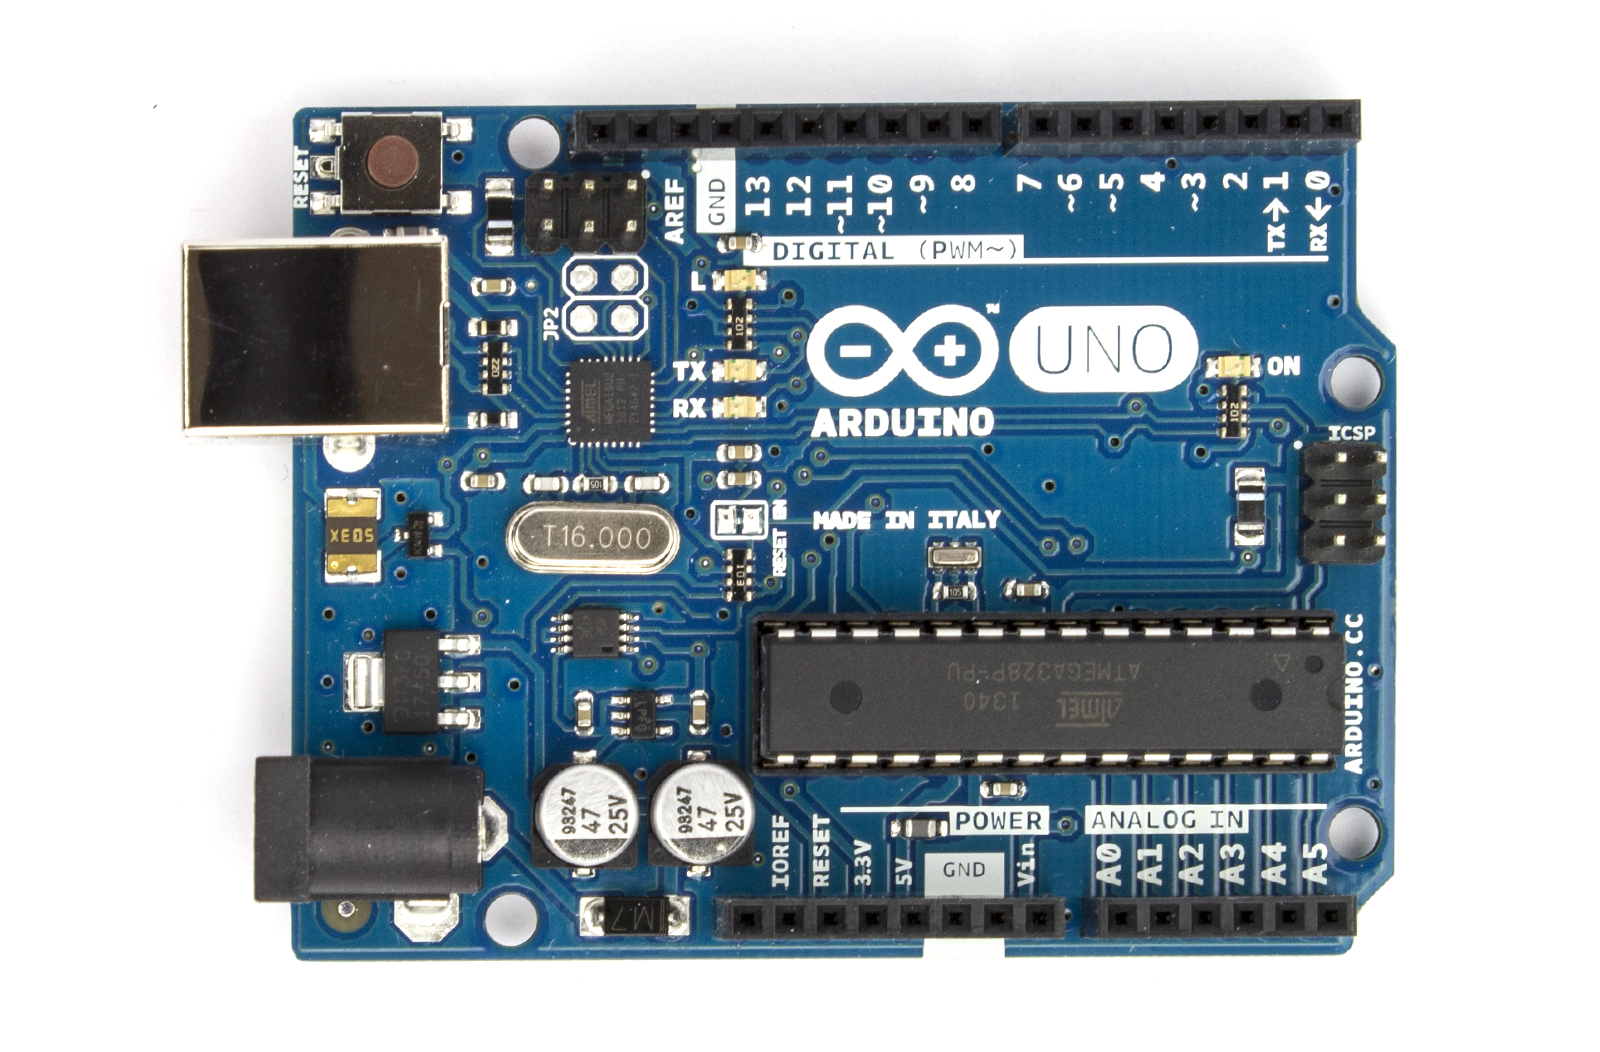
\includegraphics[scale=0.09]{Images/ArduinoUno}
\label{fig:arduinouno}
}\\
\subfloat[HC-06 Bluetooth Module for Arduino\textsuperscript{\cite{hc06ebay}}]{
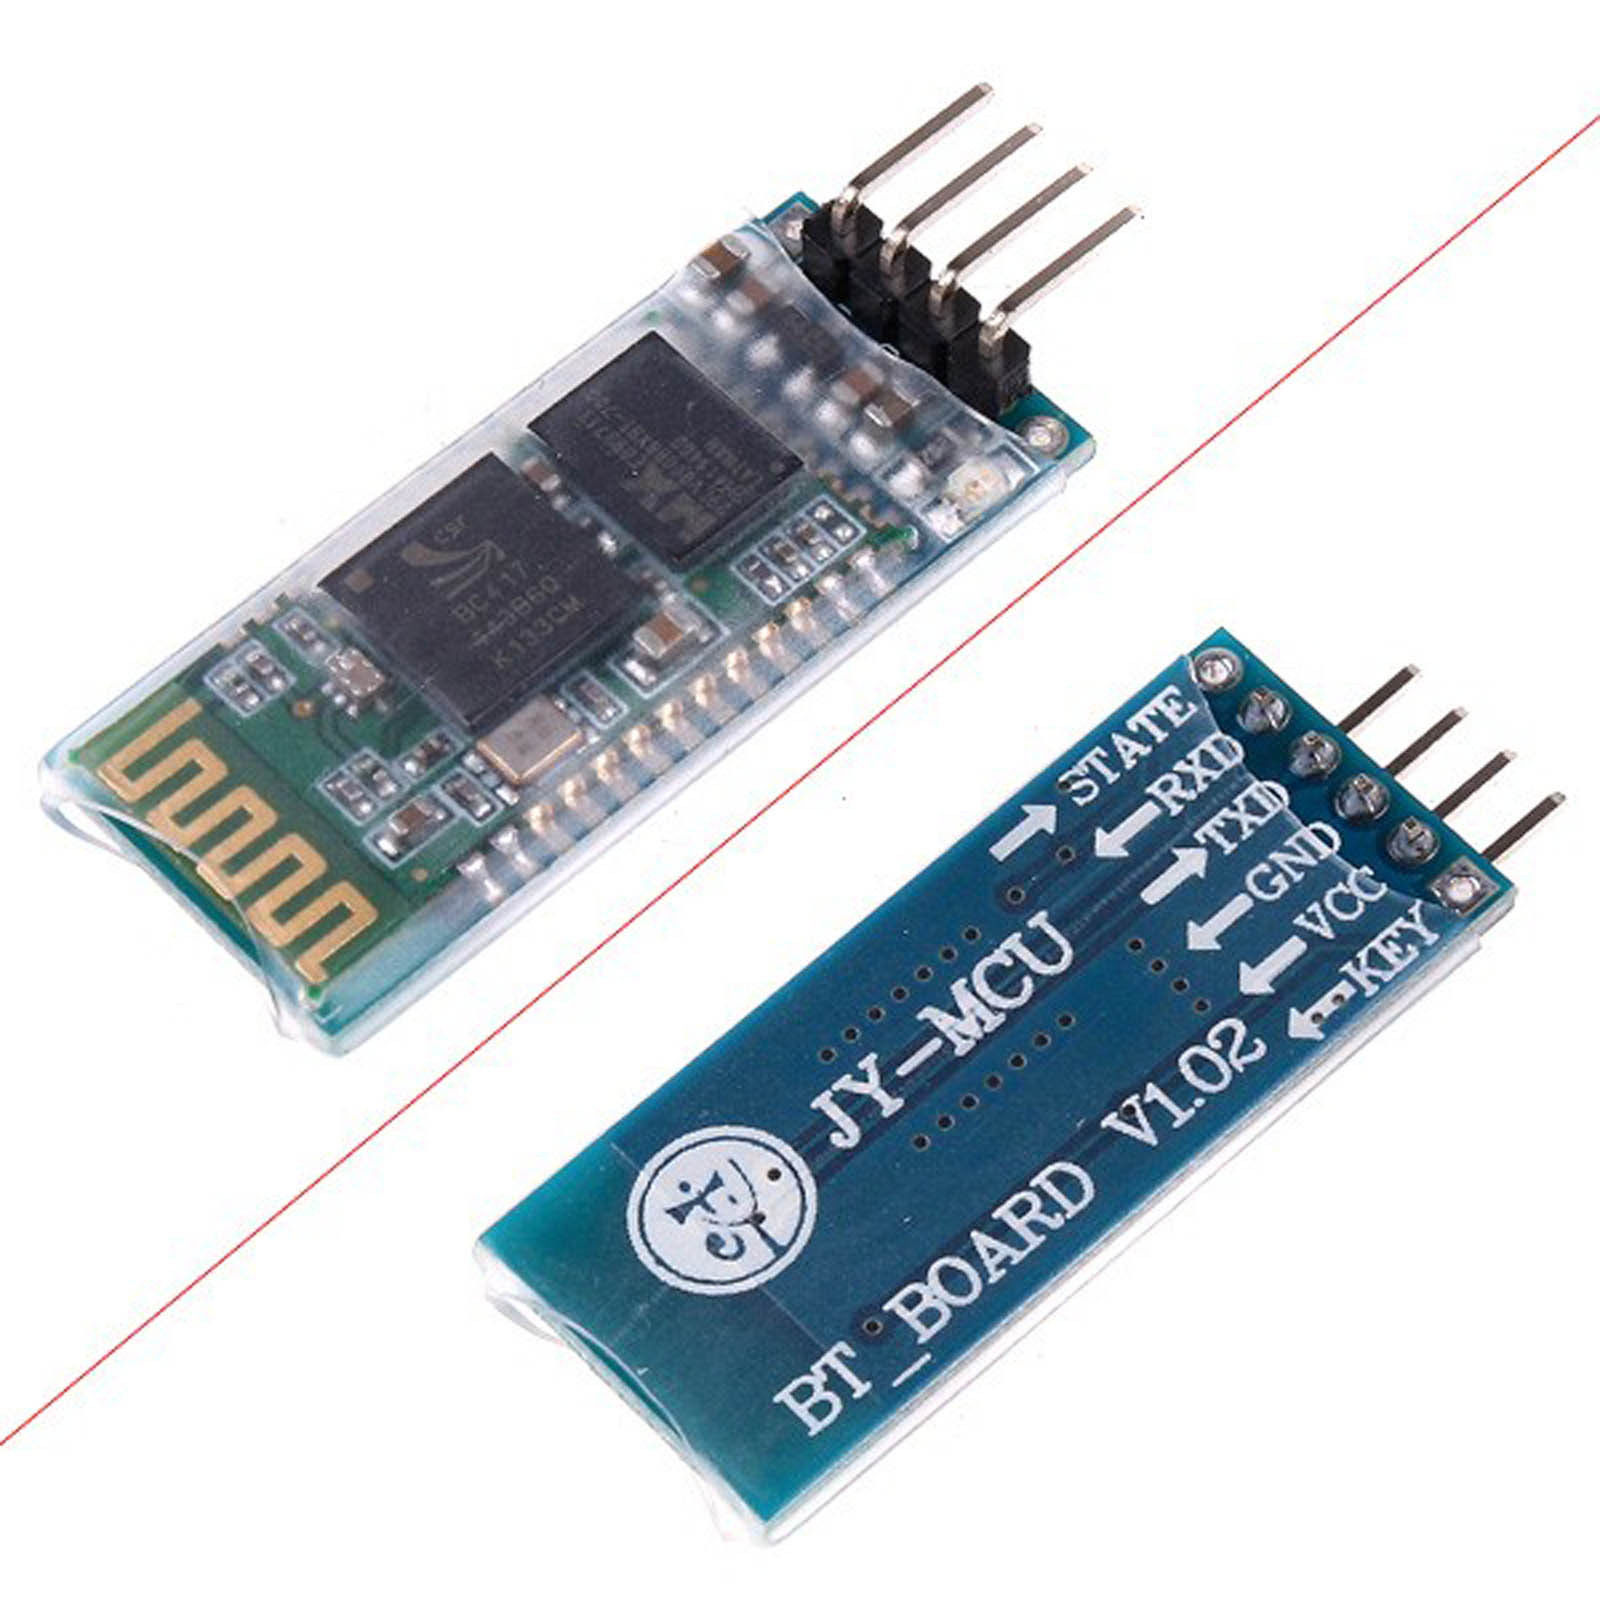
\includegraphics[scale=0.07]{Images/hc06pic}
\label{fig:hc06}
}
\caption{Arduino Development Kit used for Prototyping}
\label{fig:btarduino}
\end{wrapfigure}

\subsubsection{Data Transmission}

The purpose of the microcontroller in the PAWS Board design is to sample the audio signal from the microphone circuitry and transmit the data to the Interface. The data transmission could be done through a wired USB cable or wirelessly using Bluetooth, with both methods using standard serial transmission protocols. 

I tested the streaming of data wirelessly in real-time by connecting a HC-06 (JY-MCU) Bluetooth Module to an Arduino Uno, both of which are shown in Figure~\ref{fig:btarduino}. The Arduino Uno is a development board aimed at hobbyists built around an Atmel ATMEGA328P-PU microcontroller. The microcontroller can be programmed through Arduino's bespoke integrated development environment (IDE) that can be downloaded for free from Arduino's website\textsuperscript{\cite{arduinosite}} alongside documentation for the Uno board itself.
The HC-06 Bluetooth Module can easily be attached to the Serial outputs of the microcontroller through a simple circuit, shown in Appendix~\ref{arduinobluetooth}.

The ATMEGA microcontroller can be programmed through Arduino's IDE to read analogue signals with its built in analogue-to-digital-converter (ADC) and output the read data to the HC-06 Bluetooth Module through the microcontroller's serial ports. I used a smartphone-based bluetooth terminal app to connect with the HC-06 module to ensure that it transmitted all the data sent to it by the microcontroller correctly.

Certain elements of the Interface design were also tested using Matlab. I wrote Matlab scripts that would connect to the Arduino's serial bus (via USB) and read the incoming data from the Arduino Uno. I tested various methods to read in data, using infinite read and store loops for asynchronous input, and timed interrupts for a fixed data reception rate. I was not, however, able to connect to the Arduino through Bluetooth using Matlab, so after initially testing data transmission, I quickly moved on to developing an implementation plan for the Interface, with which Bluetooth transmission could be tested. 


\subsubsection{Programming the Software Interface}

The Interface has been designed as a computer application for the user to graphically control the functionality of a connected PAWS Board, or rather, its microcontroller component. The Interface is required to provide a graphical user interface (GUI) to allow the user to control the signal processing chain. The easiest way to implement this program was by using the \emph{Python} programming language. Python is an incredibly high-level language that is simple to write and can be used with a variety of signal processing and user-interface libraries. Libraries such as \emph{Pydub}\textsuperscript{\cite{pydub}} and \emph{PyAudio}\textsuperscript{\cite{pyaudio}} were found to integrate the ability to manipulate audio with the Python programming language but did not specifically meet the requirements of the Interface software, since they were designed more for handling audio files than real-time signals. The \emph{PyO}\textsuperscript{\cite{pyolibrary}} library is specifically designed for digital signal processing (DSP) in Python and allowed the Interface to be able to process audio signals in order to complete the user's tasks. The article \emph{Python For Audio Signal Processing}\textsuperscript{\cite{pyasparticle}}, Glover et al., demonstrates the use of other libraries for manipulating audio using Python, which was useful for attempting to find the best solution for programming the Interface. 

\subsubsection{Sample File Triggering Simulation}

As an aid to crafting the Implementation Plan, I simulated how the 'Sample' function would work using a microphone signal to trigger preset files. Figure~\ref{fig:samptrigmatlab} shows the various processing stages of a simulation of triggering a sound file of a drum sample from recorded audio. 

The raw recording was of a rhythm being tapped into the microphone of my smartphone. The recording then underwent very basic filtering and transient detection processes to produce pulses that were used to finally trigger the chosen drum sample. As we can see, the microphone taps were recognised correctly as triggers by the system and therefore produced a drum beat\footnotemark[1] of the same rhythm, although slightly latent than the original recording. In this instance, the raw recording was not contaminated with much noise, which may not be the case with the PAWS Board, and was also processed offline whereas the PAWS Board's audio stream will be processed in real-time and thus will be prone to more computational complications. 

\footnotetext[1]{A note of interest: the Drum Output plot shows the two stereo channels of the drum sample overlaid atop one another (one in orange, the other in blue), and this visual served to inspire how I went about implementing a waveform display in my later prototypes.}

\begin{figure}[H]
\centering
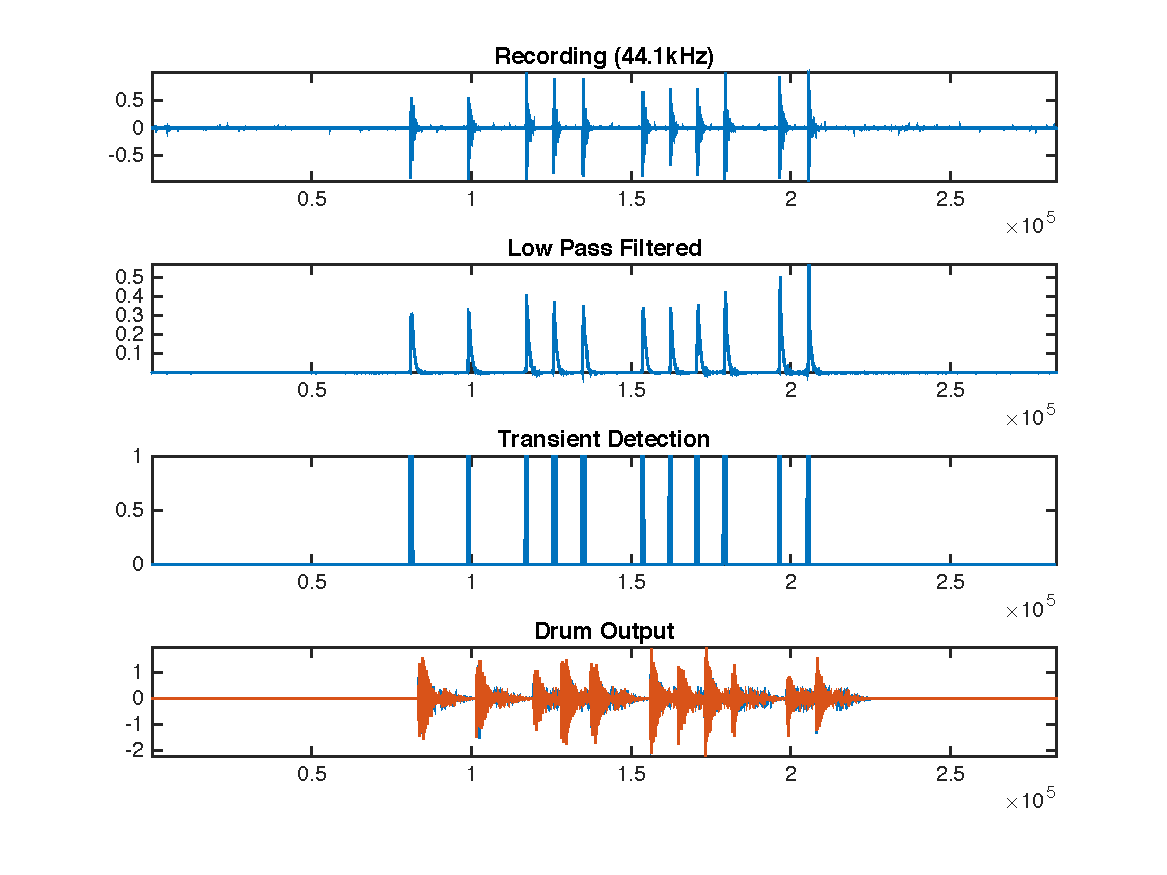
\includegraphics[width = 0.6\textheight, height = 0.45\textheight]{Images/slaptodrum.pdf}
\caption{Simulation of Sample Triggering algorithm in Matlab}
\label{fig:samptrigmatlab}
\end{figure}

\newpage
\section{Implementation Plan} \label{Implementation Plan}

After testing the various technologies I would require to implement each component of the System Design as described in Section~\ref{Implementation Design}, I produced a plan to guide and direct the Implementation process. The instrument was broken down into successive stages of prototyping, with each prototype implementing a key feature of the System Design. Table~\ref{tab:listofprototypes} details the planned development of prototypes and their key features, with each subsequent prototype building upon the previous in terms of functionality or user experience. Each version of Prototype 0.1.xx was given a week to be tested and implemented, and the rest were given a fortnight, although this would of course change depending on further analyses of what their implementations would require in terms of research and resources. 

Prototype 0.1.xx was designed to be a fully functioning program with digital gain control, wireless transmission and a separate power source for the PAWS Board. The Interface was to be programmed using Python, the microphone circuit was initially built on Breadboard for easy testing, and the Arduino was used to transfer data between the two. Each part of Prototype 0.1.xx looked at implementing a particular functionality to gradually build up a fully featured PAWS Board and counterpart Interface. All following prototypes focussed on further developments such as a Quantisation function to quantise any incoming 'taps' to a discrete time grid, or a Harmonisation function to trigger background harmonies depending on the primary audio generated by the user, as briefly described in Section~\ref{Product Concept} Product Concept. 


\begin{table}[H]
\begin{center}
\begin{tabular}{|l l}
Prototype  &   Features \\ \hline \hline
0.1.01 &    Basic output of microphone and simple Sample Triggering function \\
0.1.02 &    Cleaner microphone signal, single GUI\footnotemark[1] for Interface with both Voice and Sample functions     \\
0.1.03 &  PGA\footnotemark[2] in circuit for digital gain control   \\
0.1.04 &  Bluetooth transmission  \\
0.1.05 &  A fully featured GUI for user control   \\ \hline
0.2.xx &  All hardware on PCBs\footnotemark[3] and 3D printed wearable housings    \\
0.3.xx &  Integration of SP\footnotemark[4] functions such as Gain, EQ\footnotemark[5], Pitch Detection \& Correction     \\
0.4.xx &  Quantisation Function\footnotemark[6]    \\
0.5.xx &  Harmonisation Function\footnotemark[7]    \\
0.6.xx &  Integrate Accelerometer onto PAWS Board and develop Motion feature on Interface    \\
\end{tabular}
\end{center}
\caption{Implementation Plan as a List of Prototypes and their Features}
\label{tab:listofprototypes}
\end{table}

\footnotetext[1]{GUI: Graphical User Interface}
\footnotetext[2]{PGA: Programmable Gain Amplifier}
\footnotetext[3]{PCB: Printed Circuit Board}
\footnotetext[4]{SP: Signal Processing}
\footnotetext[5]{EQ: Equalisation}
\footnotetext[6]{Quantisation Function: User can tap a tempo to quantise all produced sample sounds} 
\footnotetext[7]{Harmonisation Function: User can trigger virtual instrument samples to harmonise with their singing} 


\begin{wraptable}[16]{r}{0.3\textheight}
\begin{center}
\begin{tabular}{|l r}
Prototype   &   Projected Completion \\
& Date (2015)\\ \hline
0.1.01  &   20 Jan \\ \hline
\hline \emph{Interim Report} & 2 Feb \\ \hline \hline
0.1.02  & 11 Feb\\ 
0.1.03  & 17 Feb\\ 
0.1.04  & 20 Feb\\ 
0.1.05  & 28 Feb\\ \hline
0.2.xx  & 18 Mar\\
0.3.xx  & 1 Apr\\
0.4.xx  & 17 Apr\\
0.5.xx  & 1 May\\
0.6.xx  & 15 May\\ \hline
\hline \emph{Abstract} & 8 Jun \\ \hline
\hline \emph{Final Report} & 17 Jun \\ \hline
\hline \emph{Presentation} & 24 Jun \\ \hline
\end{tabular}
\end{center}
\caption{Implementation Plan as a Timetable of Deliverables}
\label{tab:implementationplan}
\end{wraptable}



Table~\ref{tab:implementationplan} shows the estimated completion dates for each Prototype, alongside the submission dates for all project deliverables.

Prototype 0.1.01 was completed before the Interim Report and Prototype 0.1.05 was estimated to be functioning by the end of February 2015. This prototype was designed to meet all of the basic specifications of the PAWS instrument designed for implementation. The months of March to May were dedicated to improvements and enhancements upon either the functionality, what the user could do with the instrument, or usability, how the user could interact with the instrument. This production plan ensured that, no matter the progress, there would always be a version of the musical instrument that was functional across all of its basic requirements.


\newpage
%%%%%%%%%%%%%%%%%%%%%%%%%%%%%%%%%%%%%%%%%%%%%
\section{Product Implementation} \label{Implementation}

This section describes the implementation of a PAWS Board, starting with an Arduino Uno and a microphone circuit on breadboard and ending with three microphone circuits on Printed Circuit Boards worn on a user's fingers with 3D printed Rings, and that of a software Interface application that underwent a vast evolution in terms of functionality and interactivity. This section summarises the steps taken to get from the starting stage to the final prototype and provides details on the key features of each developed prototype and how they build upon their predecessors. 

\subsection{Prototype 0.1.01} \label{0101}

\begin{wrapfigure}{r}{0.35\textheight}
\centering
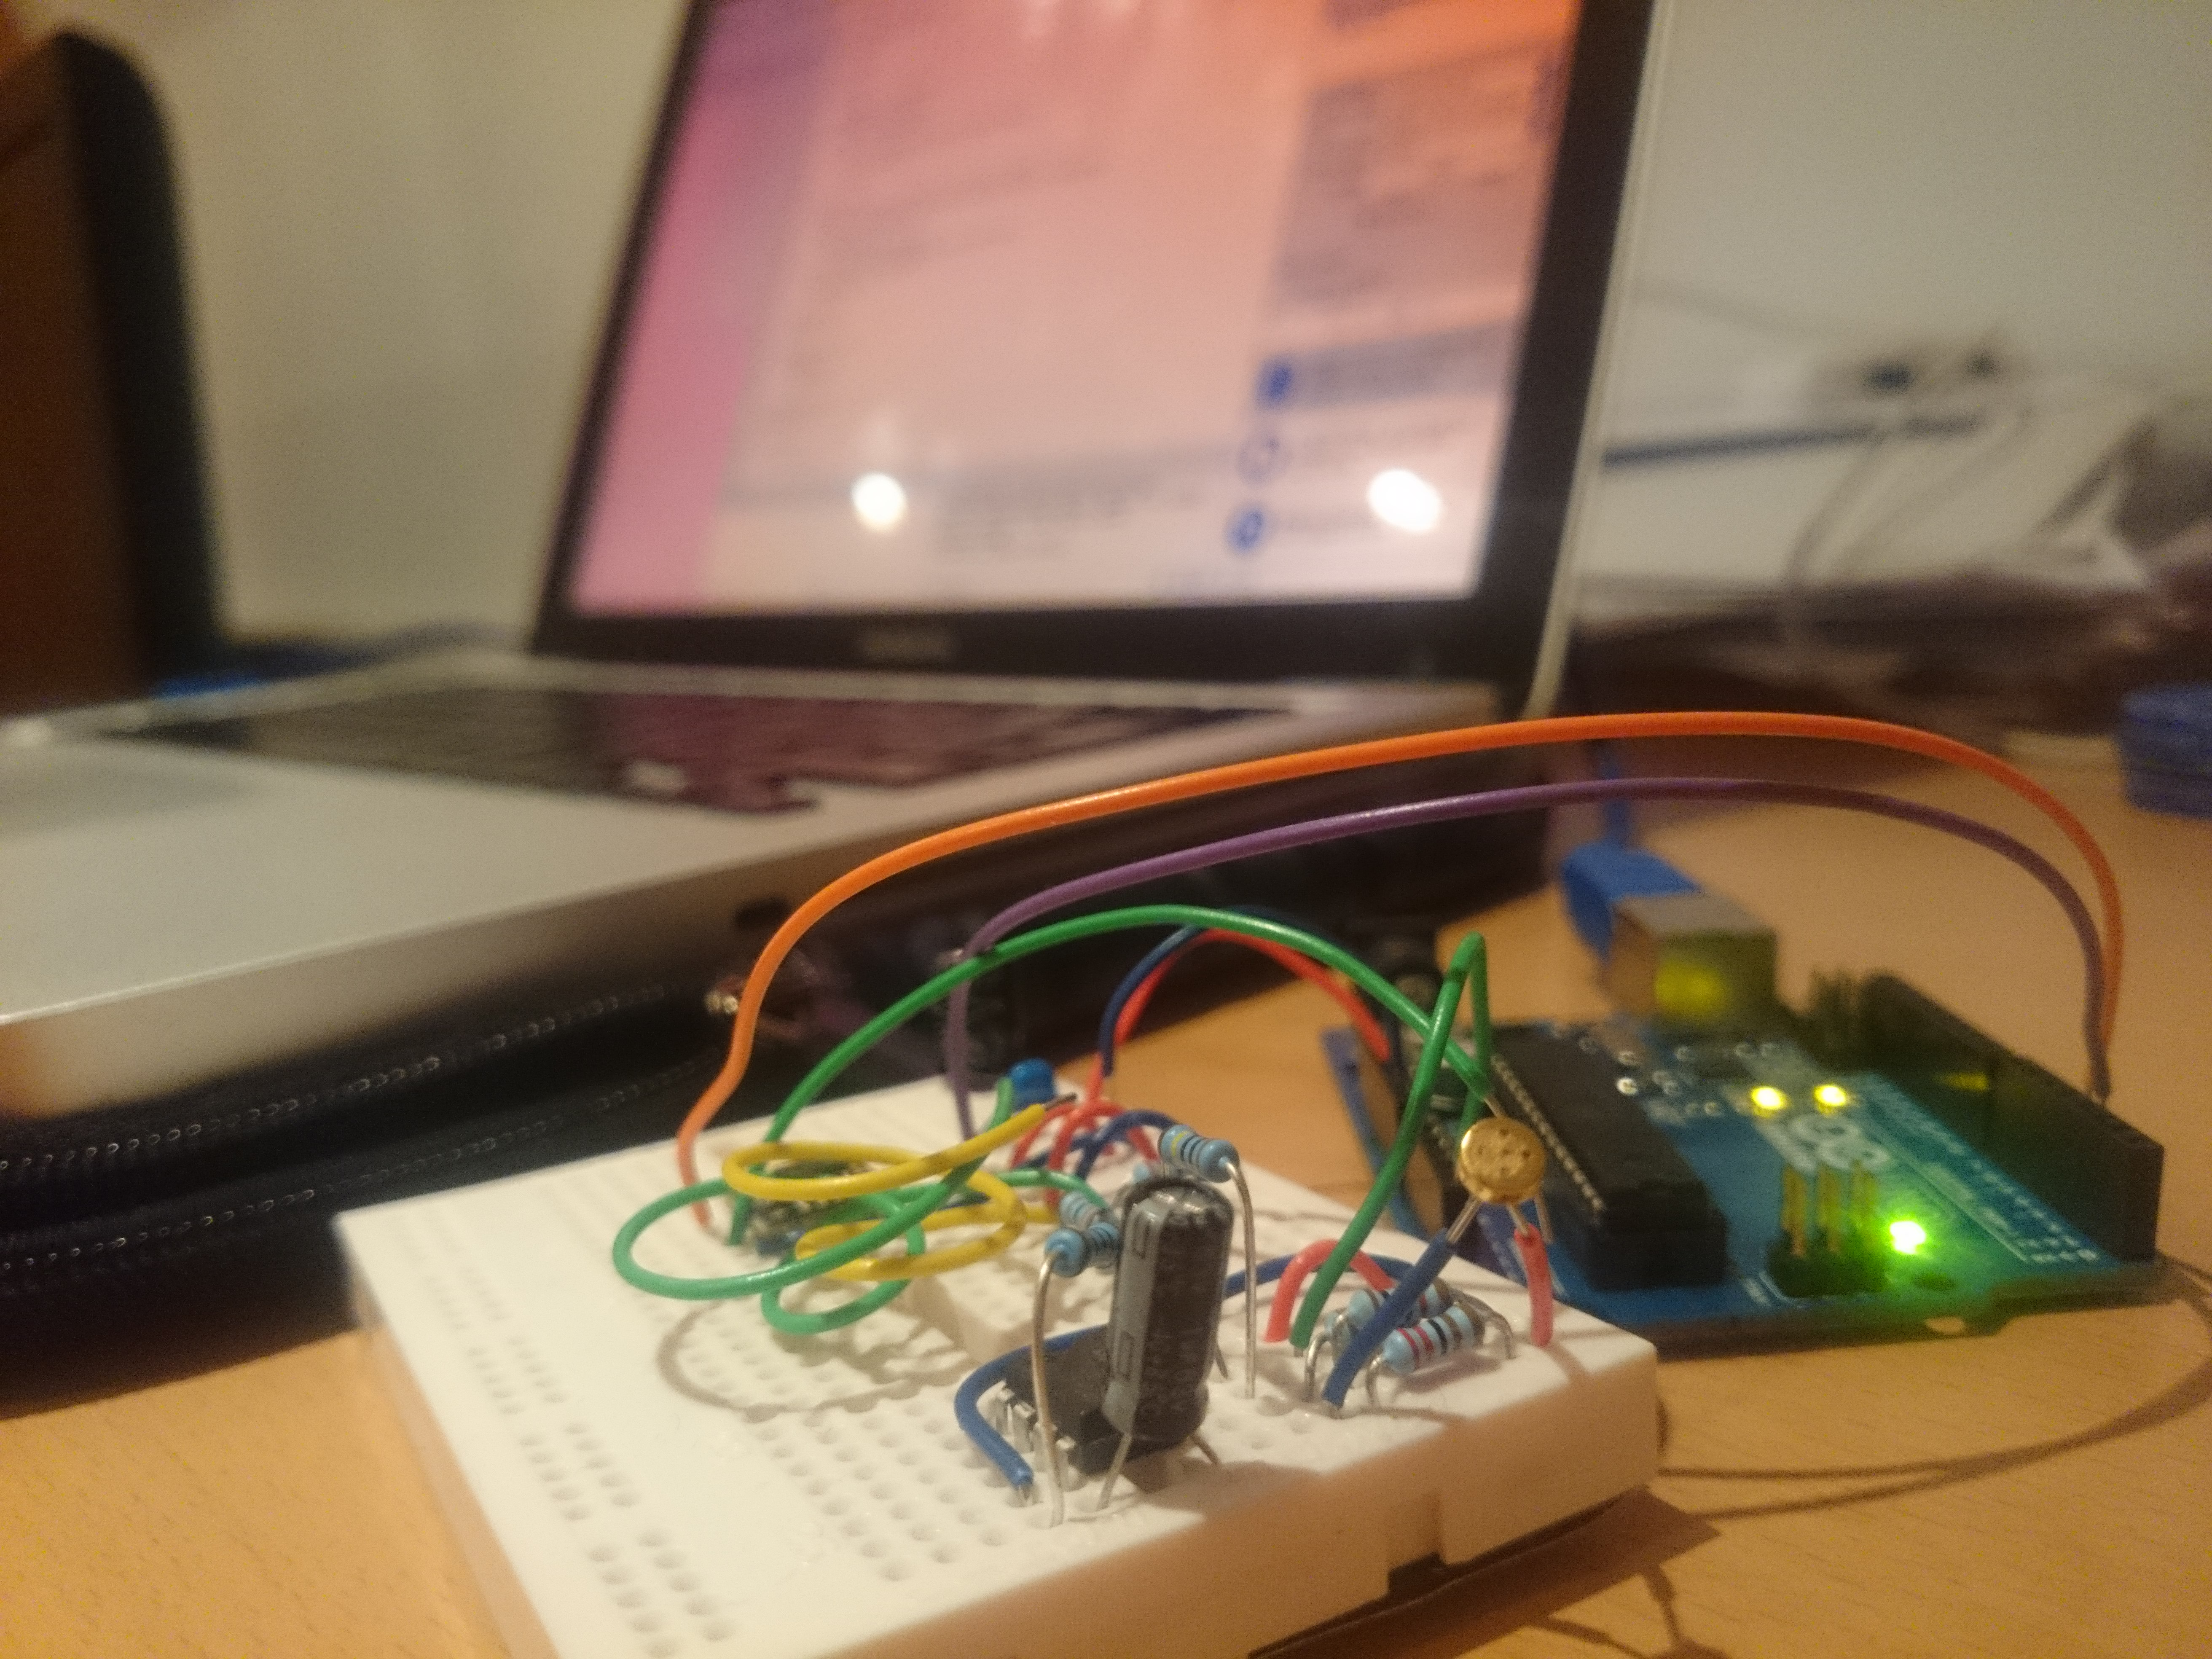
\includegraphics[scale = 0.045]{Images/prototype101board}
\caption{Photograph of setup, Prototype 0.1.01}
\label{fig:101board}
\end{wrapfigure}


Prototype 0.1.01 was the very first realisation of the PAWS instrument. Figure~\ref{fig:101board} shows the microphone circuit implemented on Breadboard and connected to the Arduino Uno development board. The Breadboard included connections for a Bluetooth module and a Programmable Gain Amplifier (PGA) wired for testing but these were not utilised for this current prototype. The circuit comprised of a microphone connected to the Atmel ATMEGA328 microcontroller through a gain stage. The microcontroller was programmed to stream the audio data to the Serial bus, which was connected to the Interface on my laptop via a USB cable. The Interface was programmed in Python to read data from the Serial bus and output it to the laptop's audio device, which I could hear through speakers or headphones. A library called \emph{PyO}\textsuperscript{\cite{pyolibrary}}, written for implementing digital signal processing (DSP) functions, was used to generate two Python scripts: one to play whatever audio the microphone captured, the 'Voice' function, and another to trigger drum samples in response to the microphone being tapped with a finger, the 'Sample' function.

This prototype was able to play the audio captured by the microphone, although it was fairly distorted due to digital noise from the Arduino feeding into the signal path. The prototype was also able to trigger drum sounds as the microphone was slapped. However, the interface was not yet programmed to filter the raw input and detect the transients in a clean manner and therefore the produced drum sounds had a slight latency and sometimes misfired, i.e. they played when not supposed to.

\begin{wrapfigure}[13]{r}{0.4\textheight}
\centering
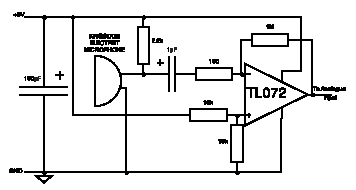
\includegraphics[scale=1.5]{Images/mic0101}
\caption{Microphone Circuit with Op Amp Gain Stage, Prototype 0.1.01}
\label{fig:101circuit}
\end{wrapfigure}

\subsubsection{Microphone Circuit}

Figure~\ref{fig:101circuit} shows the microphone circuit designed for this Prototype. The microphone, connected as described in its datasheet\textsuperscript{\cite{kingstatedatasheet}}, was fed into a TL072 Operational Amplifier with a gain of ten thousand to boost the audio signal to within the dynamic range of the microcontroller's Analogue-to-Digital Converter (ADC). This prototype used the 5V power rails provided by the Arduino and was therefore laced with digital noise. Thus, a 100{$\mu$}F electrolytic capacitor was placed across the rails in an attempt to reduce this noise.  

\newpage
\subsubsection{Microcontroller Program}

The microcontroller program used a timed interrupt to read a value from its input analogue pin at a set frequency of 8kHz and this value was added to a global circular buffer. In the main program loop, the values in this circular buffer were printed to the Serial bus. The printing of sample values to the Serial bus could not be handled inside the interrupt function as it took much longer to process than the frequency of the function call. Therefore, the print to Serial process was handled in the main program loop, which lead to potential inaccuracies due to the two functions writing to and reading from the circular buffer at different frequencies. A dynamically allocated queue was tried and tested with the Arduino libraries \emph{QueueList}\textsuperscript{\cite{queuelist}} and \emph{QueueArray}\textsuperscript{\cite{queuearray}}, but they seemed to be unable to cope with the speed at which the data was being read. Appendix~\ref{mcflow} shows a flowchart diagram of how the microcontroller was programmed.

\subsubsection{Interface - 'Voice' Mode}

Programming the Python Interface to read from the Serial bus was well-documented in the \emph{pySerial}\textsuperscript{\cite{pyserial}} library and was therefore very straightforward to implement. Each read sample was appended to a Python list variable, used like a buffer queue, as a \emph{PyO} signal, ready for processing.

The first version of the Interface was developed to simply take the input signal buffer and output it to the core audio device, and thereafter clear the samples that had been played from the buffer. The \emph{PyO} library used an audio server to receive data samples asynchronously and output them at the user-defined sampling rate. Therefore, it was simple enough to program an infinite loop to constantly read in samples from the Serial bus and write them to the output server. Appendix~\ref{interfaceflow} shows a flowchart describing the processes involved in this Interface program. 

\subsubsection{Interface - 'Sample' Mode}

Another version of the Interface was created where data samples were read in chunks from the Serial bus, compared against an intuitively-set threshold value and the generated on/off pulses were used to send the waveform of a drum sound to the output audio server. This method was done in the most basic manner in order to quickly demonstrate that it could indeed be done. The Prototype was able to play drum sounds when the microphone was struck but there seemed to be a small delay between the two events. There were also many misfires, or drum sounds being played when they were not supposed to, due to the roughly implemented spike detection method. Appendix~\ref{interfaceflow} shows how this particular Prototype implemented the sample triggering function.

\subsection{Prototype 0.1.02} \label{0102}

\begin{wrapfigure}[12]{r}{0.4\textheight}
\centering
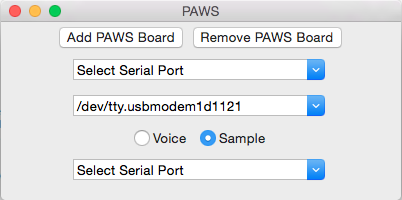
\includegraphics[scale=0.6]{Images/pyblue_play}
\caption{User Controls developed for the Interface, Prototype 0.1.02}
\label{fig:pyblue_play}
\end{wrapfigure}

Prototype 0.1.02 involved the creation of a Graphical User Interface (GUI) to control the 'Voice' and 'Sample' modes previously coded through a single control panel. 

\subsubsection{Building a GUI}

The GUI was built using a library called \textit{wxPython}\textsuperscript{\cite{wxpython}}, and as seen in Figure~\ref{fig:pyblue_play} featured top level buttons to 'Add' and 'Remove' boards. Each addition of a PAWS Board generated a drop-down list of serial ports to connect to, and once connected to the Arduino, radio buttons for programming the Board in a particular mode were shown. 

The back end of the program required to work with the GUI was trickier to implement. Appendix~\ref{pyblue_flow} shows a flow chart to demonstrate the workings of the code. Upon startup, the audio server and GUI were set up. The 'Add PAWS Board' button created a virtual \textit{Bus} to store information on the selected serial port and function flags to determine whether the program should be in 'Voice' mode or 'Sample' mode. When a serial port was chosen from the drop-down list on the GUI, a function was called to open the port and ready it for data transfer. The function-selection radio buttons called the respective 'Voice' or 'Sample' functions in a new high-level thread to simultaneously process the incoming audio data while continuously listening for events on the GUI. The 'Voice' and 'Sample' functions ran endlessly based on their respective flags. Only one flag was allowed to be active at any time and the dropping of a flag caused the respective function to exit. The 'Remove PAWS Board' was programmed to reset the data stored in the last created virtual Bus, closing all serial connections and running threads in the process, and would then remove all control elements for that Board from the GUI. Upon quitting the Interface, all Busses were disconnected and closed and all flags were dropped to allow all running threads to finish correctly. 

The GUI itself used Sizers, a \textit{wxPython} functionality, that allowed for elements to be dynamically grouped together. This meant that I was able to simply display the 'Add PAWS Board' button upon startup, which when pressed would make the 'Remove' button visible and then would create a 'Select Serial Port' drop down list on the GUI and a corresponding virtual Bus in the back end. A function to read all available serial ports was also called to populate the drop down lists on the GUI. Adding more Boards would result in the creation of more virtual Busses and Serial Port lists for the user to interact with. If a valid Serial Port was selected, the radio buttons for selecting the required mode would then be displayed. 


\subsection{Prototype 0.1.03} \label{0103}

This prototype made significant changes to the microphone circuit. A Programmable Gain Amplifier (PGA) was bought and tested against the previously implemented TL072 Operational Amplifier. The Arduino's functionality was also optimised to remove some of the redundancies found in Prototype 0.1.01.

\subsubsection{Improving the Operational Amplifier Circuit}

\begin{wrapfigure}[15]{r}{0.4\textheight}
\centering
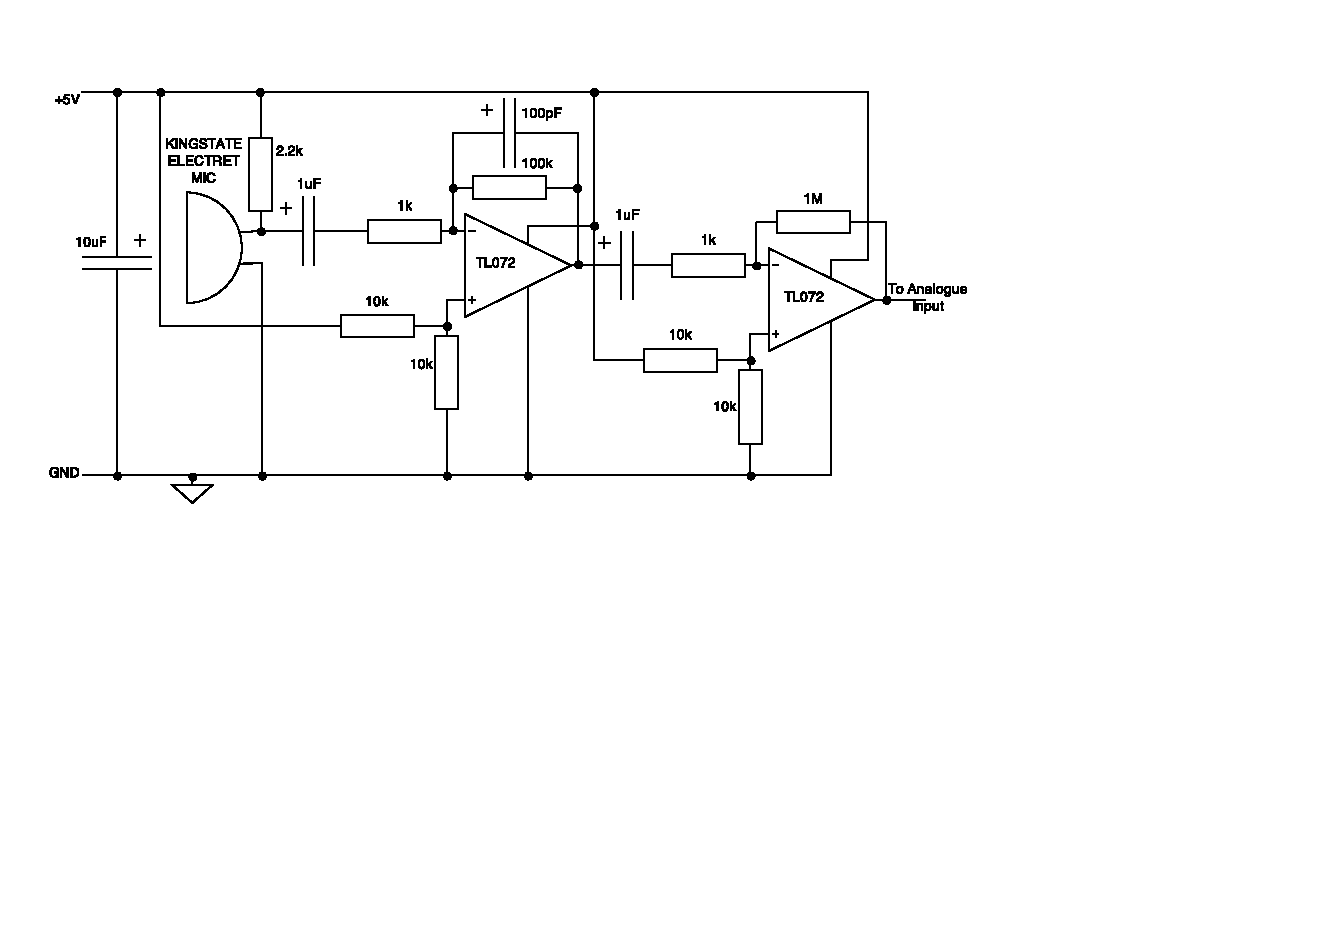
\includegraphics[scale=0.6]{Images/TL072circuit_2}
\caption{Microphone Circuit with Improved Op Amp Gain Stage, Prototype 0.1.03}
\label{fig:103opamp}
\end{wrapfigure}

The Operational Amplifier designed in Prototype 0.1.01 (Figure~\ref{fig:101circuit}) was improved for better performance. One of the key problems of the initial circuit was that a single amplifier was being used to provide a gain of 10,000 or 80dB. Since I was using a dual-TL072 chip, it made sense to use two-stages for amplification, with an overall gain of 80dB but with each stage only providing a fraction of that. This would release the strain on each amplifier and meant that my signal would no longer be inverted at the input to the Arduino's ADC. 

In the first design, the 1$\mu$F decoupling capacitor and the gain resistor at the input of the op amp was generating a high pass pole at 1.5kHz, which was significantly damaging the audio signal but leaving much of the high frequency thermal noise alone. To fix this, the input resistor of each op amp was set to 1k$\Omega$ to create a second order high pass filter at 159Hz such that it did not impact as much upon the audio signal. A first order low pass filter was created using the feedback loop of the first amplifier stage to remove frequencies above 15.9kHz, which I found to ultimately correspond to thermal noise. 

After filtering the signal, I found that the overall gain was quite low so I set the feedback resistor of the second amplifier stage to 1M$\Omega$ to produce an overall gain of 100,000 or 100dB. 
The capacitor across the power rails was also reduced to 10$\mu$F as the previous 100$\mu$F one seemed unnecessarily large. Figure~\ref{fig:103opamp} shows the improved Op Amp circuit.  


\subsubsection{Implementing a Programmable Gain Amplifier}

I wished to implement a Programmable Gain Amplifier (PGA), which could be digital controlled to set the gain of the microphone circuit. This would allow for future developments with automatic gain control algorithms should I wish to implement them. The PGA that I decided to buy was the \textit{AD605} by Analog Devices because its gain could be set with a simple analogue voltage and it was available as a Dual-Inline Package, useful for testing on breadboard, as well as in surface mount for final implementation on a Printed Circuit Board. 

The AD605 was a two-stage amplifier whose gain value depended on a dedicated control signal. I was also able to set the amplification range by modifying two feedback resistors. Setting both resistors to 0$\Omega$ (i.e. short circuit) would give me a range of -28dB to 68.8dB and setting them to infinite (i.e. open circuit) would correspond to a range of 0dB to 96dB. Of course I opted for the latter as that was more appropriate for my circuit since I did not need to attenuate the microphone signal. I used a DC level capacitor to offset the input signal by 2.5V to ensure that its zero-level fell exactly in the centre of the input range for the Arduino's ADC. 
When designing the AD605 circuit, the input pins required decoupling capacitors which also set a high pass corner on the signal in conjunction with the pins' internal resistances. The internal resistance of each of the input pins was determined to be 175$\Omega$, and therefore decoupling capacitors no smaller than 9.09$\mu$F were required to ensure a high pass cutoff lower than 100Hz. I decided to set the values of these decoupling capacitors to 10$\mu$F to ensure that most of the audible range of frequencies (20Hz to 20kHz) was preserved. The output of the amplifier was also low pass filtered with a combination of an 82k$\Omega$ series resistor and a 100pF capacitor to ground connected to the Arduino's ADC input in order to remove all instances of thermal noise above a cutoff of 19.4kHz.  

\begin{wrapfigure}{r}{0.3\textheight}
%\begin{figure}[H]
\centering
\subfloat[AD605 Circuit]{
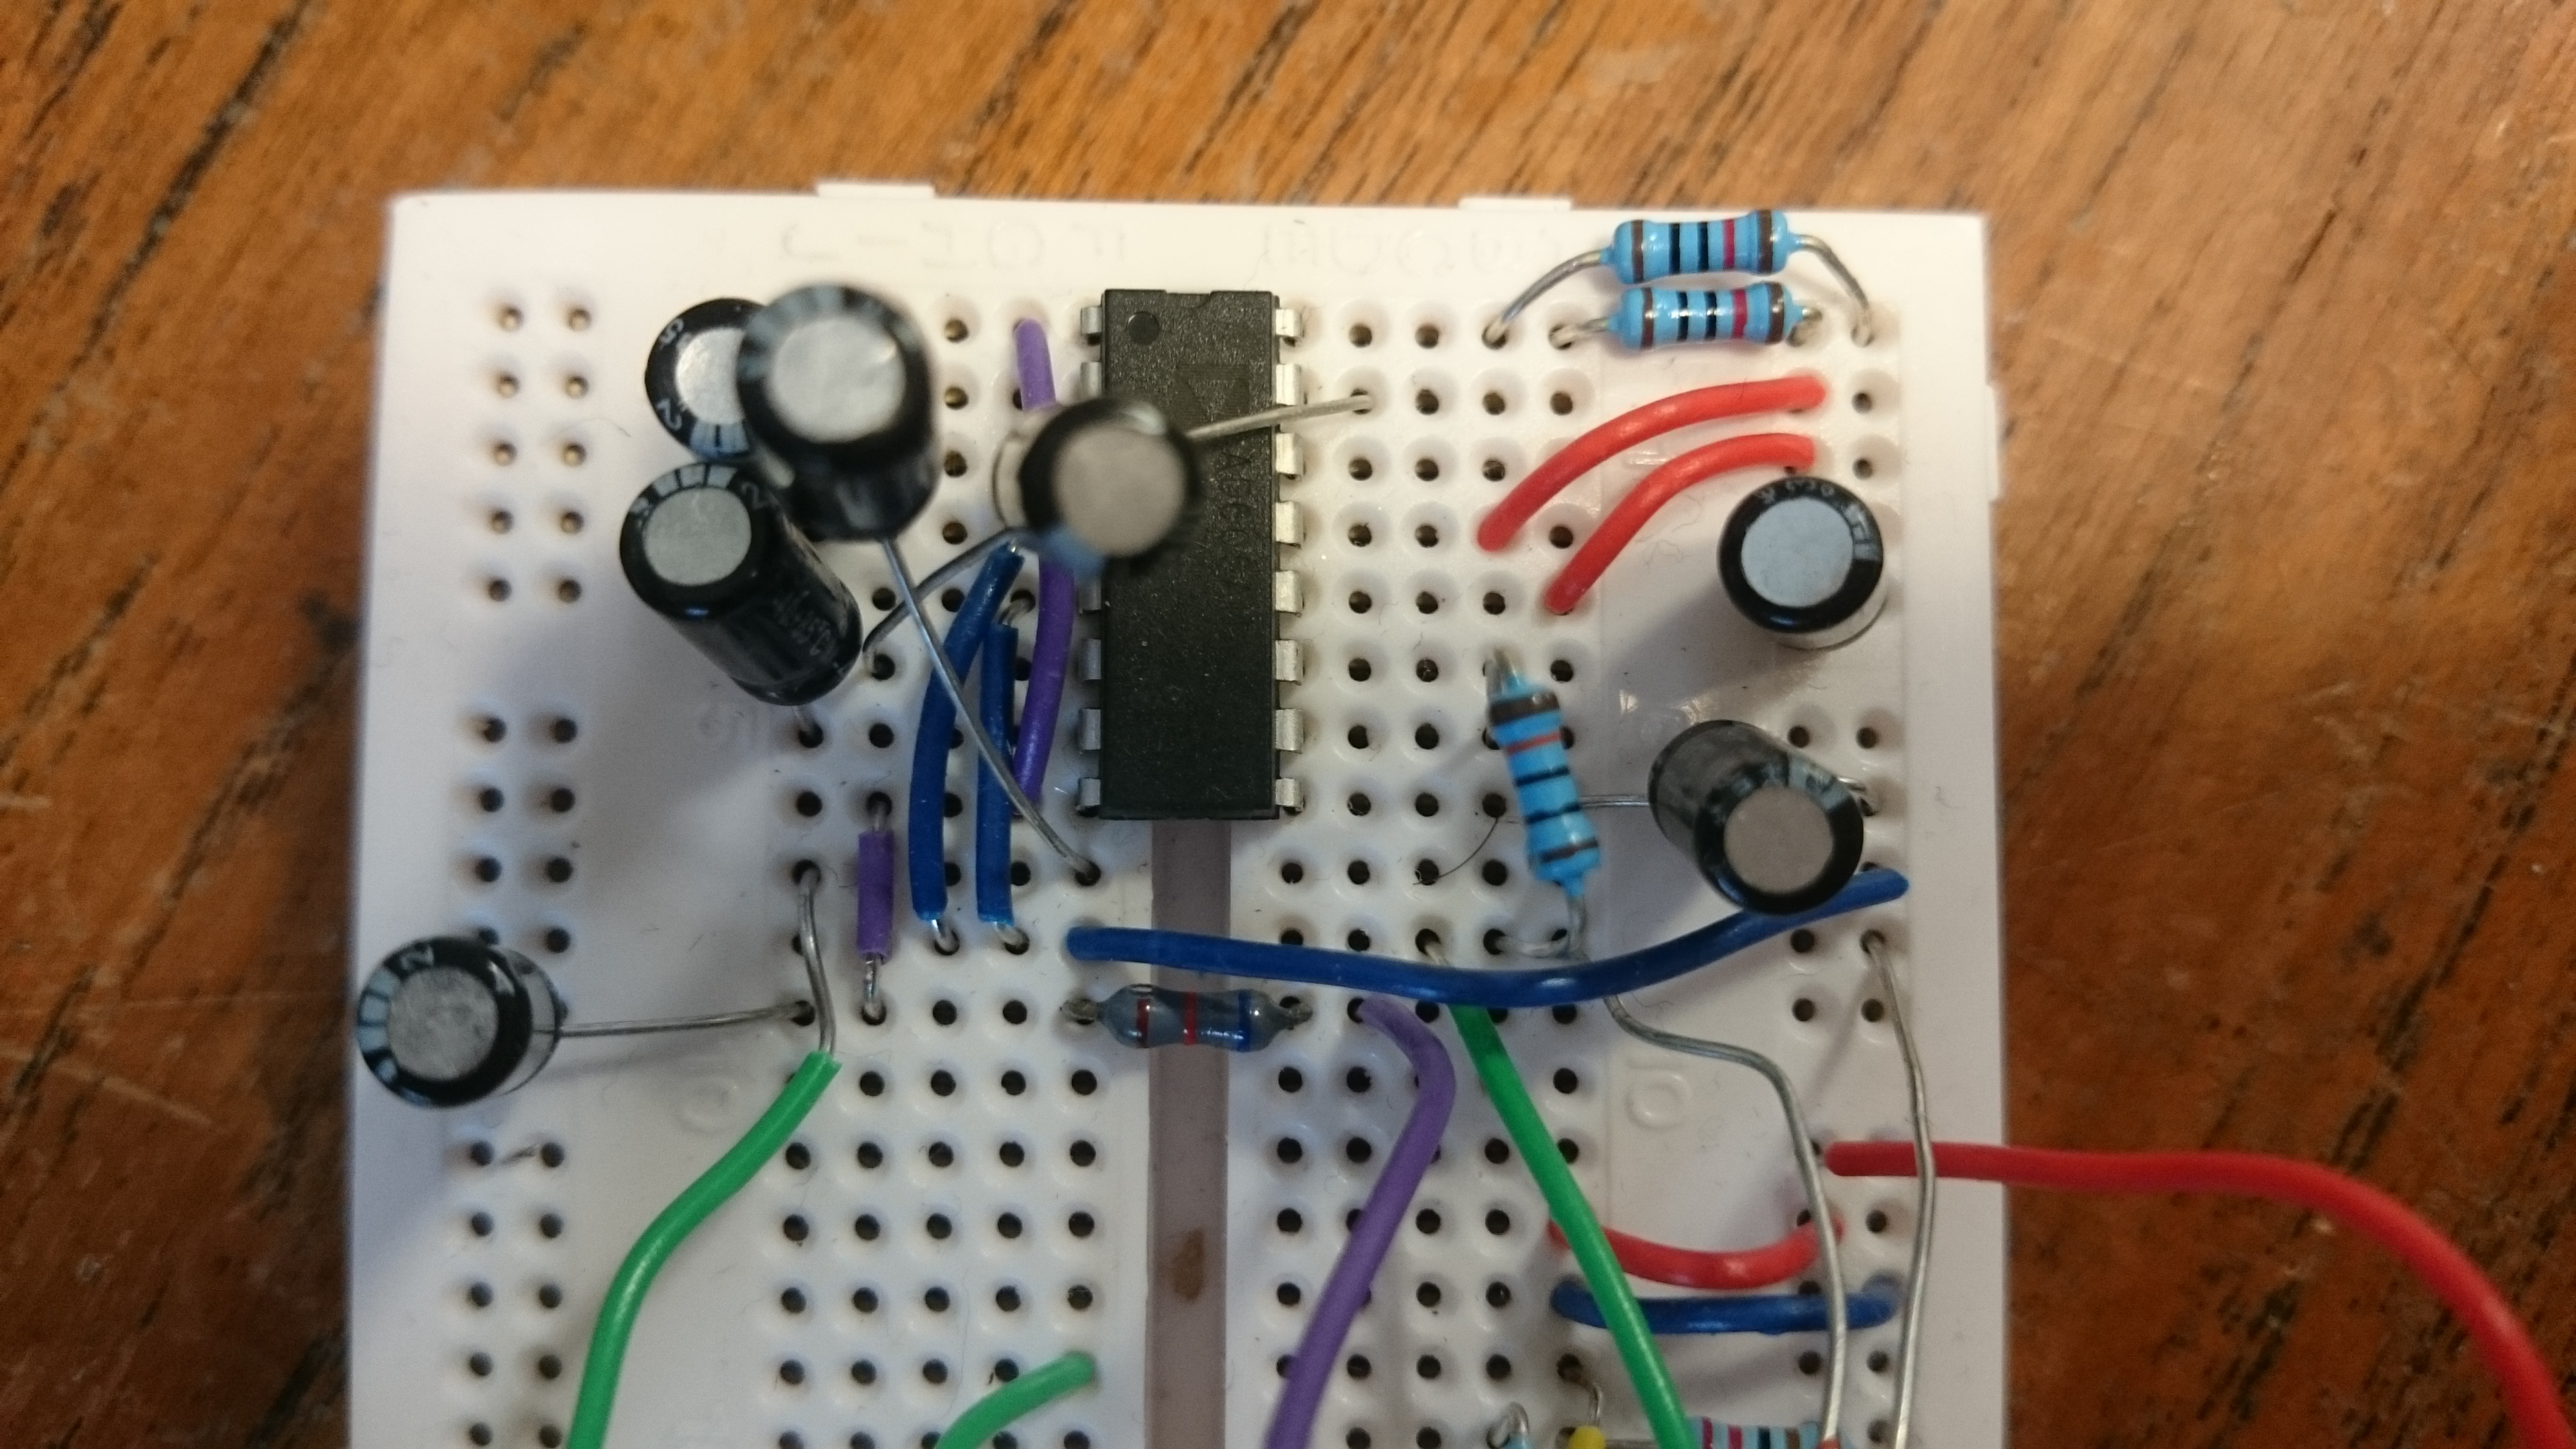
\includegraphics[scale = 0.05]{Images/ad605_circuit}
}\\
\subfloat[AD605 Circuit and Microphone on Veroboard]{
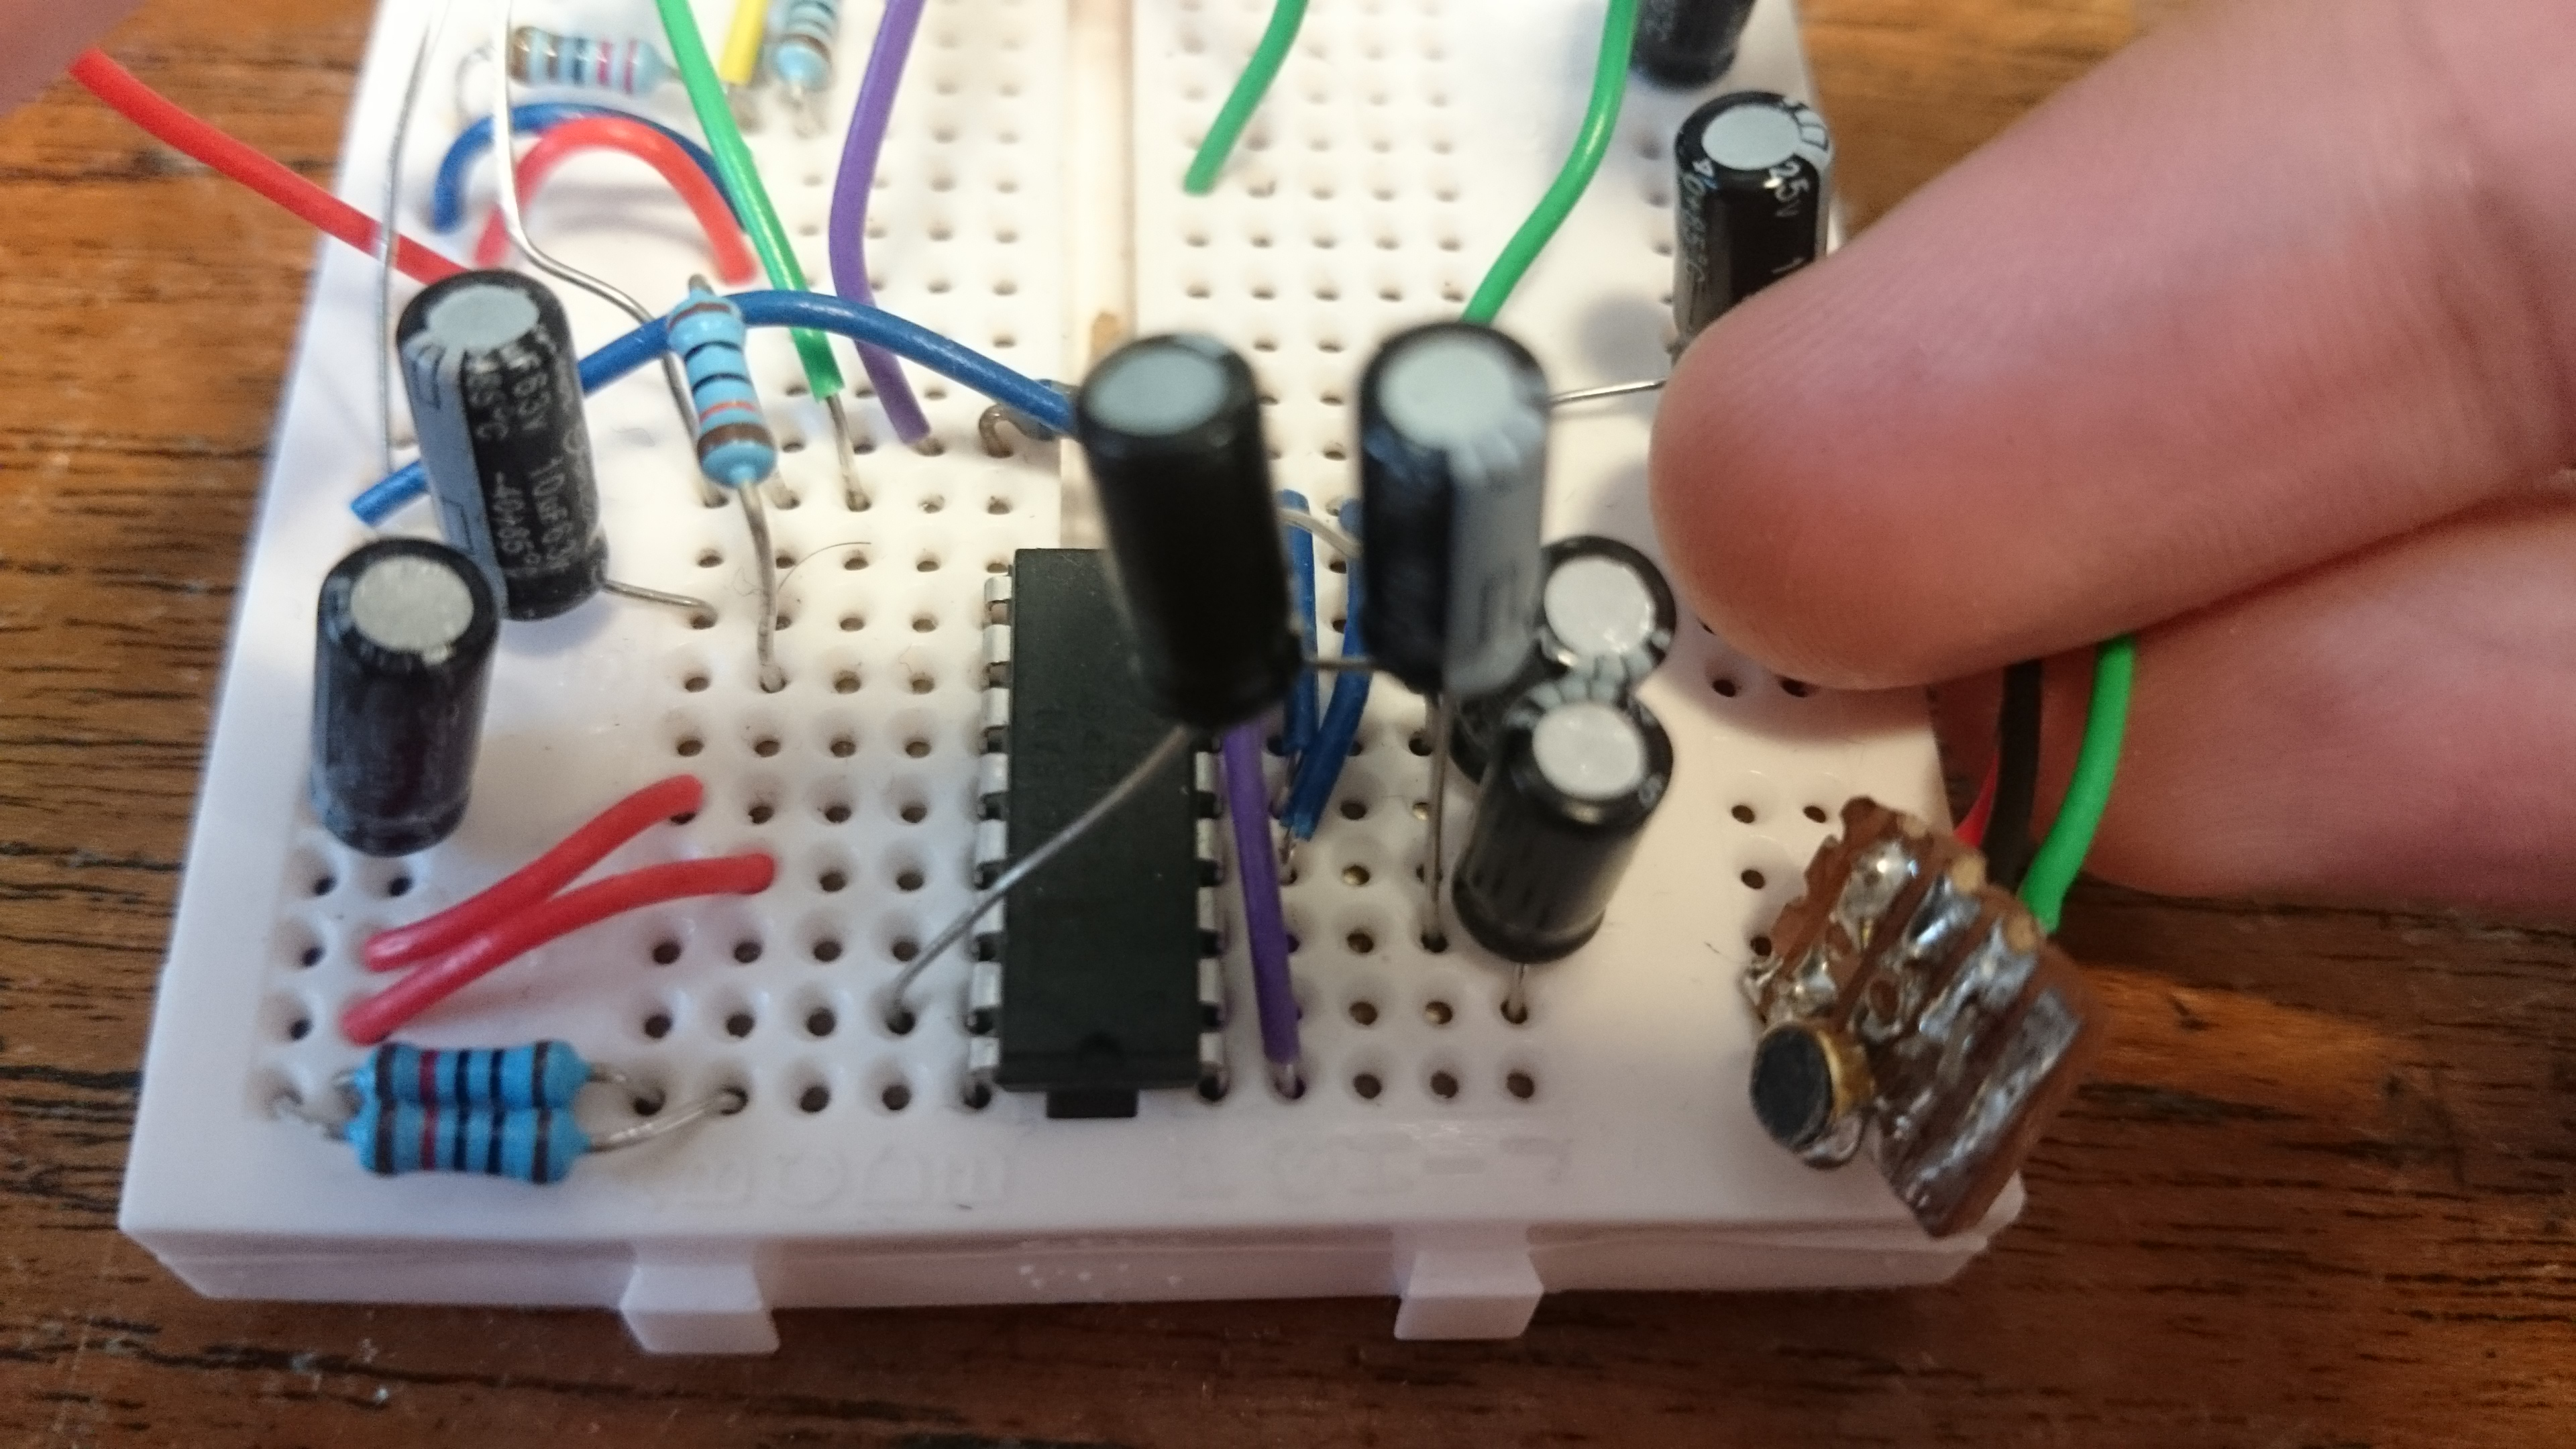
\includegraphics[scale = 0.05]{Images/ad605_circuit2}
\label{fig:veromic}
}
\caption{Programmable Gain Amplifier Circuit implemented on Breadboard, Prototype 0.1.03}
\label{fig:ad605}
%\end{figure}
\end{wrapfigure}

To set the gain of the AD605 once its circuit had been designed, the Arduino was to be programmed to output an analogue voltage. However, the Arduino Uno that I was using could only output Pulse-Width-Modulated (PWM) signals, meaning that the amplifier was receiving pulses of 5V and 0V rather than a particular constant voltage. In order to fix this, the PWM signal from the Arduino was low pass filtered\textsuperscript{\cite{pwmanalog}} with a series resistance of 68k$\Omega$ and a 10$\mu$F capacitor to ground, to obtain a DC voltage from the Arduino's 490Hz PWM signal. This voltage could then be set between 1.25 and 2.5V, which would correspond to gains of 0dB and 96dB respectively, by assigning a number between 63 and 127 to the relevant output pin on the Arduino. Setting the Gain Voltage Signal to zero would turn the amplifier off. 

Appendix~\ref{fingerboardsch} shows the full circuit diagram for a later Prototype but includes the pin connections for the AD605 chip to implement the discussed circuit with all decoupling capacitors, output lowpass filter and PWM-Analogue filter. The diagram also shows a potential divider connected to the Voltage Reference pin using two 10k$\Omega$ resistors to give the 20dB/V scaling that mapped the Gain Voltage Signal to the applied gain of the amplifier. After implementing this circuit, I decided to use it instead of the improved TL072 amplifier since it gave me the ability to control the gain digitally through the Arduino. 

\subsubsection{Improving the Arduino Code}

The Arduino's code for reading samples and writing them to the Serial bus was also modified. Instead of using a circular buffer, which introduced redundancies due to differences in its reading and writing speeds, an endless loop was written to iteratively read a single sample value and write it to the Serial bus. With this method, the input sample rate was considerably hampered by the function that printed the sample value to the Serial bus because another sample could not be read until the previous had been written. However, this method did remove the possibility of inaccuracies in the transmission of data such as repeated or lost sample values. 

\subsubsection{Microphone Circuit on Veroboard}

I isolated the microphone circuit onto a small piece of Veroboard, as can be seen in Figure~\ref{fig:veromic}. This allowed me to quickly plug the microphone into whichever amplifier circuit I was testing and I would also be able to emulate the final usage of the microphone by removing it from the breadboard and having the ability to move it around with my fingers.

%%%%%%%%%%%%%%%%%%%%%%%%%%%
\newpage
\subsection{Prototype 0.2.01} \label{0201}

Prototype 0.2.01 involved a significant development in the software Interface as I shifted from coding in Python to C++. This was after finding that the signal from the microphone was glitching when attempting to play it out of the speakers and this was due to code redundancies in the \textit{PyO} library for audio playback. Essentially, I realised that as much as I developed the User Interface, the audio output would simply not be as clean as I would like it to be, and the best way forward would be to switch over to C++ as soon as possible as it provided a much more efficient way of programming despite the fact that I would have to find new libraries and methods for implementing what I already had in Python. 

\subsubsection{New Program using JUCE in C++}

I found a library called JUCE\textsuperscript{\cite{juce}} which was designed to code audio-based applications in C++. Introjucer\textsuperscript{\cite{introjucer}}, a program for instantiating a JUCE application, provided me with skeleton code and allowed me to create GUI elements as classes which I could run from the main application. The skeleton code automatically generated two running threads: one to process audio samples based on a hidden recurring timer, and one to listen for events in the GUI. The interfacing of the application with my computer's audio device was hidden and I simply had to write code to provide the program with audio samples upon request. 

I used Introjucer to develop two GUI classes to run under the main application: an 'Overlay' class to show the 'Add Board' and 'Remove Board' buttons as before, and a 'Board' class to display the controls for selecting a serial port and the required mode. The main application would instantiate a single 'Overlay' object, which would then spawn as many 'Board' objects as required. This in fact allowed me to integrate the virtual Bus functionality from Python into the Board class, to process audio and display the GUI elements all from the same class. Figure~\ref{fig:0201UML} shows a class diagram of the structure of the Interface program and a summary of each class. Each 'Board' object was responsible for connecting to a selected serial port, storing received samples in a temporary Queue and then generating samples for the separate Voice and Sample buffers accordingly. The reason for this was that the Sample buffer need only store the loaded sample sound file, which would be played when the Queue was processed for 'triggers', and the Voice buffer, as described in the next Prototype, would need to store an upsampled version of the Queued signal because of the difference in the Arduino's sample rate and the required output rate of the audio device. 

\begin{figure}[H]
\centering
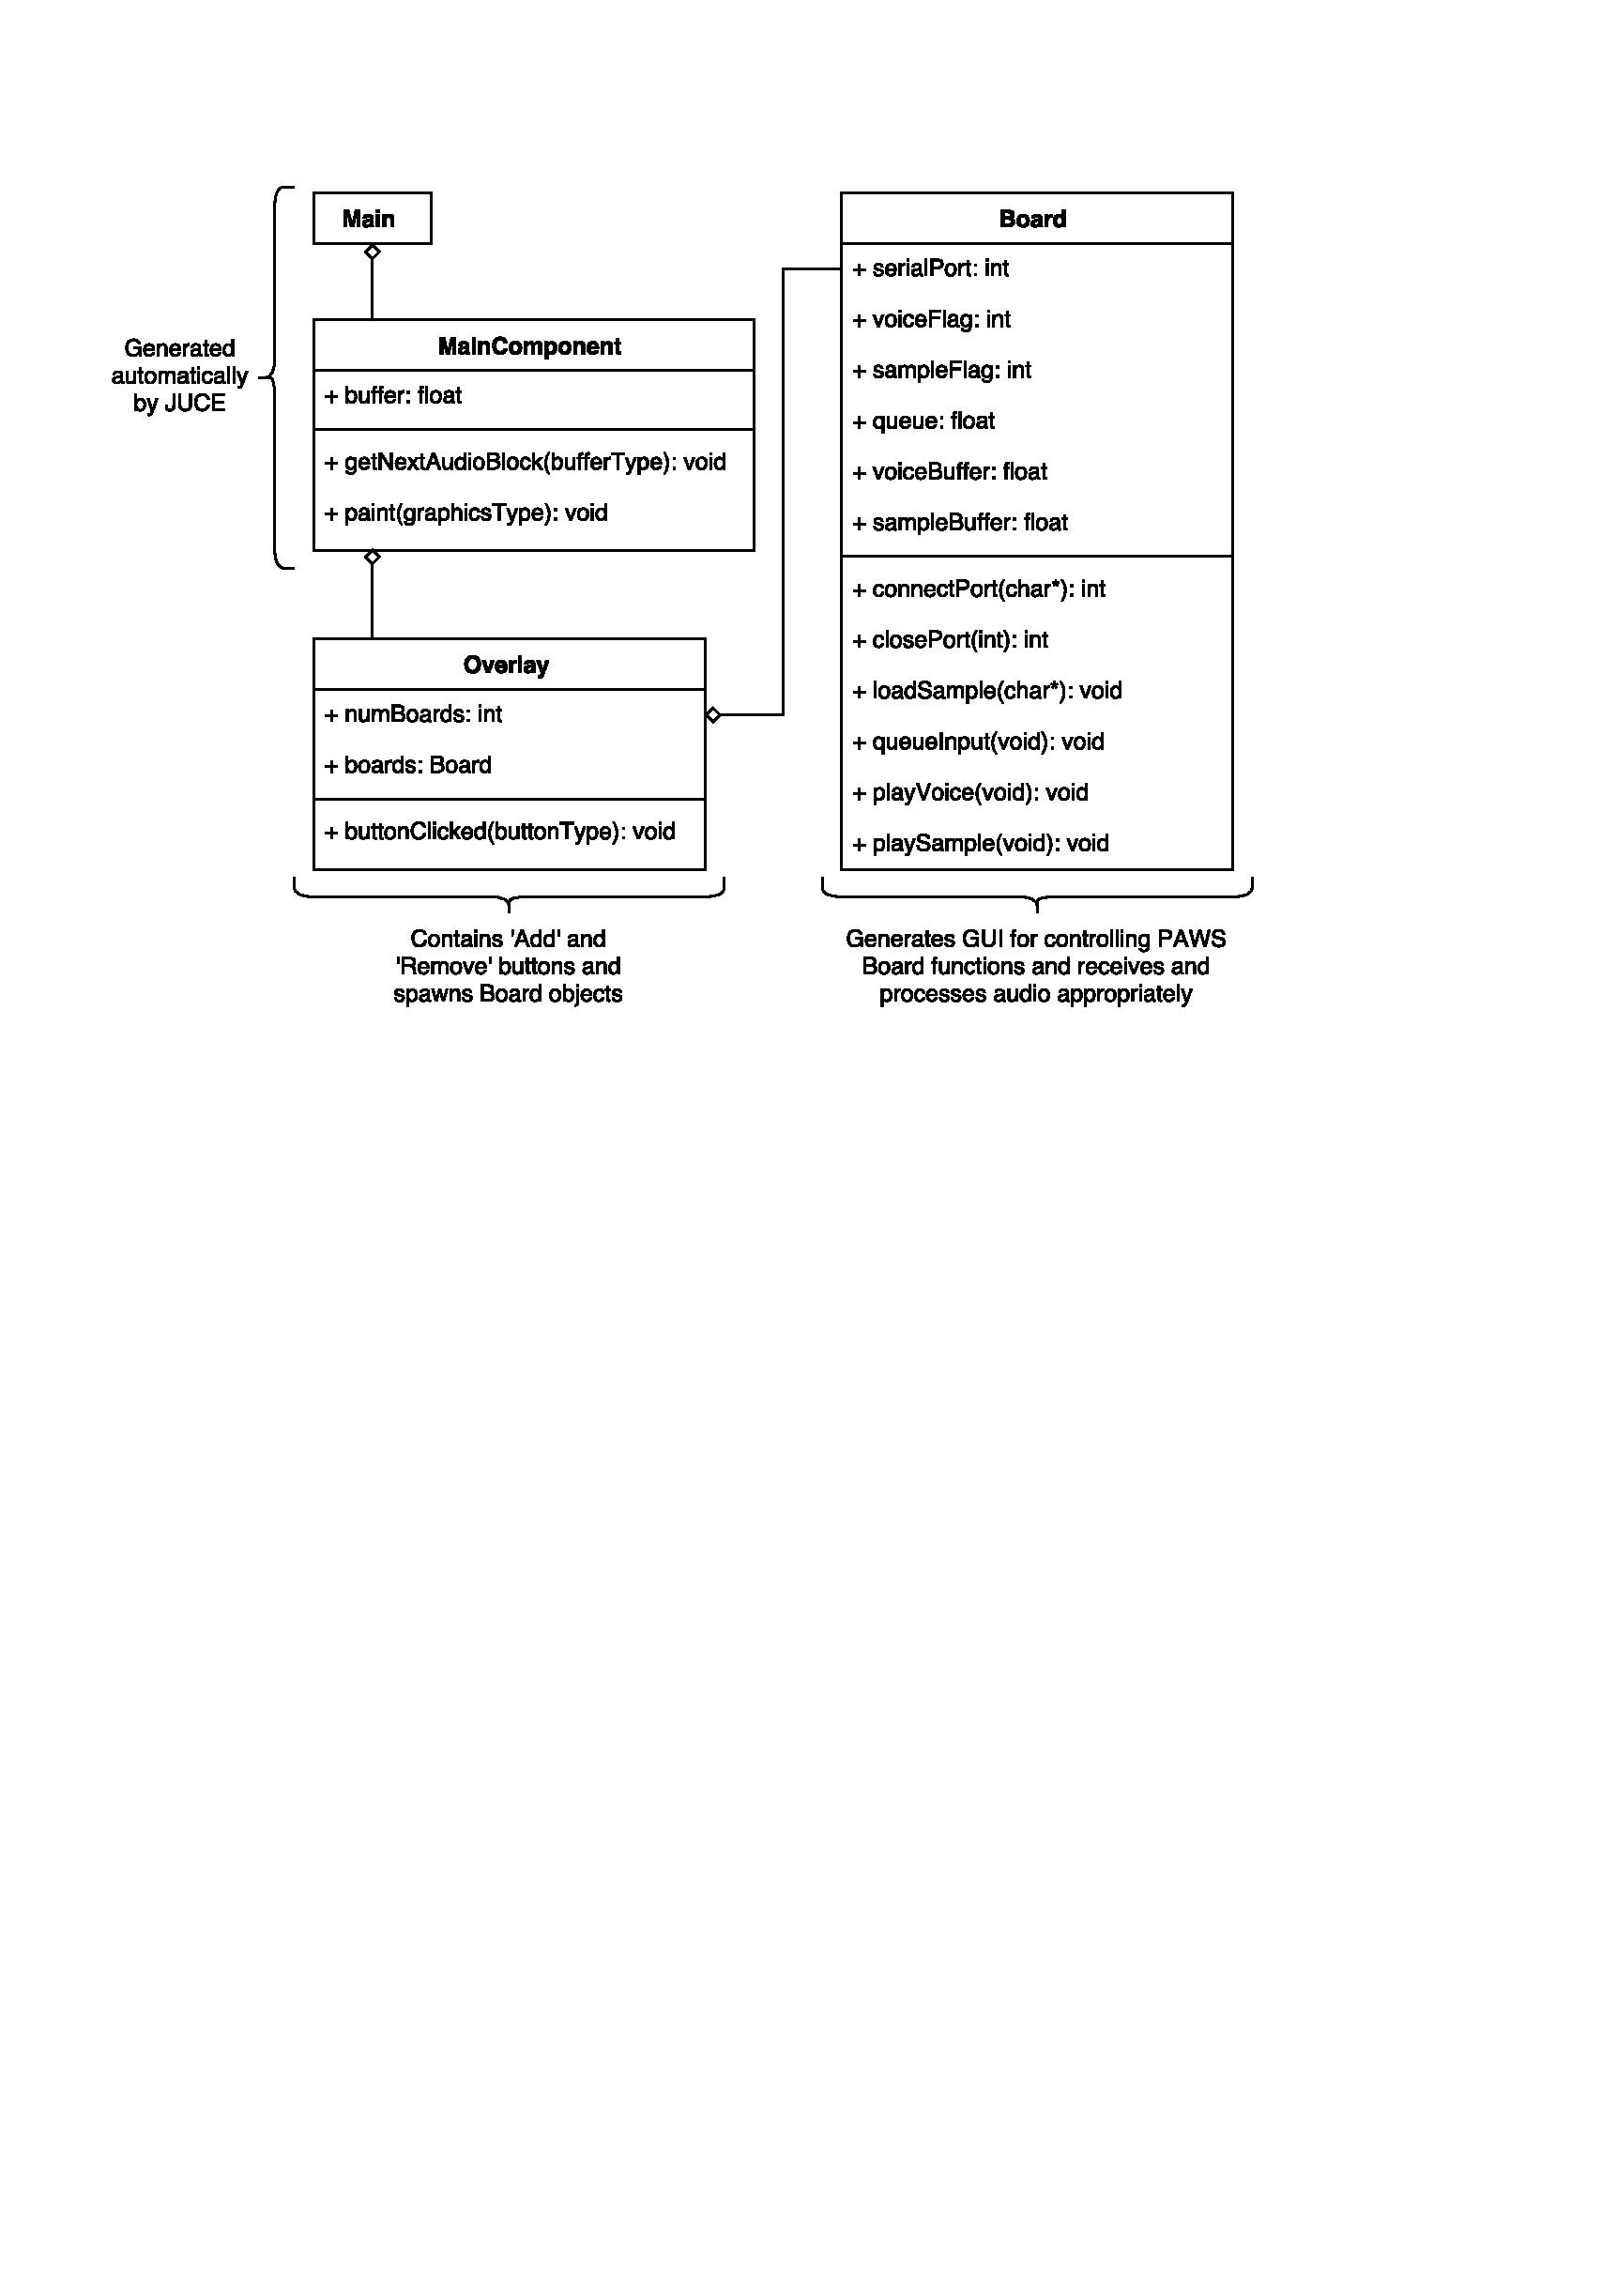
\includegraphics[scale=0.65]{Images/0201UML}
\caption{Class Diagram of Interface using JUCE, Prototype 0.2.01}
\label{fig:0201UML}
\end{figure}

\newpage

\begin{wrapfigure}[28]{r}{0.4\textheight}
\centering
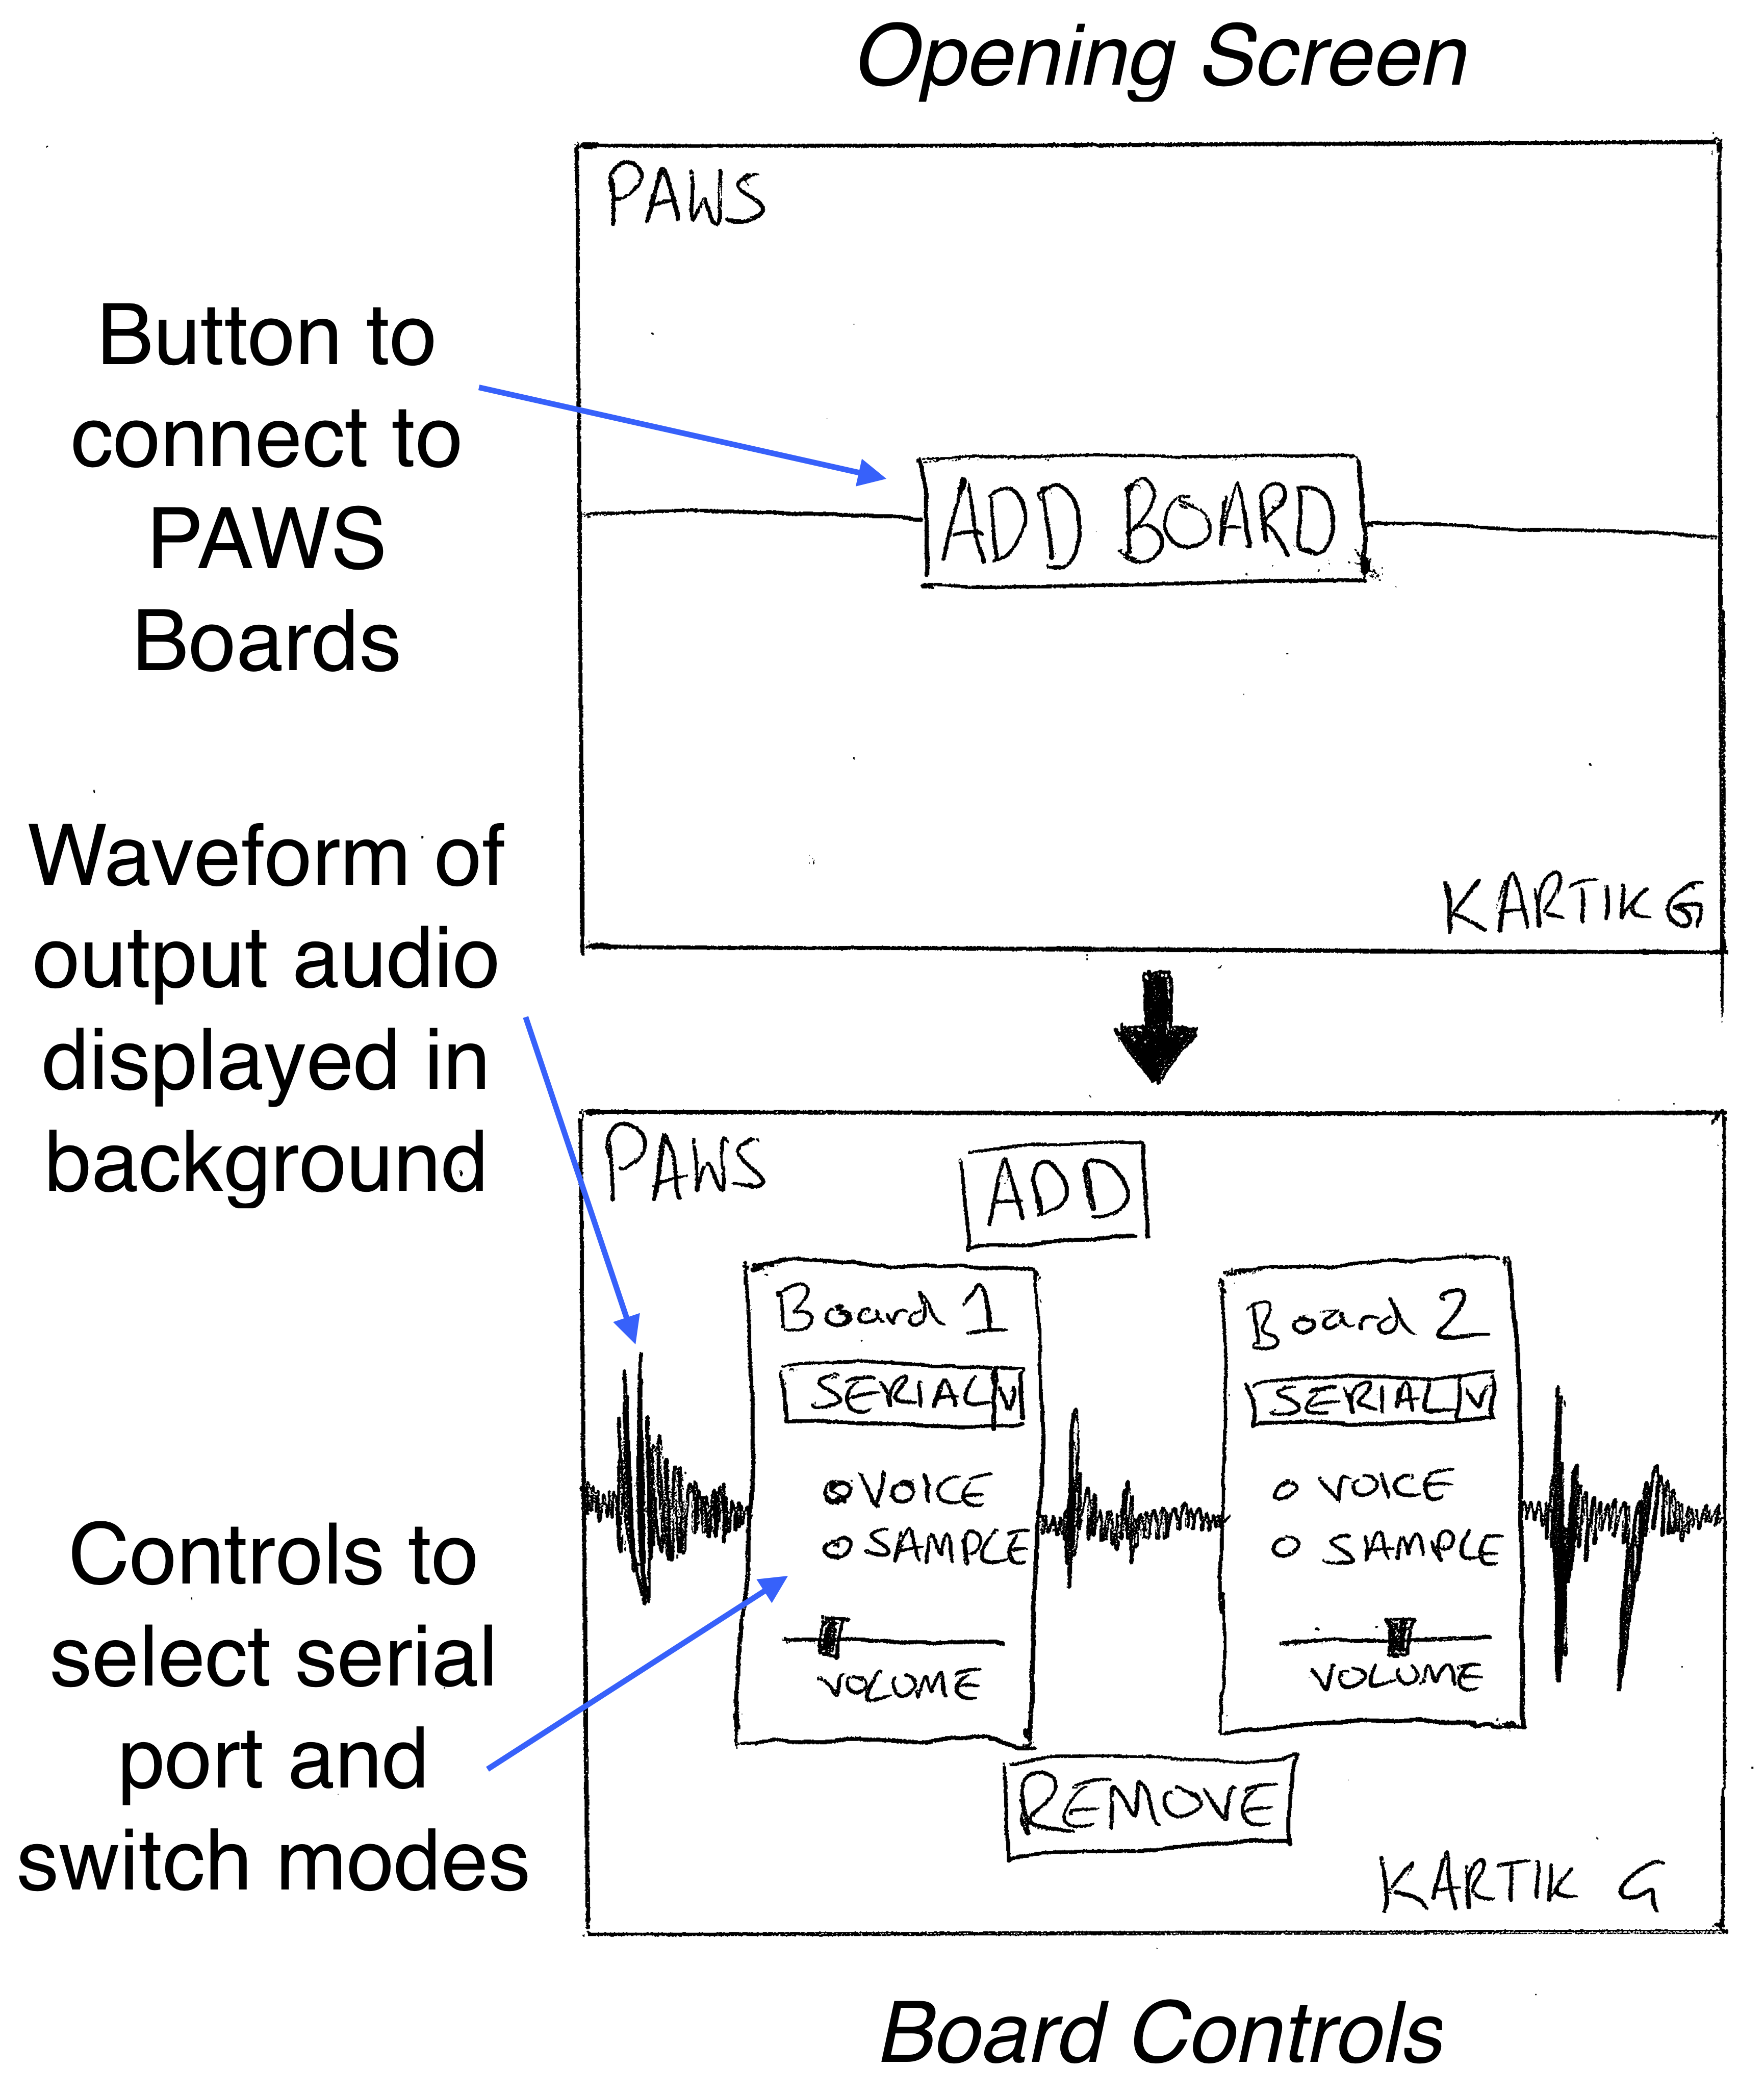
\includegraphics[scale=0.9]{Images/JuceConcept2}
\caption{Concept Sketches for JUCE GUI, Prototype 0.2.01}
\label{fig:juceguisketches}
\end{wrapfigure}

Appendix~\ref{juceflow} shows a flow diagram of the \textit{getNextAudioBlock(~)} in the JUCE application, which controlled the transfer of audio data from the temporary storage Buffers to the output audio device. Like the Python program shown in Appendix~\ref{pyblue_flow} it still utilised threading (using the C++ library \textit{pthread}\textsuperscript{\cite{pthread}}) to call the 'Voice' and 'Sample' functions, only this time the received audio samples were pulled into the main application's audio request thread, using the algorithm described by the flow diagram, and pushed into the audio device from there. 

\subsubsection{Designing the GUI}



Figure~\ref{fig:juceguisketches} shows concept sketches for the JUCE GUI. Upon startup, the application would show only the 'Add Board' button, as with the Python GUI. However, Introjucer allowed for the creation of a much more user-friendly GUI through simple modern designs. When a new Board was added, the 'Add Board' button would shift to the top of the screen and the centre would be populated by a box with all the necessary controls, such as selecting the serial port and mode, as defined by the 'Board' class. The 'Remove Board' button would then also appear below the 'Board' object. The addition of more Boards would result in more of these objects being spawned and they would collectively be centred on the screen. 

%\begin{figure}[H]
\begin{wrapfigure}{r}{0.43\textheight}
\centering
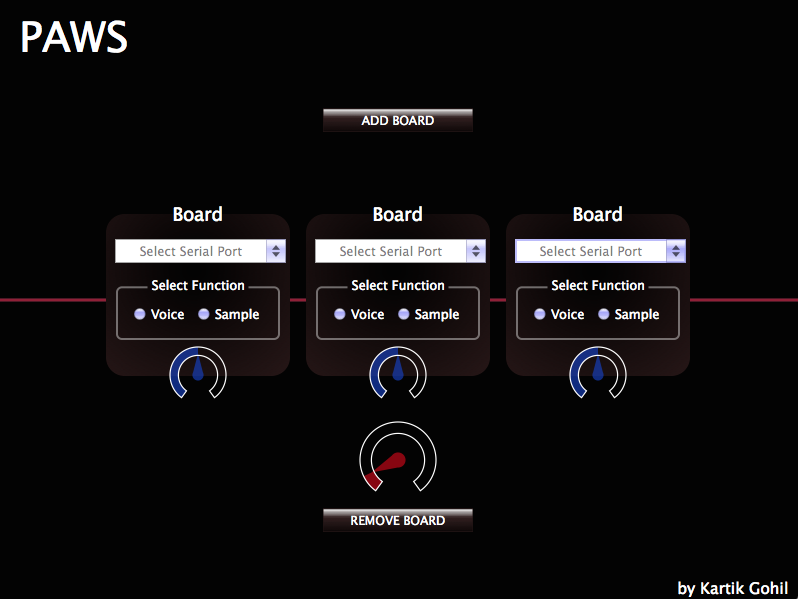
\includegraphics[scale = 0.35]{Images/paws_1_3}
\caption{Controls for 3 Boards in Interface, Prototype 0.2.01}
\label{fig:paws_3boards}
\end{wrapfigure}
%\end{figure}

The main application continuously runs a \textit{paint(~)} function to re-generate the background of the main frame as part of its GUI management thread. I exploited this function to display a waveform of the audio signal being processed by painting the the \textit{buffer} variable of the 'Main Component' class as shown in Figure~\ref{fig:0201UML} behind the 'Board' objects. This would provide visual feedback of the time-domain signal being sent to the audio device. Since the output signal was stereo or dual-channel (even though the microphone signal from my Boards were in mono or single-channel), I decided to overlay the Left and Right signals in red and blue respectively, which would show up as separate signals if the channels were different but would appear as a combined purple waveform if they were the same. This red and blue theme was used for the colour scheme of the entire application.

As an extra addition, volume controls were added to both 'Board' and 'Overlay classes, the former to set the gains of each individual Board, and the latter as a global amplitude control. These were also coloured in red and blue and were visualised as rotary faders to mimic what one would find on an audio mixing desk or professional studio equipment. Figure~\ref{fig:paws_3boards} shows the produced GUI with controls for three Boards and the waveform in the background shows the signal being received by one of the 'Board' objects connected to the Arduino in 'Voice' mode. 



\subsection{Prototype 0.2.02} \label{0202}

\subsubsection{Serial Communication and Bluetooth}

In order to connect to the Arduino using serial communication, I used a C++ library called \textit{termios}\textsuperscript{\cite{termios}}. This library allowed me to connect to a serial port and read data as was done in Python. I was not able to find a solution to detect available ports for dynamically updating the 'Select Serial Port' drop down list in the 'Board' class, and therefore had to pre-specify the Arduino's port until a solution could be found.

I found that if my computer was paired with the HC-06 Bluetooth module, it could be connected to as a serial device. After ensuring that I was able to read in values accurately through the USB cable, I attempted to test connecting to the Bluetooth module. Connecting to the HC-06 was straightforward enough but I found that the module itself was affecting the microphone circuitry. The power rails were being distorted by a steady square wave, most likely due to the Bluetooth module's change in power consumption as it pooled and transmitted data. 

\begin{wrapfigure}[19]{r}{0.45\textheight}
\centering
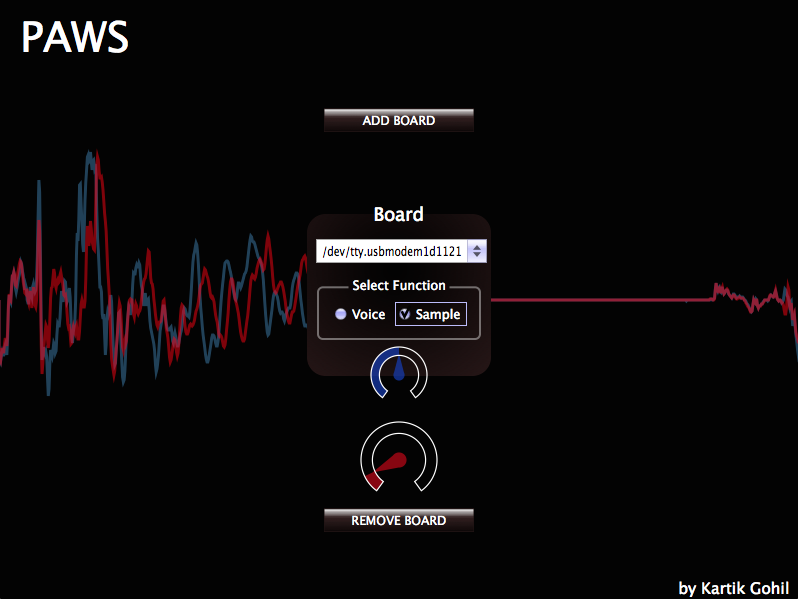
\includegraphics[scale=0.35]{Images/paws_1_sample}
\caption{Board connected to Interface in 'Sample' mode, Prototype 0.2.02}
\label{fig:paws_sample}
\end{wrapfigure}

Due to this, I stuck to using the USB cable for data transmission as I could also use it to power my arduino and microphone circuit. An independent power source for the microphone circuit would be ideal as the power drawn from the computer was corrupted with digital noise and the Arduino only seemed to add to that, but this solution worked for the time being and was in fact more reliable than communication via Bluetooth. 


\subsubsection{Implementing the 'Sample' Mode}

I was able to program a function to read a sample sound file, for example that of a drum hit, into a buffer but I had to rethink the way the function would trigger the sound because of the architecture of the JUCE program. The top-most 'Main Component' class called a function \textit{getNextAudioBlock(~)} to read the sample values stored in the buffer of each 'Board' object, which was of course being populated by the 'Voice' function receiving data from the Arduino. This function also requested 512 data samples with each call, and therefore my code for 'Sample' mode had to take this into account when trying to play a sound file consisting of tens of thousands of data samples. 

In order to implement the 'Sample' function, I used flags to determine whether a peak in the input audio signal had been detected, and the \textit{getNextAudioBlock(~)} would check these flags and pull the drum sound samples from a separate sample sound buffer. This meant a lot of processing was involved to ensure that only 512 samples of the drum sound were pulled at a time and that the position of the next samples to be played was recorded. I also enabled the function to reset the next data sample to be pulled if another 'tap' was detected during playback, so as to improve its responsiveness. This meant that the previous drum sound being played would be cut short rather than overlaid onto the new sound but it would react better to the user's performance.

All in all, it took some time to implement this function but I was able to play a sample drum sound by detecting peaks in the input signal from the Arduino. Figure~\ref{fig:paws_sample} shows a screenshot of the GUI during a sample being triggered by a 'tap' on the microphone. However, since the peaks in the microphone signal did not necessarily represent 'taps' and could in fact be artefacts of speech or even noise, I found that the function misfired, or played drum sounds when it was not supposed to. Filtering the input signal was considered to ensure that only the sound of tapping a surface was being processed for peak detection. 


\subsubsection{Upsampling for the 'Voice' Mode}

As discussed previously, the Arduino read a data sample and wrote it to the Serial bus as quickly as it possibly could. The Arduino Uno's \textit{analogRead(~)} function was rated at being able to read 10,000 samples per second (i.e. a 10kHz sample rate) but since the function that printed values to the Serial bus was so processor intensive, the effective sample rate was in fact much lower. 

\begin{wrapfigure}{r}{0.45\textheight}
\centering
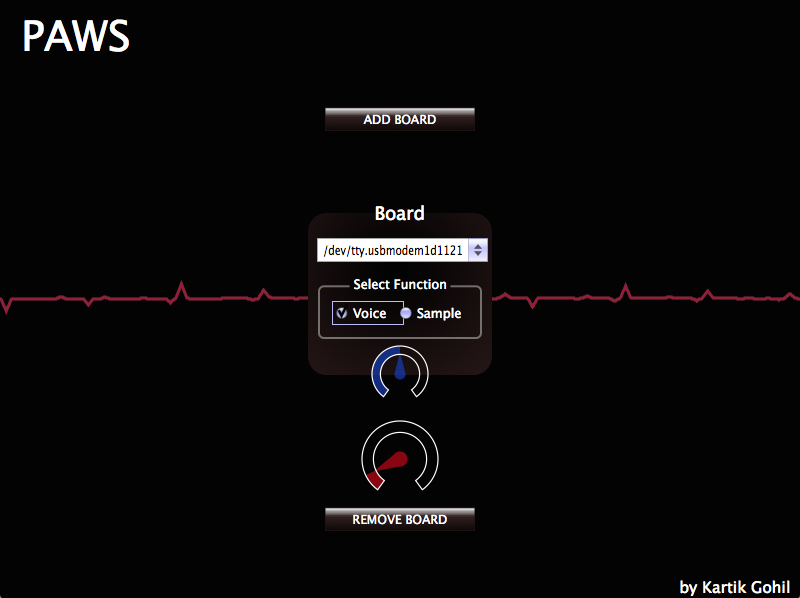
\includegraphics[scale=0.35]{Images/paws_1_voice}
\caption{Board connected to Interface in 'Voice' mode, Prototype 0.2.02}
\label{fig:paws_voice}
\end{wrapfigure}


Thus, when we read samples in to the Interface on the computer, and outputted them at the JUCE library's preset rate of 44.1kHz, we could not hear the audio signal correctly. In order to remedy this change in sample rate, we needed to upsample the signal to 44.1kHz. I used linear interpolation to perform the upsampling, whereby new samples were created in between two read samples to formed a linear ramp from the first sample to the last. This increased the number of samples representing a particular time period (the sample rate) while maintaining the waveform to some degree of accuracy. 


When outputting the input samples without any upsampling, I found that the input sample rate was approximately 13 times smaller than 44.1kHz. This was determined by calculating that every time the \textit{getNextAudioBlock(~)} function requested 512 samples, the program had in fact only read in about 39 samples from the Arduino. Therefore the input signal was interpolated by a factor of 13, that is, twelve new sample values were created and stored in between any two input values in such a way as to form a linear change between them.

By doing this, the output signal was able to produce the correct frequencies and my voice could be heard at the correct pitch, if a bit unclear. The signal was found to be fairly distorted and fuzzy, which I determined to be digital noise as well as the initial low sampling rate of the Arduino. 

\subsubsection{Coding the Serial Transmission}

I attempted to code the serial transmission in order to improve the speed at which samples were written to the Serial bus by the Arduino, and thereby reduce the time spent between reading samples.

I maximised the transmission baud rate to 230400 to ensure that data was sent as quickly as possible between the Arduino and the Interface. I was using a \textit{print line} function to print the sample values to the Serial bus followed by a 'new line' character to separate each value. However, I realised that this function was first converting the integer values into a string of characters, where each character was an ASCII representation of a digit, and then transmitting it. This meant that an integer of size two bytes (16 bits) was being transmitted as a maximum of five bytes: a maximum of four to represent each of the digits in the range 0 to 1024, and a final byte for the 'new line' character.

I removed this redundancy by simply writing the two bytes of the integer value directly to the Serial bus, followed by the 'new line' character, thereby reducing a variable transmission rate of three to five bytes of data to a constant three bytes per sample. I realised that the \textit{analogRead(~)} function only produced a 10 bit value, to give the range 0 to 1024, and therefore only occupied a fraction of the upper byte of an integer value. In order to reduce the transmission rate even further, I divided each sample value by 4, to remove the lower 2 bits, and simply transmitted the first byte. The transmission rate was then lowered to a fixed two bytes per sample. 

The Interface was re-programmed to wait for a 'new line' character before reading in a byte of information, parsing it to an integer data type, and then multiplying it by 4 again, before saving it to the data buffer, which could later be called for upsampling. Another method for reducing the size of a sample from 10 bits to 8 bits was to simply shift all the bits along to the right by two and then taking the first byte to ensure the most significant bit (MSB) was captured. The bit shifting worked on the same principle as a division of 4 but it was found that the audio quality was somewhat clearer using the division, despite the two methods being absolutely identical in terms of function. This comparison was determined qualitatively and could have been utterly dependent on the differences between the signals being captured by the microphone. In any case, I stuck with the division by 4 method. 

\subsection{Prototype 0.2.03} \label{0203}

\begin{wrapfigure}[27]{r}{0.27\textheight}
\centering
\subfloat[Finger Board PCB]{
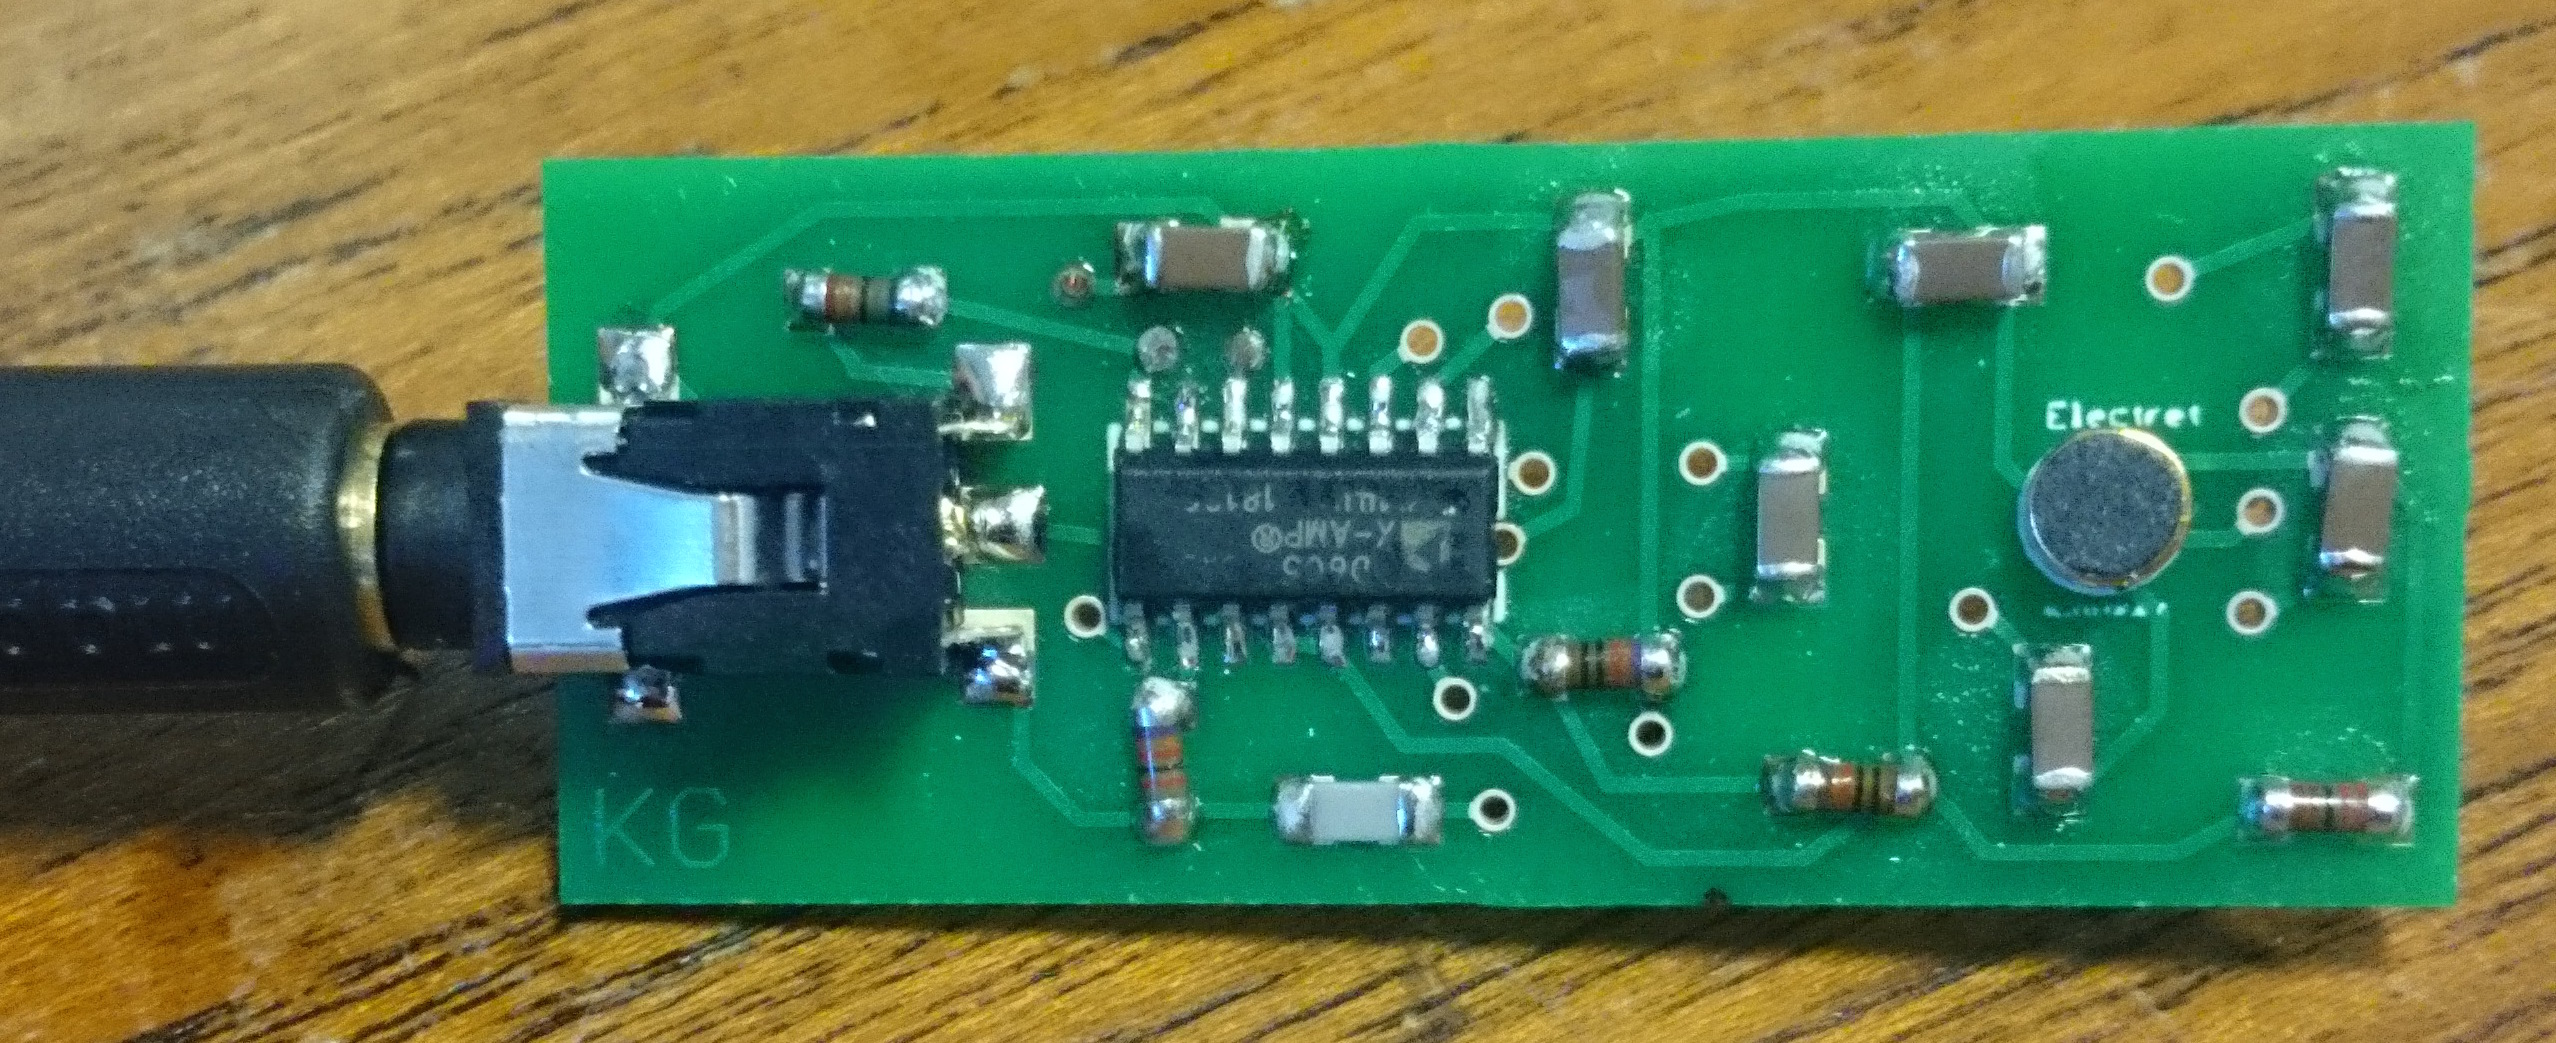
\includegraphics[scale=0.07]{Images/fingerboard_pcb}
}\\
\subfloat[Arduino Shield PCB]{
\includegraphics[scale=0.05]{Images/ardshield_pcb}
}
\caption{PCBs for PAWS Board, Prototype 0.2.03}
\label{fig:finalpcbs}
\end{wrapfigure}

With this prototype, I designed Printed Circuit Boards (PCBs) for the microphone circuitry and 3D printed housings in the shape of rings to allow a user to wear the microphone circuit on their finger. This design evolution implemented the microphone circuitry on a Finger Board and created an Arduino Shield to slot directly into the Arduino Uno, and these two PCBs alongside the Arduino formed a PAWS Board. 

\subsubsection{Hardware on Printed Circuit Boards}

I used a software tool called \textit{Eagle}\textsuperscript{\cite{eagle}} to design my circuits and generate layouts for PCBs. I designed two circuits: a Finger Board for the microphone circuitry which could physically be worn at your fingertips, and another as Shield to slot on top of the Arduino Uno. 

The Finger Board was designed to house the microphone circuit, along with the AD605 programmable gain amplifier. Since the circuitry would require a positive rail voltage from the Arduino of 5V, a ground voltage, and a signal to control the gain of the amplifier, a connector would be required to receive these voltages via a cable from the Arduino. A four way connector was chosen to account for the microphone signal being sent to the Arduino.  

The Arduino Shield was designed to be of the same size as the Arduino Uno with connections such that it could simply slot in place. It was designed to connect via a cable to not one but three Finger Boards, for such a time when the software was upgraded to be able to control three microphone inputs all at once. This functionality would preserve the ability to connect to and program multiple sensors independently despite there only being a single microcontroller. The circuitry for the HC-06 bluetooth module was also included just in case I wished to insert it in the future. 

Appendices~\ref{fingerboardsch} and \ref{ardshieldsch} show the drawn circuit schematics for Prototype 0.2.03. 

After drawing the circuit schematics, I designed the PCBs in terms of their size and the layout of all the components. I chose the components to be as small as possible while maintaining the ability to solder them myself. I used the same Kingstate Electret Microphones as before but I used a surface mount package for the AD605 chip, which happened to be slightly smaller than its Dual-Inline Package counterpart that I was testing on Breadboard. For the resistors and capacitors, I opted for the MELF0204 and C3216 packages respectively as they were also surface mountable but large enough to solder with my hands. I also chose to use a 4-way male-to-male 3.5mm jack audio cable to connect the Arduino Shield to the Finger Boards. This meant that the female connectors required by both Boards could be small as they featured concentric connection rings for the 4 signal paths, and I was also able to find them in a surface mountable package. 

For the Shield, I used Single-Inline male connectors to slot directly into the pin headers in the Arduino Uno. The jack cable connectors for the Shield were of course exactly the same as the ones for the Finger Boards. 

Appendices~\ref{fingerboardpcb} and \ref{ardshieldpcb} show the PCB layouts for each of these Boards and Figure~\ref{fig:finalpcbs} shows images of the final PCBs after soldering all the components down. 

The Arduino Shield was designed to connect to three Finger Boards and provide a separate gain voltage to each of their programmable amplifiers. This was designed to work with the current Interface, which could connect to the Arduino and access a single microphone, and with a future Interface, detailed in Subsection~\ref{0204}, to allow the user to control the functionality of three Finger Boards individually.



\subsubsection{3D Printed Finger Rings}

\begin{wrapfigure}[13]{r}{0.29\textheight}
\centering
\subfloat[Top View]{
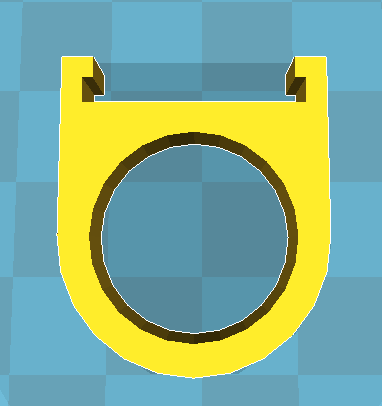
\includegraphics[scale=0.2]{Images/fngrbrdmod1_top}
}
\subfloat[Side View]{
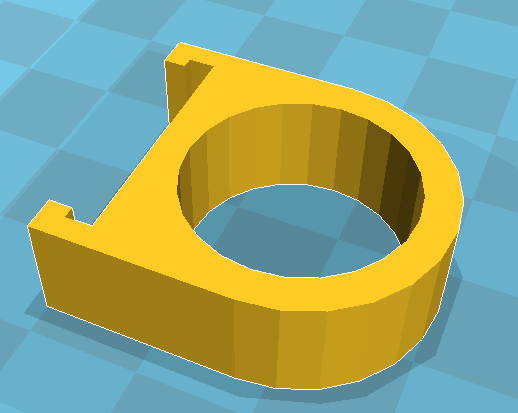
\includegraphics[scale=0.195]{Images/fngrbrdmod1_side}
}
\caption{Finger Ring 3D Model - Version 1, Prototype 0.2.03}
\label{fig:fngrbrd_1}
\end{wrapfigure}

To make the Finger Boards wearable, I required plastic housings that could be 3D printed. The design itself would have to consist of a ring to sit around the top knuckle and a support to hold the PCB in place. The measurements I took to design the ring were of the index finger of my right hand.

I used a free software called \textit{SketchUp}\textsuperscript{\cite{sketchup}} to design a model of a Ring to be printed later. The tool itself was easy to learn and the first version of the Ring, Figure~\ref{fig:fngrbrd_1}, was designed as a line sketch which was then extruded by 10mm to form a 3D model. 

Once the Ring had been designed, I used \textit{Cura}\textsuperscript{\cite{cura}} to detail how it would be printed using an \textit{Ultimaker 2}\textsuperscript{\cite{ultimaker}} 3D Printer. The tool allowed me to set the fill of the piece (i.e. hollow to solid) and the depth of each printed layer, which would determine the precision of the print. After setting all of the parameters, I was able to print the Ring.

With the first version, I found that I had overestimated the dimensions; the Ring was too large and slid all the way down to the bottom of my index finger, which is not where it should have been, and the support on the top did not hold the PCB in place at all. 

%\begin{figure}[H]
\begin{wrapfigure}[13]{r}{0.29\textheight}
\centering
\subfloat[Top View]{
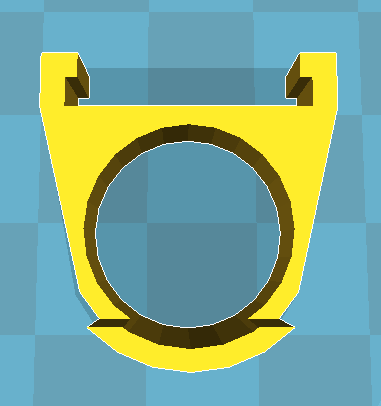
\includegraphics[scale=0.2]{Images/fngrbrdmod2_top}
}
\subfloat[Side View]{
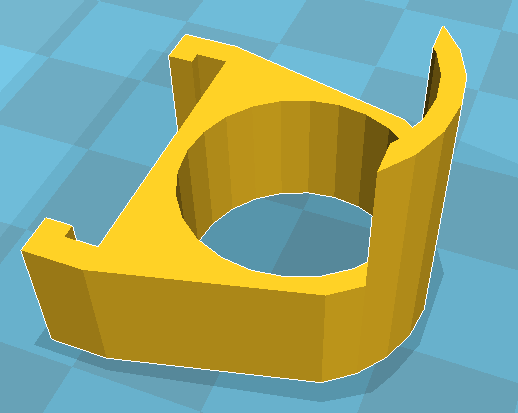
\includegraphics[scale=0.195]{Images/fngrbrdmod2_side}
}
\caption{Finger Ring 3D Model - Version 2, Prototype 0.2.03}
\label{fig:fngrbrd_2}
\end{wrapfigure}
%\end{figure}

I redetermined the measurements and designed a second version, shown in Figure~\ref{fig:fngrbrd_2}. This version was designed to have less of a curvature around the bottom to prevent it from being as bulky as the first version. I also added a 'lip' like feature to the bottom of the Ring, which would sit under the tip of the index finger and produce a loud tone when tapped against a surface. This design would in future help the Interface to better determine whether a surface was being tapped and therefore make the 'Sample' function a lot more robust. 


For the final batch of Rings, I realised that the lip from Version 2 had to be much wider in order to sit comfortably around the finger without digging into it. I also created another design with sizings to fit my thumb, which of course is slightly larger than my fingers. Figure~\ref{fig:fngrbrd_3} shows dimensioned sketches of the final produced batch of Rings, labelled as Version 3, with both Finger and Thumb variants. Figure~\ref{fig:fingerrings} shows an image of two Finger Rings and one Thumb Ring being worn.

\begin{figure}[H]
\centering
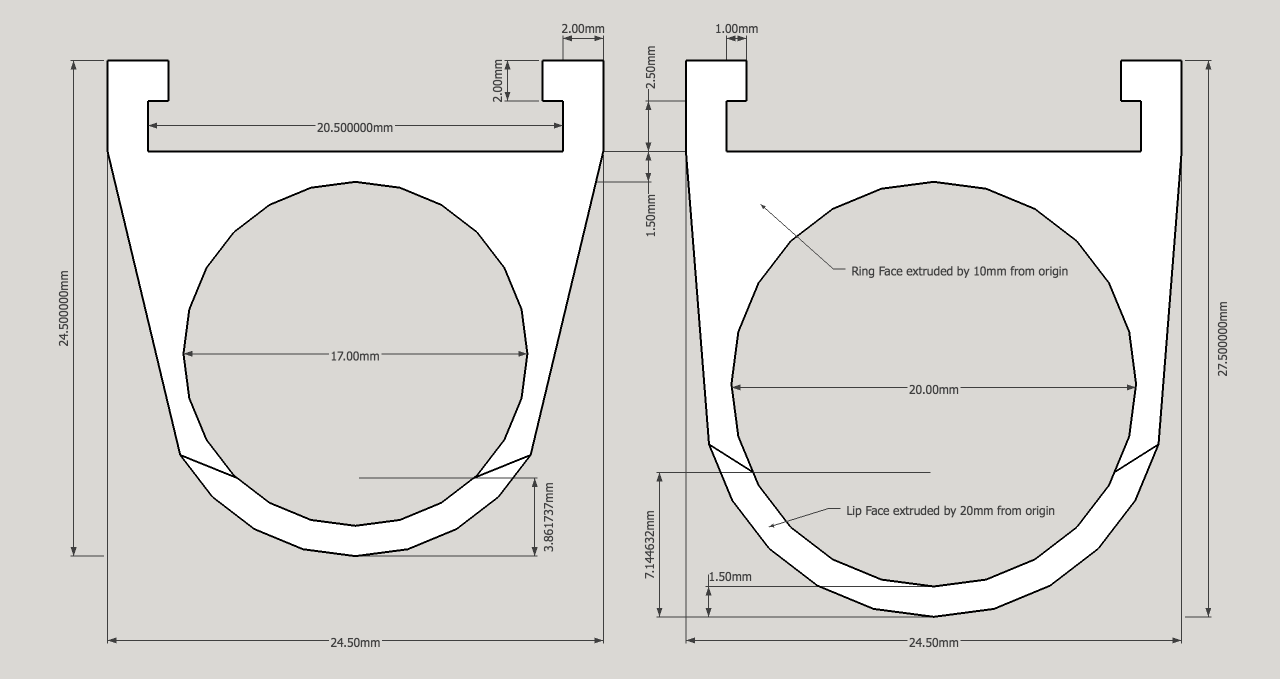
\includegraphics[scale=0.3]{Images/fngrbrdfinal_dim}
\caption{Dimensioned Sketches of Rings Version 3 - Finger (Left) and Thumb (Right), Prototype 0.2.03}
\label{fig:fngrbrd_3}
\end{figure}

\begin{figure}[H]
\centering
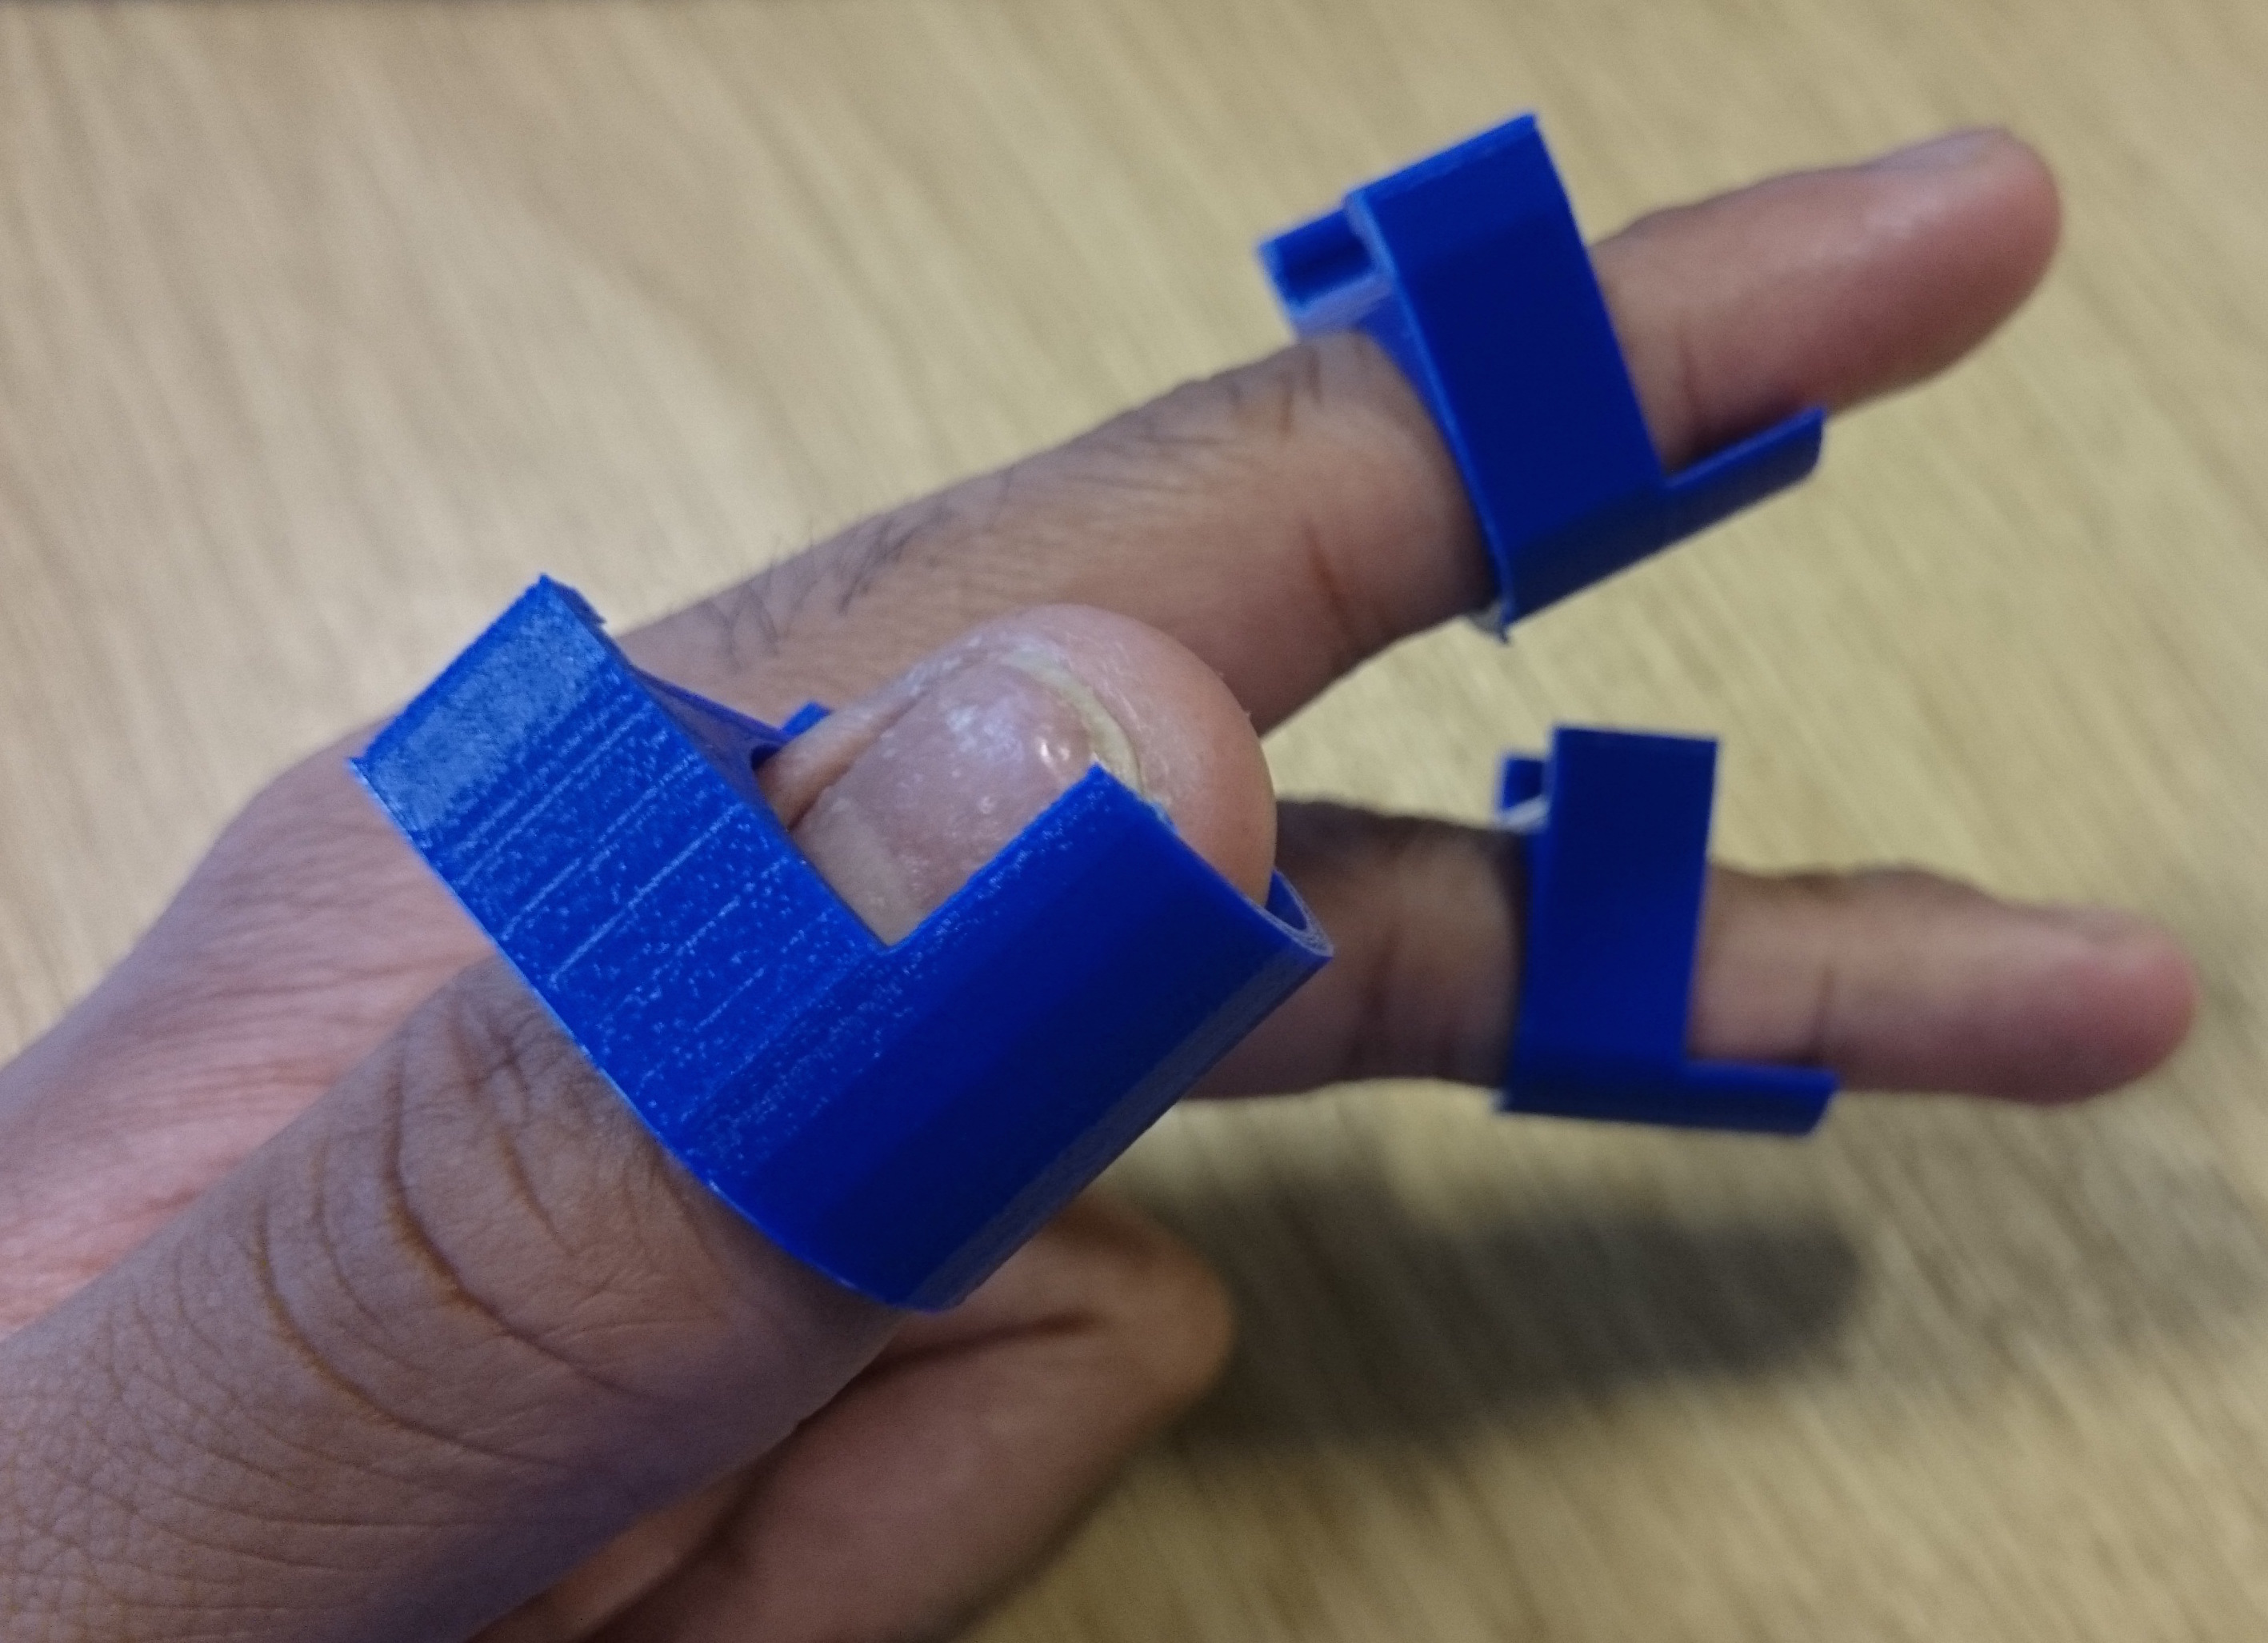
\includegraphics[scale=0.1]{Images/fingerrings_3}
\caption{1 Thumb Ring and 2 Finger Rings worn by a user, Prototype 0.2.03}
\label{fig:fingerrings}
\end{figure}

\newpage
\subsection{Prototype 0.2.04} \label{0204}

The previous prototypes had all been designed with the idea of connecting to PAWS Boards one by one, with each Board housing a single microphone. This prototype designed a new Interface for connecting to a single Arduino Uno that could control three different Finger Boards. The PCBs were previously designed to allow for this functionality and the Interface and Arduino code had to be modified slightly to connect to and control more than one Finger Board. 

\subsubsection{Connecting to multiple Finger Boards}

\begin{wrapfigure}{r}{0.3\textheight}
\centering
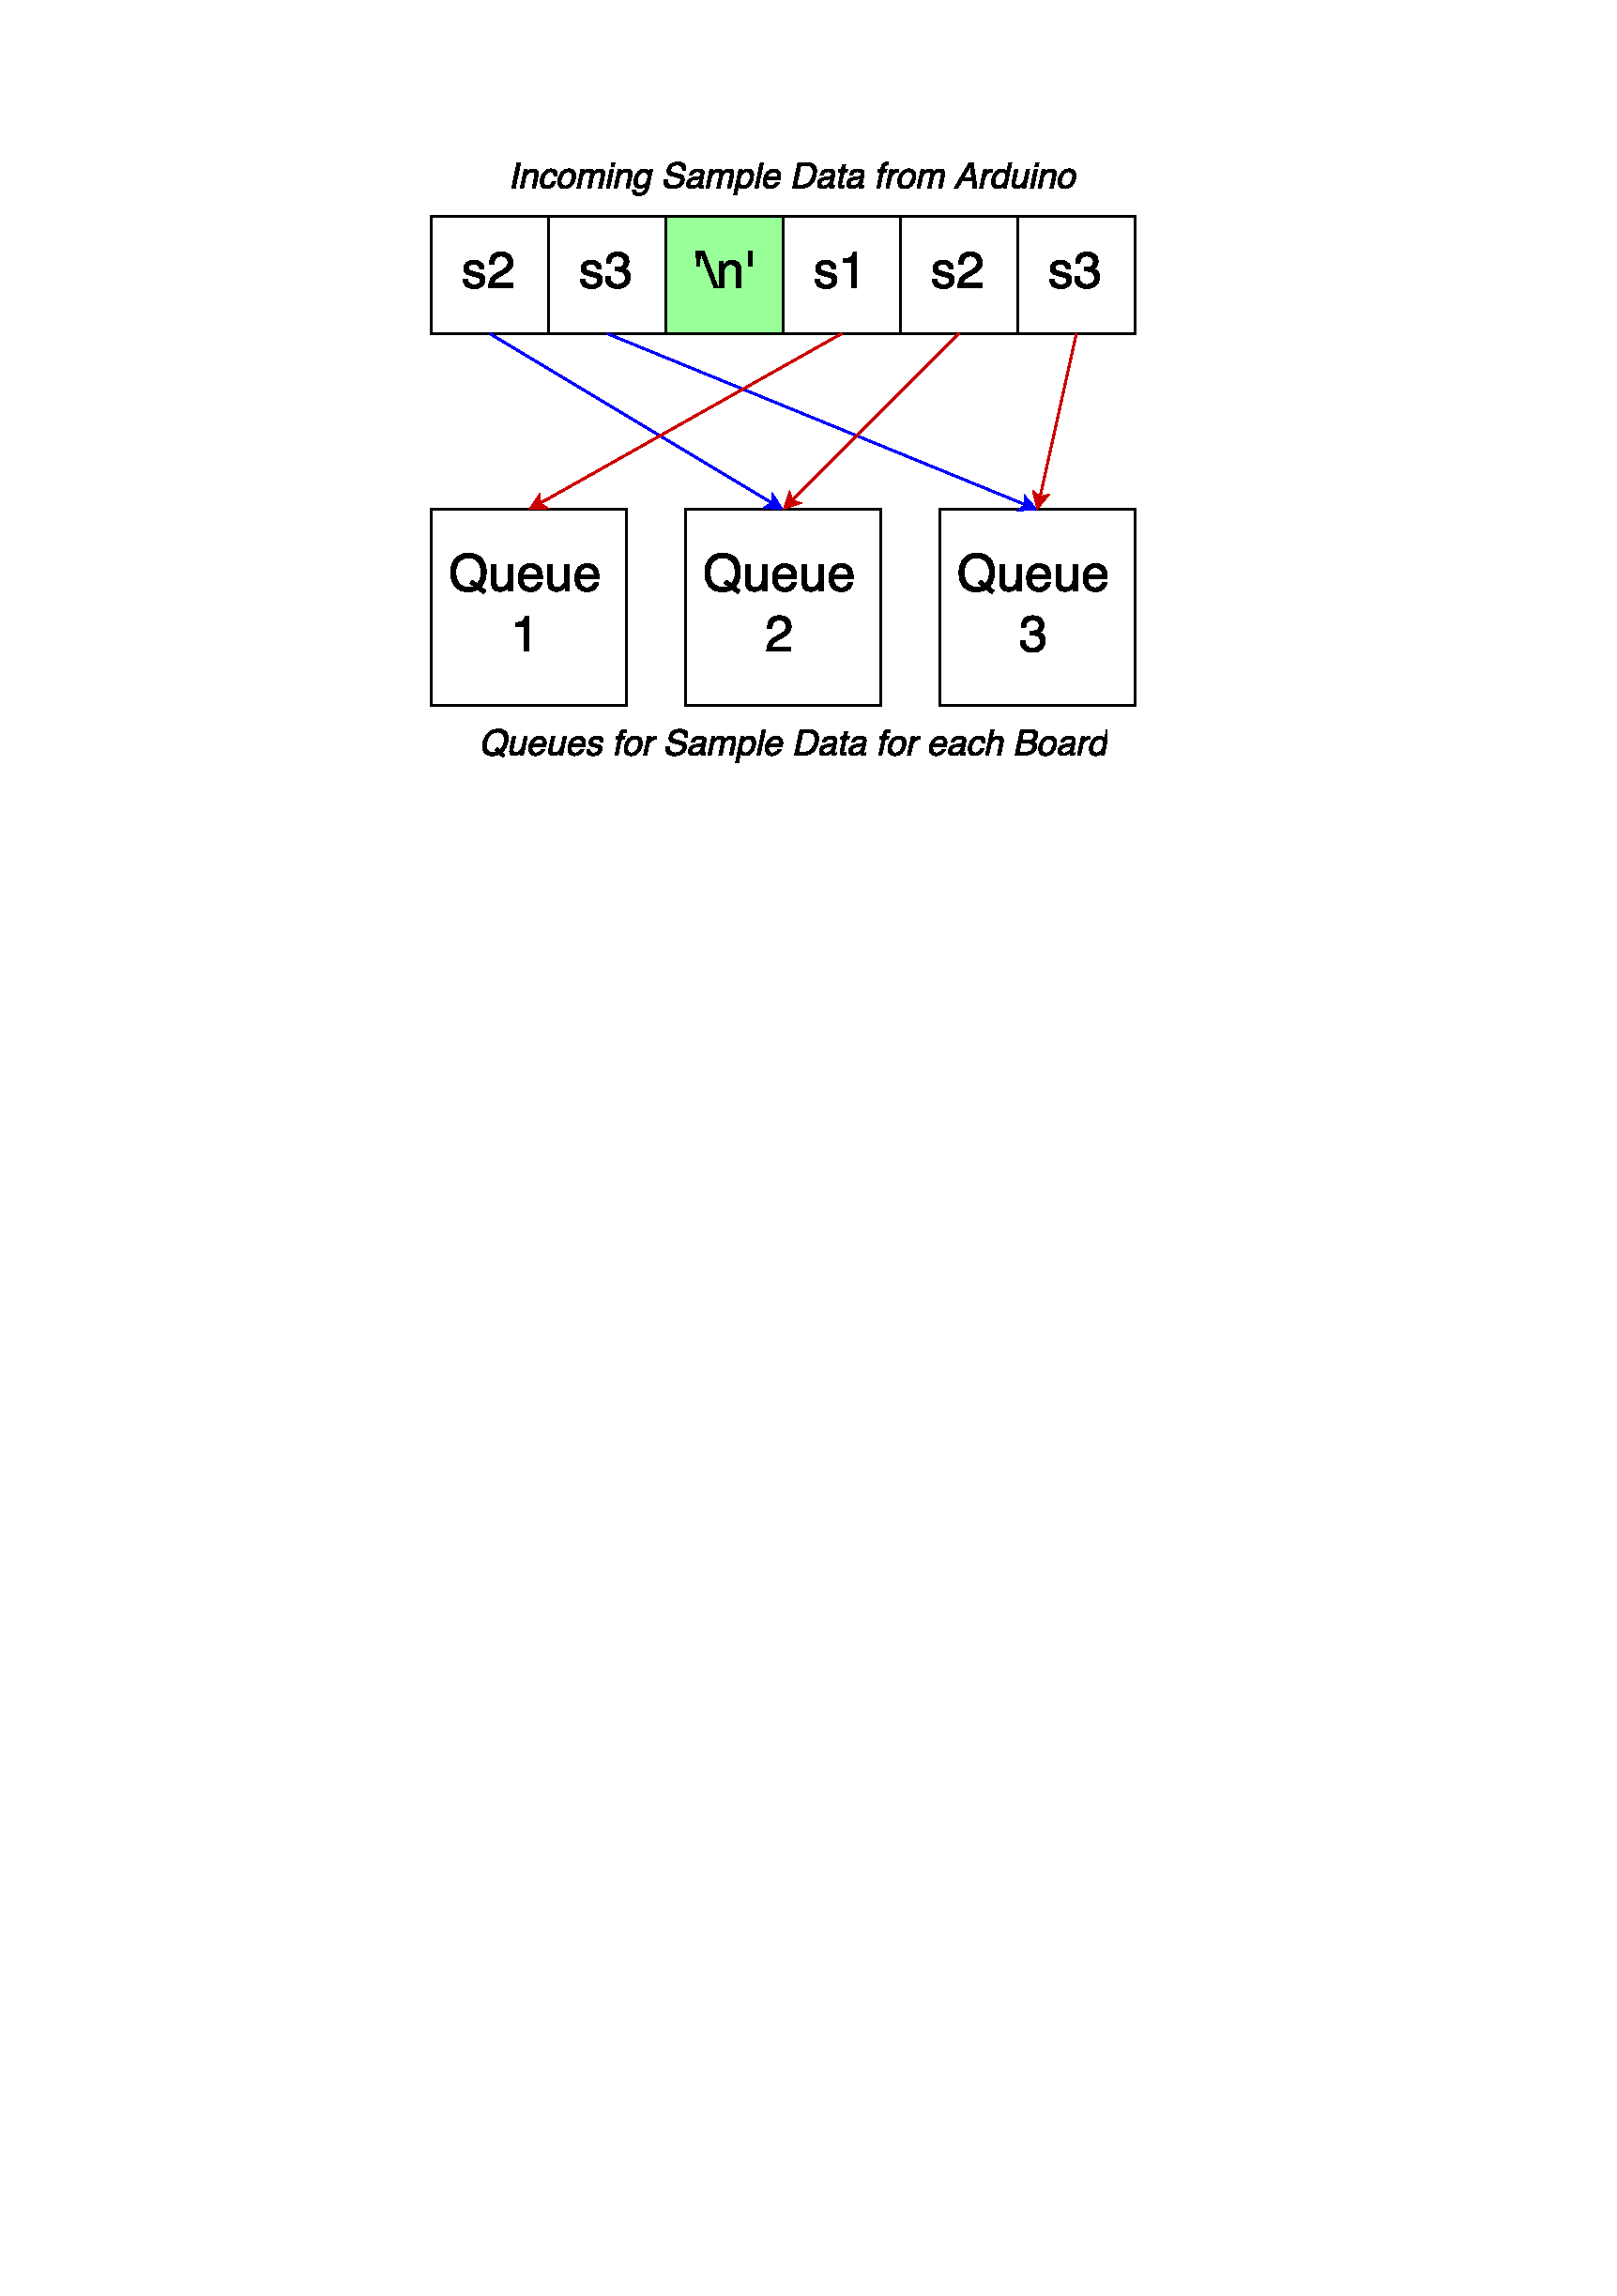
\includegraphics[scale = 0.5]{Images/sampleassignment}
\caption{Assignment of received sample data to the relevant Queue buffers by the Interface's \textit{queueInput(~)} function, Prototype 0.2.04}
\label{fig:sampassign}
\end{wrapfigure}

To allow the Interface to control each of the Finger Boards attached to the Arduino Uno separately, I had to make several changes to the functions of the two main classes that controlled the GUI. The \textit{Overlay} class was previously in charge of adding and removing 'Board' objects. For this prototype, I required the 'Overlay' class to perform the connection to the Arduino Uno immediately; the user would not be able to select the serial port at which the Arduino was located. This was simply to make the entire experience easier, and once the Arduino was connected to, three 'Board' objects would be immediately spawned. The \textit{queueInput(~)} function that was used to receive samples from the Arduino, as shown in the class diagram in Figure~\ref{fig:0201UML}, was moved to the 'Overlay' class and was set running as soon as the Arduino was connected to. This function was also modified to place the samples it received into the Queues of the respective 'Board' objects. Because these functionalities were moved away from the \textit{Board} class, the dropdown list to select the serial port was entirely removed from this class. 



The Arduino code was then modified to be able to read the sample values of three Finger Boards and transmit them serially to the Interface. As before, I used a 'new line' character to notify the Interface of the start of a 'packet' of data, and then proceeded to sample each of the three microphone signals in turn and transmit them. This packetisation technique helped to make the transmission robust as the \textit{queueInput(~)} function on the Interface side could calculate exactly which received sample corresponded to which Finger Board. Figure~\ref{fig:sampassign} shows an example where the Interface reads part of an incoming packet before reading a full packet, and then assigns the received samples to the correct Board's queue using the 'new line' character for synchronisation. 



\subsubsection{Enhancing User Control}

To enhance the user's control over the sample sounds triggered by each Finger Board, I implemented a drop down list in the 'Board' controls to display available sound files and allow the user to select one on the fly. This element was programmed to trigger a function that would load the correct file into the respective 'Board' object's sample buffer, which the Interface would read from during playback. 

I also found that the amplitude control of each 'Board' was not applied correctly to the 'Sample' function, and that it only affected the volume of the 'Voice' function. Therefore, I made a few minor adjustments to ensure that the user could set the volume of each selected sample sound relative to the others for better control over the musical production. 

I also renamed the text at the top of each 'Board' object to display "One", "Two" and "Three" as opposed to just "Board", to further improve the user's interactive experience. Figure~\ref{fig:paws_3boards_final} shows the new GUI controls once establishing a connection with the Arduino, with the new drop down list functionality to choose a sample sound file.

\begin{figure}[H]
%\begin{wrapfigure}{r}{0.5\textheight}
\centering
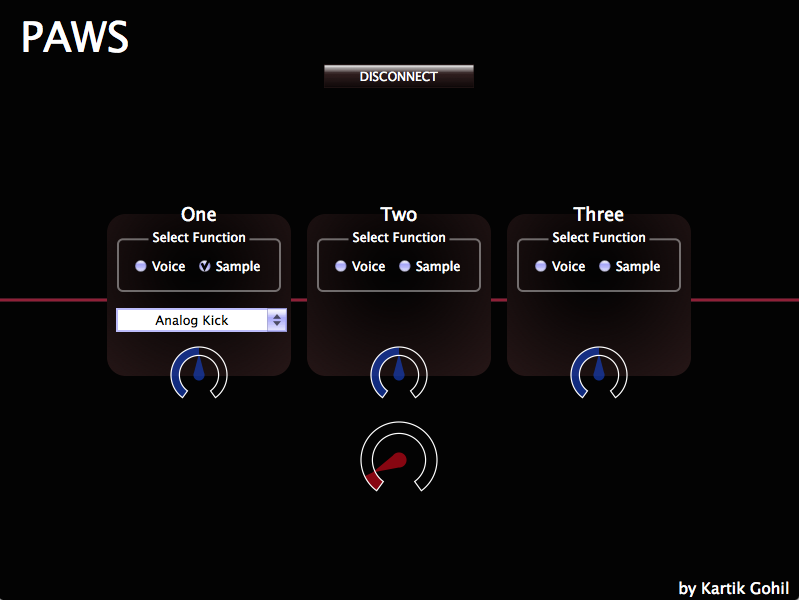
\includegraphics[scale = 0.5]{Images/paws_3_single}
\caption{Interface showing controls for 3 Finger Boards, Prototype 0.2.04}
\label{fig:paws_3boards_final}
%\end{wrapfigure}
\end{figure}

\subsubsection{Filtering the Audio Signal}

This section summarises the attempts I made to modify the frequency content of the various signals in this Prototype.

Firstly, the Arduino Shield I designed in Section~\ref{0203} Prototype 0.2.03 was made to provide analogue voltages from the Arduino to control the gains of the amplifiers on the Finger Boards. I realised that the resistor-capacitor filters for converting the Arduino's PWM (Pulse Width Modulated) signals to analogue voltages were placed on the Finger Boards instead of on the Shield. This meant that the PWM signal was being transmitted down the jack cable between the Shield and the Finger Boards, and was therefore affecting the microphone signal coming back down the cable. In order to remedy this as quickly as possible, I designed a new PCB for the Arduino Shield, which filtered the PWM signals first before sending them to their respective Finger Boards. The transmission of a constant analogue voltage down the cable would therefore not induce any noise onto the microphone signal as it would not host any high frequency content. Appendix~\ref{ardshieldpcb2} shows the PCB Layout for Version 2 of the Arduino Shield.

Since Version 2 of the Arduino Shield was not printed in time for the report, Prototype 0.2.04 continued using Version 1 and the induced PWM noise was the main source of distortion in the resultant microphone signal. 

I also attempted to implement software filtering of the microphone signal, firstly to try to reduce the effects of the PWM on the signal, and secondly to isolate the frequencies related to 'tapping' a Finger Ring against a surface for robust sample triggering. JUCE contains libraries for determining filter coefficients and applying them to a chunk of samples. In order to conform to this library's requirements, I briefly modified my Arduino's code to read and transmit an entire chunk of data (arbitrarily set to ten data samples), which the Interface would read and store into a temporary buffer and filter before adding them to the Queue as before. However, I had troubles with determining filter coefficients for the low pass filtering I wished to do with a cutoff around 500Hz to ensure that only 'tapping' energy was kept in the spectrum. In order to workaround this problem, I used Matlab to determine coefficients and then imported them into my program to implement them and hence filter the input chunk. I found that for each set of coefficients I tried (with various cut off frequencies and roll offs) my microphone signal became unstable, sometimes producing sample values of the thirty-second order. Considering that audio signals are normally defined as float-type variables within the range of -1 to 1, this instability was either a result of poorly defined coefficients, since JUCE implemented all filters as Infinite Impulse Response filters which have the ability to become unstable, or that the already small sample values were wrapping around to become incredibly large and therefore not producible by the system. 

Filtering in software was a necessary step, especially since I was upsampling the microphone signal to match the output sample rate of the program, which introduced spectral images that needed to be removed. However, I had to stop testing software filtering as I was not able to produce a stable result within a reasonable amount of time. More testing could be done using a bespoke filtering function rather than JUCE's methods. I was also only filtering a single chunk of samples at a time, which first of all were very small at only 10 samples per chunk, and I was not using correct Digital Signal Processing methods for filtering in real-time such as the Overlap-Save or Overlap-Add\textsuperscript{\cite{overlap}} methods. Further testing of software filtering would require implementing these well-documented methods to ensure stability and accuracy. 

\newpage
%%%%%%%%%%%%%%%%%%%%%%%%%%%%%%%%%%%%%%%%%%%%%
\section{Product Evaluation} \label{Evaluation}

This section aims to analyse and critique Prototype 0.2.04 both quantitatively by looking at the hardware and software, and qualitatively in how it stands up to the requirements of the Product Concept and through user testing. 


\begin{wrapfigure}[33]{r}{0.4\textheight}
\centering
\subfloat[No Finger Boards attached]{
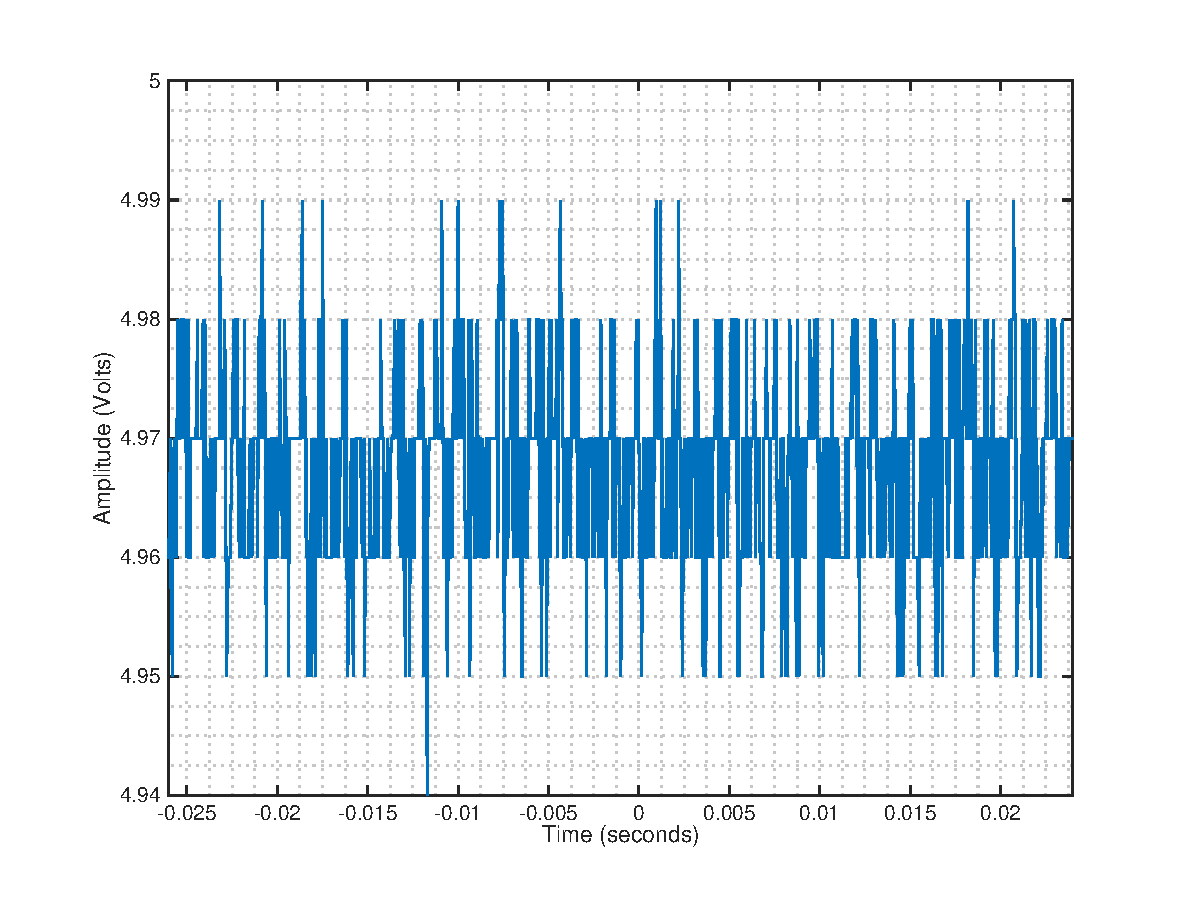
\includegraphics[width=0.4\textheight, height=0.15\textheight]{Images/rail_noboards2.eps}
\label{fig:rail_noboards}
}
\\
\subfloat[1 Finger Board attached]{
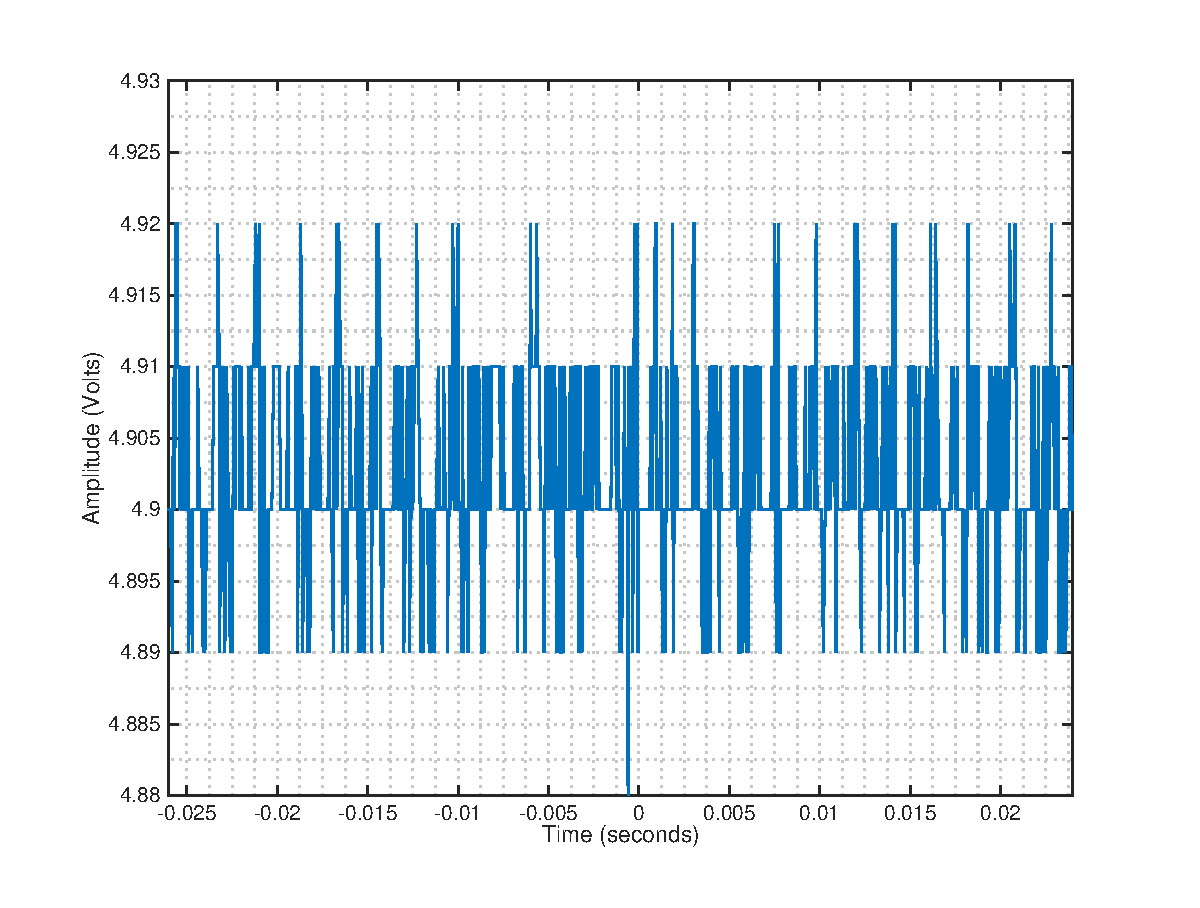
\includegraphics[width=0.4\textheight, height=0.15\textheight]{Images/rail_1board2.eps}
\label{fig:rail_1board}
}
\\
\subfloat[3 Finger Boards attached]{
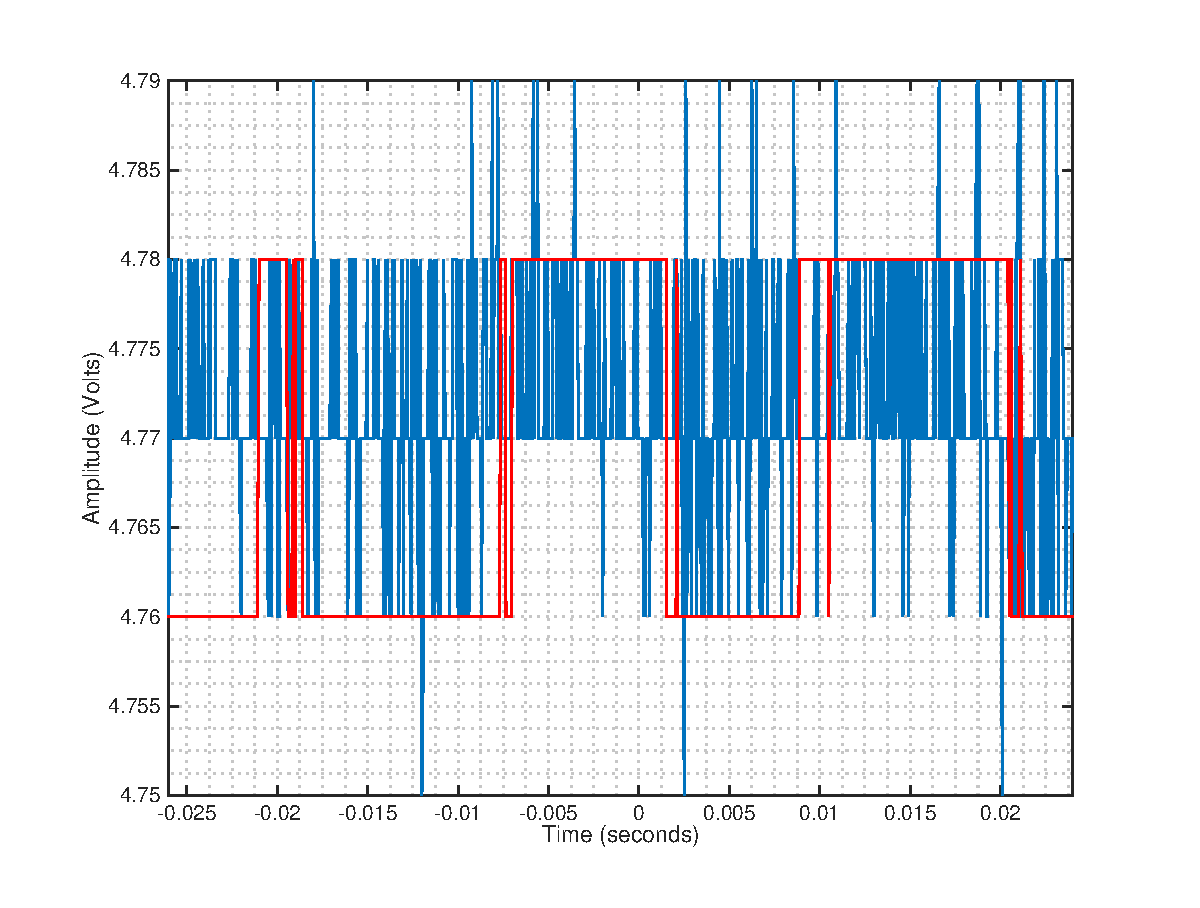
\includegraphics[width=0.4\textheight, height=0.15\textheight]{Images/rail_3boards2.eps}
\label{fig:rail_3boards}
}
\caption{Arduino 5V Power Rail measured on the Arduino Shield, connected to a different number of Finger Boards}
\end{wrapfigure}


\subsection{Prototype 0.2.04 - Analysis} \label{Prototype Evaluation}

This section quantitatively analyses particular data about the Prototype such as the effects of noise and changes in sampling rates. 

\subsubsection{Effects of Noise}

The evaluation was conducted using Finger Boards connected to Version 1 of the Arduino Shield circuit board since Version 2 was not available for testing. The tests involved looking at the noise ripple across the power rails of the Arduino and in the microphone signal coming in to the Arduino's analog input pin. All measurements were taken with a digital oscilloscope and plotted using Matlab. 

Figure~\ref{fig:rail_noboards} shows the power rail measured on the Arduino Shield with no Finger Boards connected. We can see that it is centred around 4.97V, instead of the expected 5V, and features approximately 20mV of digital noise ripple. After connecting one Finger Board to the Arduino, I found that the rail voltage dropped further to 4.9V, a drop of 70mV, with the same noise ripple of 20mV. Figure~\ref{fig:rail_1board} shows the waveform of the rail voltage for one connected Board, and Figure~\ref{fig:rail_3boards} shows the same for three. The voltage dropped significantly to 4.77V with three Boards attached but the noise ripple again remained constant at 20mV. For this Prototype, the Arduino was producing three PWM signals, all at 61Hz, for the Finger Boards to use as analogue voltages to control their programmable gain amplifiers. In Figure~\ref{fig:rail_3boards}, a red overlay has been plotted showing a low frequency periodicity in the noise ripple corresponding to the PWM signals at 61Hz. This frequency was being induced onto the power rails most likely through the jack cable attaching the Arduino Shield to the Finger Boards. 

Figure~\ref{fig:sig_1} shows the microphone signal from a Finger Board, measured at the analogue input pin on the Arduino Shield. The signal has been listed as being in an \textit{idle state}, meaning that no deliberate sounds were made; the microphone was only capturing the background noise of the labs and the electrical noise of the circuitry. The signal is centred around 2.41V as opposed to the expected 2.5V, and this is most likely due to the rail voltage not being exactly at 5V. We can see large spikes in the waveform due to the induction of the PWM signal, which I temporarily returned to its original 490Hz for graphical clarity. The frequency response plot confirms that the periodic spikes do in fact correspond to the 490Hz of the PWM signal. We can also see a high amount of energy around the 10kHz mark, most likely corresponding to thermal noise, which was previously found to be present and was temporarily dealt with using a simple low pass filter with a cut-off of 20kHz. Of course, the best solution to remove this noise would be to research further into thermally isolating the microphone and its circuitry. 

\begin{figure}[H]
\centering
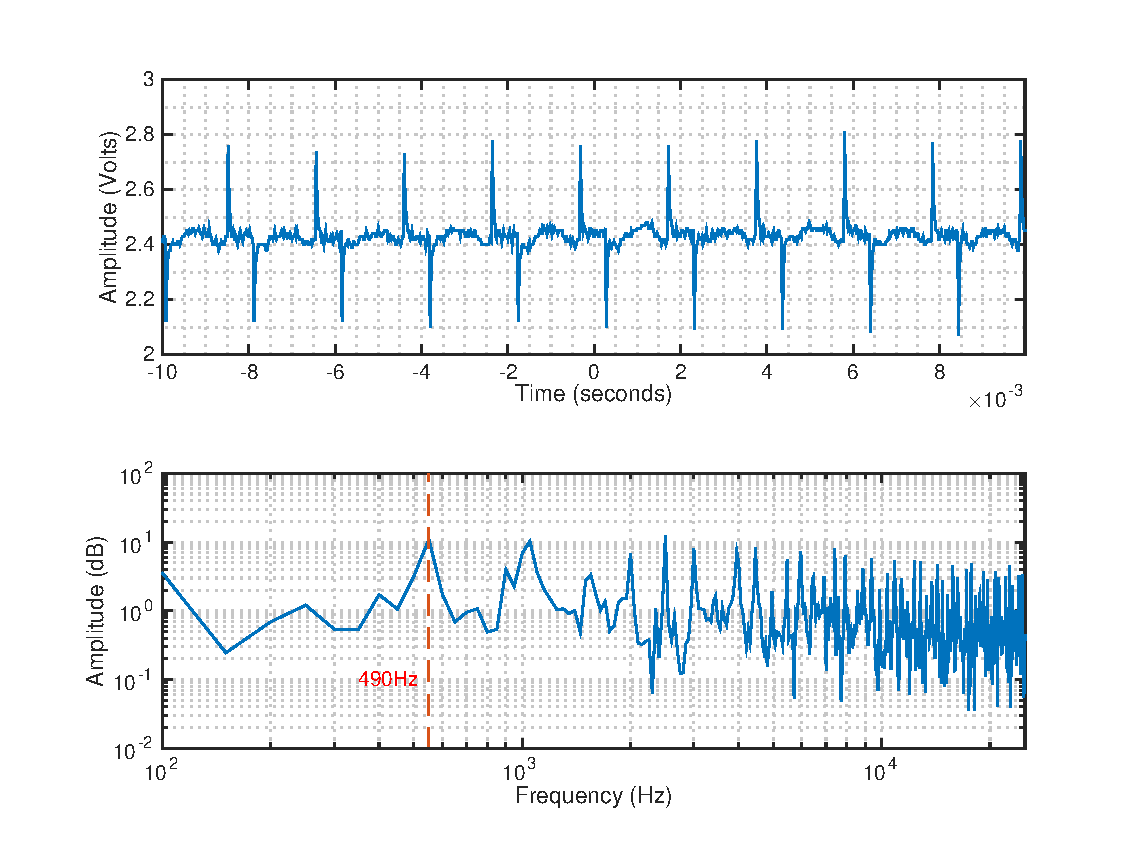
\includegraphics[width=0.55\textheight, height=0.4\textheight]{Images/sig_1.eps}
\caption{Microphone Signal (idle state) measured at the Arduino input pin, with PWM Frequency at 490Hz}
\label{fig:sig_1}
\end{figure}

\begin{wrapfigure}[24]{r}{0.37\textheight}
\centering
\subfloat[Idle State (no deliberate input)]{
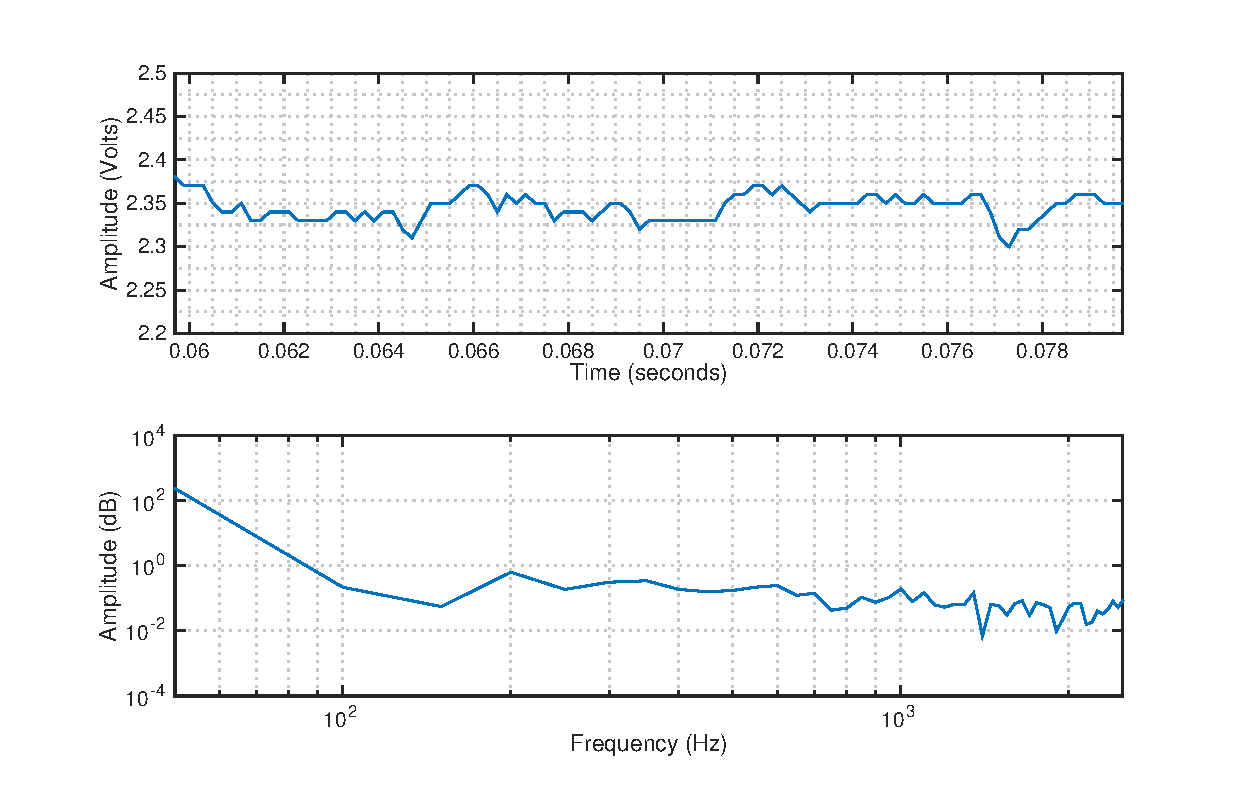
\includegraphics[width=0.4\textheight, height=0.3\textheight]{Images/sig_2_idle.eps}
\label{fig:sig_2_idle}
}
\caption{Microphone Signal measured at the Arduino input pin, with PWM Frequency at 30Hz}
\end{wrapfigure}


Figure~\ref{fig:sig_2} shows the same microphone signal but with the PWM Frequency now at 30Hz, which is the lowest frequency the Arduino was able to produce. We can see that the waveform is more stable in the idle state, Figure~\ref{fig:sig_2_idle}, and the frequency response much flatter. The noise ripple has been greatly reduced to a maximum of 100mV, as opposed to 700mV with the PWM at 490Hz. Figure~\ref{fig:sig_2_tap} shows the microphone picking up the sound of a Finger Ring, with a Board attached, tapped against a wooden table. The analogue signal is clearly visible amongst the noise ripple and we can see the increase in energy at frequencies of 600Hz and around the 1kHz mark as compared to the idle state. 30Hz is the lowest PWM frequency producible by the Arduino Uno but only for a select few of the analogue output pins. The way in which Prototype 0.2.04 has been wired limits the lower bound of the PWM frequency of the second and third Boards to 61Hz, and therefore the first Board must also be set to this value to ensure the Interface's processing code works in the same way for each of the Boards. The reason for the induced PWM signal having a smaller effect at lower frequencies could be because of the Programmable Gain Amplifier's high pass filtering at each of its input pins. I designed it such that the high pass cutoffs were at 90Hz, meaning that frequencies lower than this would be attenuated by an order of 2 (since the amplifier consisted of two gain stages). 

\begin{figure}[H]
\ContinuedFloat
\centering
\subfloat[Tapping the Finger Ring against a table]{
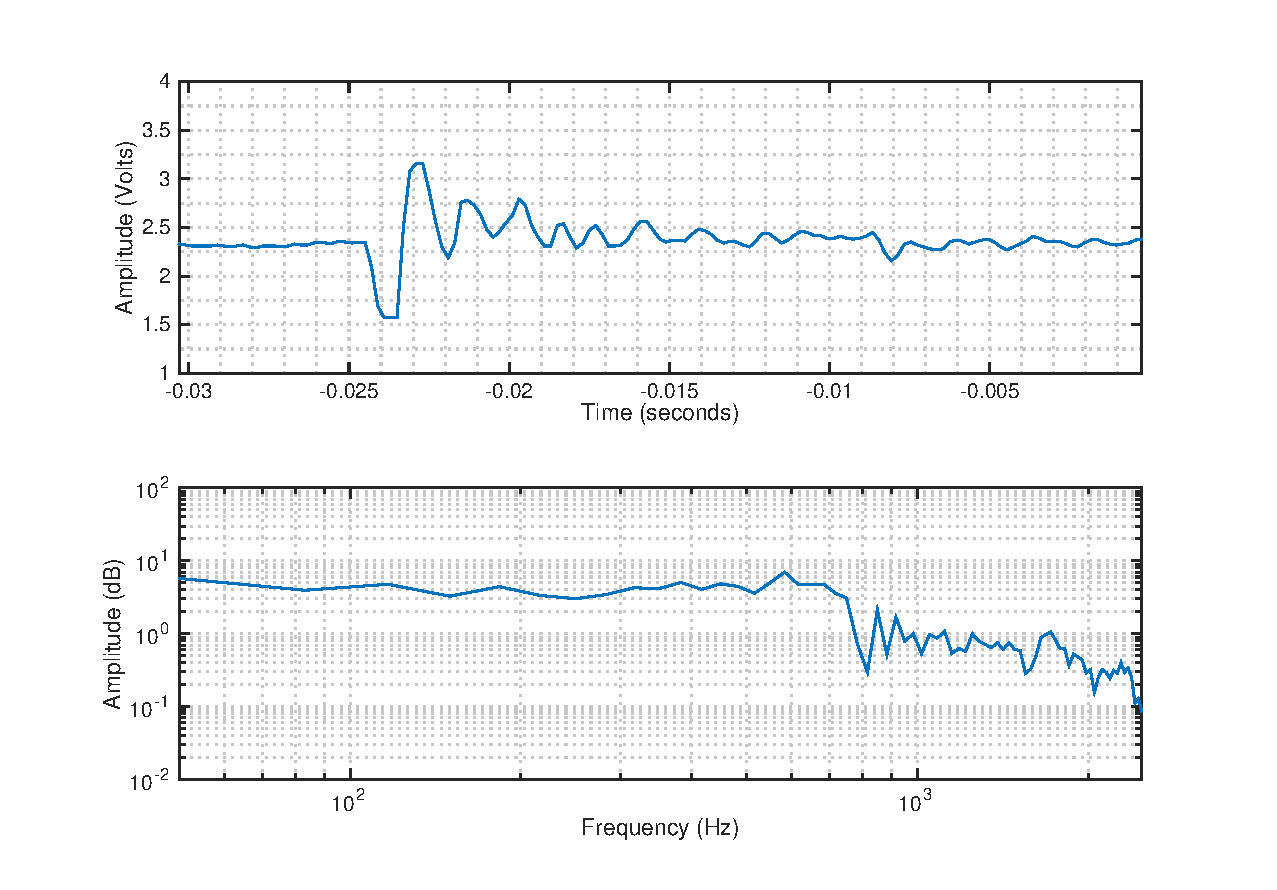
\includegraphics[width=0.4\textheight, height=0.3\textheight]{Images/sig_2_tap.eps}
\label{fig:sig_2_tap}
}
\caption{Microphone Signal measured at the Arduino input pin, with PWM Frequency at 30Hz}
\label{fig:sig_2}
\end{figure}

\subsubsection{Sample Rates}

The Arduino Uno was responsible for sampling the microphone signals of all connected Finger Boards and transmitting them to the Interface. According to Arduino's documentation, the \textit{analogRead(~)} function responsible for sampling input voltages is limited to generating 10,000 samples per second\textsuperscript{\cite{analogread}}. However, since the code samples each connected Finger Board and transmits them in turn, along with a single new line character used as a 'start of packet' indicator at the very beginning, the effective sample rate is considerably hampered. This change in sample rate affects both the frequency content of the signal able to be captured and the upsampling ratio needed to produce a signal at a sample rate of 44.1kHz to be outputted by the Interface to the audio device. 

I changed the packet size (i.e. the number of Finger Boards I sampled and transmitted in each loop) and then calculated the time taken to process the entire packet, including both sampling and transmission. This processing time can be argued to be the sample period of a signal, since this is the time taken before another sample can be taken for a particular signal. Therefore, the sample rate of each signal $f_s = \frac{1}{time/packet}$. From this I was able to calculate the effective sample rate, or the overall number of samples read per second by the Arduino, with the equation $f'_s = \frac{samples/packet}{time/packet}$. This effective sample rate gives us an idea of the fraction of time we spend per packet on sampling data as opposed to transmitting data, and can be compared against the Arduino's rated frequency of 10kHz. From the signal sample rate $f_s$ we can also determine the upsampling ratio required by the Interface to transform the signal to its required rate of 44.1kHz. The upsampling ratio is calculated as $ratio = \frac{44.1}{f_s}$ and these values are shown in Table~\ref{tab:packeteval}.

\begin{table}[H]
\begin{center}
\begin{tabular}{r| l l l l}
Samples  & Processing Time & Signal Sample & Effective Sample  & Upsampling  \\
per Packet  & per Packet (ms) & Rate (ksamp/sec)   & Rate (ksamp/sec)    & Ratio \\ \hline
1   &   0.17    &   5.882   &   5.882   &   7.50 \\
2   &   0.281   &   3.559   &   7.117   &   12.39 \\
3   &   0.42    &   2.381   &   7.143   &   18.52 \\
\end{tabular}
\end{center}
\caption{Table showing sample rates for different data 'packet' sizes}
\label{tab:packeteval}
\end{table}

We can see that even though it takes longer to process larger packets, the effective sample rate seems to increase. This is due to the fact that with a packet size of one sample, half of the transmitted packet is the starting 'new line' character, and the second half is an actual sample value, whereas with a packet size of 3, the 'new line' character only takes up a quarter of the packet and the packet contains 3 sample values. This means that because less processing time is being spent towards transmitting the 'new line' character relative to sampling, we are able to produce more samples per second, which directly corresponds to an increase in sample rate. 

%\begin{figure}[H]
\begin{wrapfigure}[22]{r}{0.37\textheight}
\centering
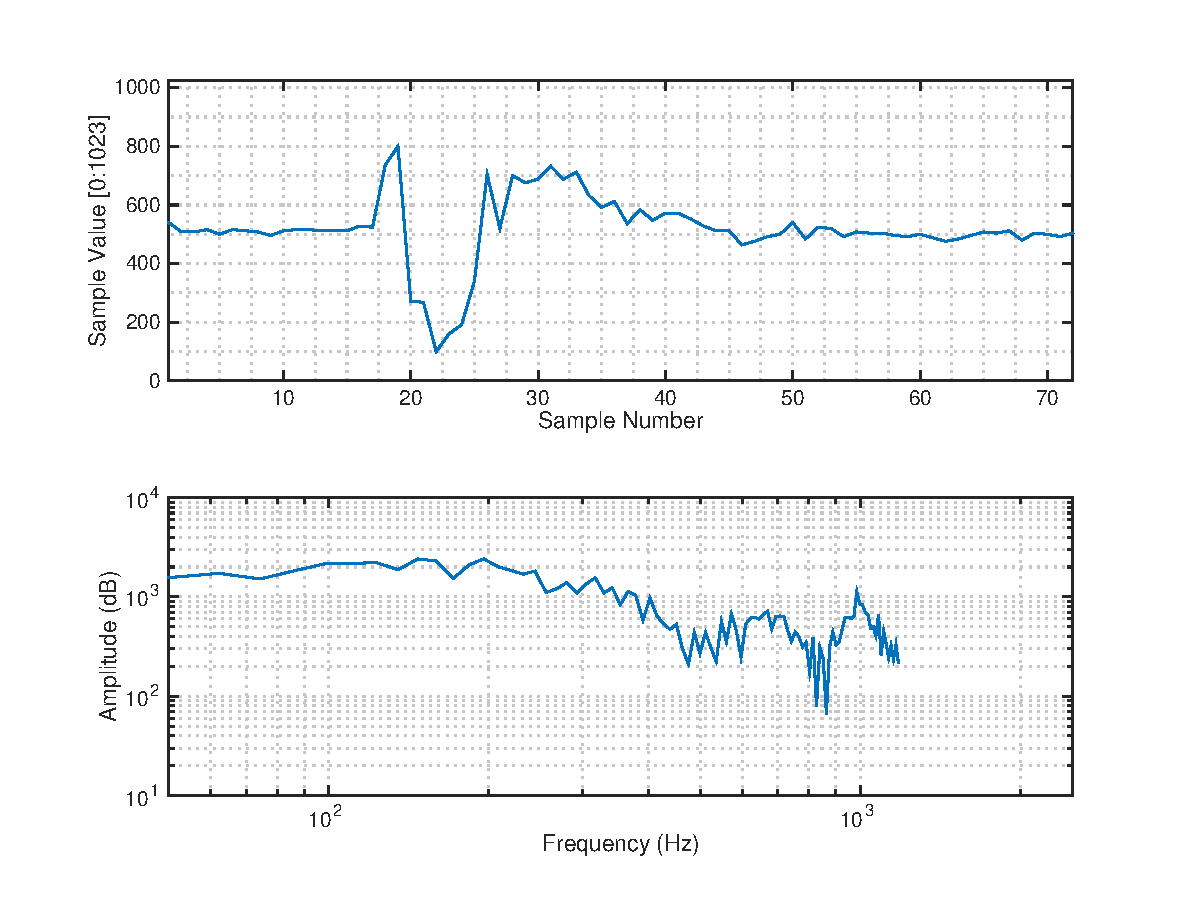
\includegraphics[width=0.4\textheight, height=0.3\textheight]{Images/sig_samp.eps}
\caption{Microphone Signal sampled at 2.381kHz, received by the Interface program}
\label{fig:sig_samp}
\end{wrapfigure}
%\end{figure}

We can also see that the signal sample rates are very low, even worse than a telephone line, which is usually sampled at 16kHz. This means that the intelligibility of any voice information captured will be almost non-present, however, the signal will still be able to pick up 'tapping' sounds, which seem to feature high energies at 600Hz and 1kHz, according to Figure~\ref{fig:sig_2_tap}. The calculated upsampling ratios directly correspond to the values I used in Prototype 0.2.02, detailed in Section~\ref{0202}, which I settled upon simply through trial and error and matching the frequency of my voice with what was being played back through the Interface in 'Voice' mode. 

Figure~\ref{fig:sig_samp} shows a microphone signal capturing the 'tap' of a Finger Ring against a workbench as data samples received by the \textit{queueInput(~)} function of the Interface. We can compare this signal against the continuous-time one in Figure~\ref{fig:sig_2_tap} which was measured at the Arduino's input analogue pin. The discrete-time signal does indeed have a similar waveform but, as we can see, its frequency response is capped due to the previously calculated sampling rate of 2.381kHz. This low sampling rate also causes distortion to the signal's waveform through loss of temporal precision and accuracy. 



\begin{wrapfigure}[14]{r}{0.37\textheight}
\centering
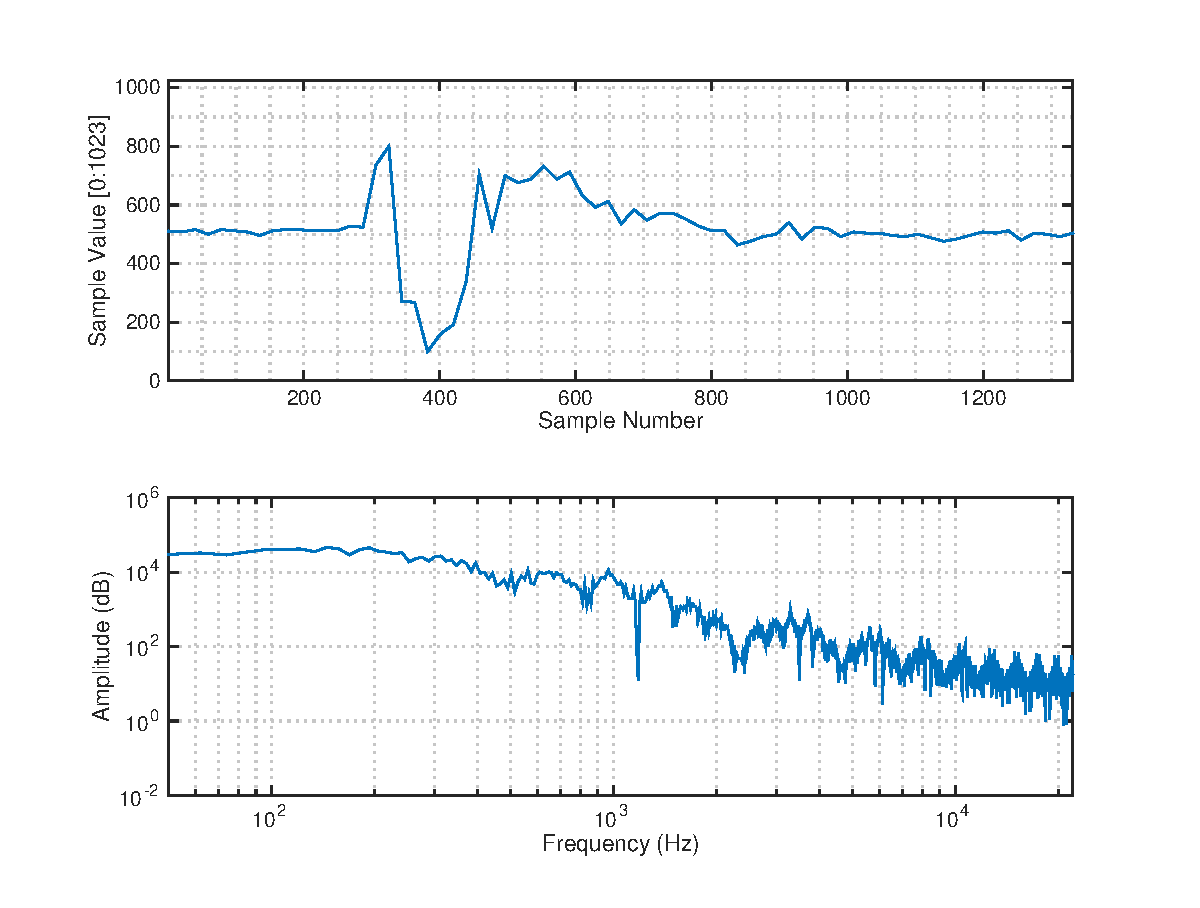
\includegraphics[width=0.4\textheight, height=0.3\textheight]{Images/sig_oversamp.eps}
\caption{Microphone Signal upsampled to 44.1kHz, played by the Interface program}
\label{fig:sig_oversamp}
\end{wrapfigure}

Upsampling of the signal in the 'Voice' function to 44.1kHz introduces spectral images, which will cause distortion since the original signal is bandlimited to only 1.191kHz, and the frequency response will be duplicated every 2.381kHz up to the audible range limit. These spectral images can be seen clearly in Figure~\ref{fig:sig_oversamp}. The linear interplation method used to upsample maintains the signal's time-domain waveform but all of the images in the spectrum are audible, and therefore act as noise. The signal would be required to be filtered post-upsampling so as to remove these artefacts.



\newpage
\subsection{Prototype 0.2.04 - Evaluation} \label{Prototype Evaluation 2}

This section qualitatively evaluates the Prototype by comparing it against the Product Requirements and through User Testing.

\subsubsection{Requirements Evaluation}

Prototype 0.2.04 was evaluated against the specifications detailed in Section~\ref{Requirements} Product Requirements to determine which areas of the Concept Design were implemented and to highlight the areas where further development was necessary. 

Table~\ref{tab:specifications} listed specifications for both a concept PAWS Board and the Interface. Table~\ref{tab:specificationsmet} answers these specification questions to determine what the Finger Board, coupled with the Arduino, and the JUCE Interface for Prototype 0.2.04 can and cannot do. 

\begin{table}[H]
\centering
\begin{tabular}{|l}
\textit{The PAWS Board (Finger Board + Arduino)}\\ \hline \hline
It can capture audio. \\
It can modify the amplitude of the audio signal.\\
It can connect to the Interface \\
It can send captured data to the Interface via wired transmission\\
It is wearable through 3D printed attachments\\
\hline
It cannot modify the frequency content of the audio signal\\
It cannot capture motion \\
It cannot send captured data to the Interface via wireless transmission\\
It is not very comfortable to wear\\
It cannot be switched on and off\\
It cannot remind the user of its functionality\\
It cannot be carried in a pocket or bag\\
\hline  \hline 
\textit{The Interface} \\ \hline \hline
The Interface is available on a computer \\
It can connect to PAWS Boards \\
It can read data sent by the connected PAWS Boards\\
The user can control the function of every connected PAWS Board \\
It can modify the amplitude of the audio signal from each PAWS Board\\
It can open and play sample sound files\\
It can trigger sample sound files from PAWS Board data\\
It can output the generated audio to the output audio device \\
\hline
The Interface is not available on a smartphone \\
It cannot save the output audio to file\\
It cannot modify the frequency content of the audio signal from each PAWS Board\\
It cannot map motion gestures to control parameters\\
\end{tabular}
\caption{List of Specifications met by Prototype 0.2.04}
\label{tab:specificationsmet}
\end{table}

We can see that the Finger Board and Arduino have not been developed to the same extent that the Interface has, particularly because adding new functionalities in hardware requires much more time and effort than with software. A few of the specifications have been answered vaguely, for instance, the Finger Board does perform low pass filtering on the microphone signal but since the question is asking whether the filtering of the signal can be freely programmed, it has been listed in the 'cannot do' section. Similarly, the question '\textit{Can it remind the user of its functionality?}' is open and would probably require further details into how it would do that once a method to do so has been implemented. 


Table~\ref{tab:criteria} from Section~\ref{Requirements} listed a few open-ended questions in an aim to incite a discussion on a Prototype's functionality as opposed to marking off a checklist. Table~\ref{tab:criteriamet} provides a summary of how Prototype 0.2.04 has met these criteria. 

\begin{table}[H]
\centering
\begin{tabular}{|l}

\textit{Functionality} - What can the instrument do?\\
\hline
The instrument can capture audio using a microphone and either feed it through the computer's audio\\ 
output using the 'Voice' function or trigger sample sound files in response to user 'taps' using the 
\\'Sample' function.\\
\hline \hline
\textit{Portability} - How easy is the instrument to carry?\\
\hline 

The Finger Boards can be worn very easily on fingers but the attached Arduino must be close to a \\
computer and therefore the entire instrument is not very portable.\\

\hline \hline
\textit{Setup Time} - How long does it take to ready the instrument?\\
\hline 

It takes approximately a minute to ready the instrument: the Finger Boards must be connected to\\ 
the Arduino with the correct cables, the Arduino must be connected to the computer with a USB \\
cable, and the Interface must be loaded (which can currently only be run in debugging mode through\\
the Development Software \textit{Xcode}; it is not available as a standalone application). The Arduino must\\
also be connected to a particular USB port on my computer in order to be detected by the program. \\

\hline \hline
\textit{Performance} - Does it do what it has been programmed to do? \\
\hline 

The instrument does exactly what it has been programmed to do. This is due to the fact that Prototype \\
0.2.04 was streamlined to be demonstrable with the current setup of a single Arduino and 3 Finger \\
Boards, and therefore all non-implemented functionalities were removed. \\

\hline \hline
\textit{Flexibility Of Use} - What can the user do with the instrument?\\
\hline 

The user can speak into the Finger Board's microphone using the 'Voice' function but cannot hear \\
themselves very well due to the low sampling rates and digital noise affecting the resultant signal. \\
The user can also play three different sample sound files using the 'Sample' function, but the files \\
they can play are limited to the few that have been made available. \\
They currently do not have the ability to add their own files. \\

\hline \hline
\textit{Simplicity Of Use} - How easily can the user program PAWS Boards? \\
\hline

The programmability of the Interface is incredibly simple. The user only has to select which mode \\
they require, 'Voice' or 'Sample', and the program will automatically do what is required of it. If the \\
'Sample' function is selected, the Interface will display a drop down list for the user to choose which \\
sample sound file gets triggered. This selection has been implemented deliberately as a drop down \\list to allow for the user to add as many sample sound files as they wish. Volume pots are available to \\
change the amplitudes of the signals from each of the Boards individually as well as a global \\volume control.\\


\hline \hline
\textit{Spatial Limitations} - Is the instrument physically restrictive in its use?\\
\hline
The prototype is in fact extremely restrictive. The Finger Boards, along with the Rings, are large and \\heavy, and the cables attaching them to the Arduino are thick and somewhat impair the user's ability \\to move their hand freely. The user must also remain close to the computer running the Interface \\program since the Arduino is connected to it via a USB cable and must sit comfortably on a surface. 

\end{tabular}
\caption{Discussion of Criteria met by Prototype 0.2.04}
\label{tab:criteriamet}
\end{table}


\newpage
\subsubsection{User Testing} \label{User Testing}

%\begin{figure}[H]
\begin{wrapfigure}{r}{0.4\textheight}
   \centering
   \includegraphics[scale=0.14]{Images/paws_testrig2} 
   \caption{Prototype 0.2.04 Finger Boards arranged on workbench for User Testing}
   \label{fig:testrig}
\end{wrapfigure}
%\end{figure}

After performing the Requirements Analysis myself, I sought to find a non-musician as a potential user to test my Prototype. Considering that the 'Sample' mode for Prototype 0.2.04 worked to the extent where samples could be triggered by physically tapping the microphone but not through the detection of the Finger Rings impacting upon a surface, I decided to secure my Finger Boards to a workbench for my user to interact with and still be able to test the functionality of my instrument. Figure~\ref{fig:testrig} shows a still frame from video footage of the user testing session, and simultaneously shows the the PAWS Interface and the user's interaction with the Boards, which have been held down in a row using electrical tape. 



For the purposes of anonymity, I will hereby refer to the user who tested Prototype 0.2.04 as 'The User'.

I began the test session by asking The User some preliminary questions. The User claimed to have to prior experience with musical instruments and, when asked why, claimed to not have any particular interest and had always been put off by the amount of time that would have to be set aside to learn and practice.

I then gave The User a quick overview of the Interface program and observed how they interacted with it. The User immediately began to switch the Boards into 'Sample' mode and selected random sound files for playback. Since I had laid out the Finger Boards on the table in the order they were connected to the Arduino, it was easy for The User to map the controls on the Interface to the correct Boards. The User tapped the microphones and produced a rhythm very quickly. The User claimed that the Interface was intuitive and produced the expected responses, such as the dynamic volume control and visual feedback of the audio signal. 

After letting The User spend some time with the instrument, I asked a few follow up questions. I firstly asked what The User was able to do with the instrument and they said that they spent the entire time in 'Sample' mode playing with the various sound files. When asked what they would like to be able to do with the instrument, The User said that they would like the feature to record custom sound files and add them to the list of available files. I suggested that the 'Voice' mode could be modified to be able to record captured audio and the recorded file could be used in 'Sample' mode, thus giving a user further freedom for creativity. 

Finally, I asked The User what features of the instrument they did not like. The first thing that was mentioned was its portability. I let The User wear the Finger Boards with the Rings to allow them to test what it would be like to tap a rhythm against the workbench as conceptualised. The User mentioned that the Rings were uncomfortable; the lip dug into their skin and the long Board restricted the range of motion of their fingers. They instinctively wore the Boards with the jack cables leading away from their fingertip as opposed to the intended way of leading down the back of their hand, and they found that the jack cables weighed their fingers down and reduced their mobility. I mentioned the concept design for wireless PAWS Boards much smaller than the current Finger Boards and The User agreed that that would solve the mobility issue. 

The User provided additional ideas for potential improvements, such as designing the Interface so that it reflected the look and feel of the hardware Finger Boards to create a stronger connection between the two. The User also requested wearable housings other than Rings, such as bands to be worn around the wrist or palm. The User was very interested in the future scope of the instrument, and the ability to use it for more than just music, such as a remote for controlling other applications, or even to control elements of the PAWS Interface through dedicated gestures such as clapping two Boards together. 

All in all, The User found the PAWS instrument very accessible as a non-musician, in that it would allow for people with a vast range of experiences to easily create music, and if correctly made portable, would allow for use on the go, thereby reducing the time limitations with learning how to play traditional instruments. 



\newpage
%%%%%%%%%%%%%%%%%%%%%%%%%%%%%%%%%%%%%%%%%%%%%
\section{Project Evaluation} \label{Progress Evaluation}

This section aims to evaluate the progress of the entire project against initial expectations. Table~\ref{tab:listofprototypes} from Section~\ref{Implementation Plan} Implementation Plan shows a list detailing a plan of the successive development of prototypes. Table~\ref{tab:listofprogress} shows the actual progress I made over the duration of the project as a list of prototypes and their key features. 

The actual progress varied quite significantly from the projected plan, mainly due to the initial Python program not being able to handle audio processing code quickly enough. As discussed in Section~\ref{0201}, Prototype 0.2.xx involved a changeover to the JUCE library in C++, for which I had to completely restructure my program and re-implement everything I had done in Python. I also spent more time on making the GUI more engaging with an end-user oriented design and modern visuals. I was able to implement the Programmable Gain Amplifier (PGA), as planned, but it was mostly used for its cleaner signal over the Operational Amplifier circuit rather than its gain control capabilities. Printed Circuit Boards and 3D Printed wearable Rings were also produced later on, as wished for in the plan. 

\begin{table}[H]
\begin{center}
\begin{tabular}{|l l}
Prototype  &   Features \\ \hline \hline
0.1.01 &    Basic microphone circuit and test 'Voice' and 'Sample' functions in Python\\
0.1.02 &    Full Python Program with GUI to control 'Voice' and 'Sample' modes \\
0.1.03 &    PGA in circuit for digital gain control   \\ \hline
0.2.01 &    New Program Structure and GUI designed using JUCE for C++ \\
0.2.02 &    Implementation and Optimisation of 'Voice' and 'Sample' functions and data transmission  \\
0.2.03 &    All hardware on PCBs and 3D printed wearable housings \\
0.2.04 &    Modification of Program to connect to multiple Boards simultaneously    \\
\end{tabular}
\end{center}
\caption{Actual Implementation Progress as a List of Prototypes and their Features}
\label{tab:listofprogress}
\end{table}

Much of my project was dedicated to optimising audio processing code: in the sampling stage at the Arduino, the transmission between it and the computer, and all of the processing and data handling within the Interface itself. The algorithms to upsample the input signals and to trigger sample sound files took the most time to code and improve, in order to ensure robustness and accuracy. The User Interface was focused upon with great detail too to ensure easy usability and an appealing look.

\begin{wraptable}[19]{r}{0.3\textheight}
\begin{center}
\begin{tabular}{| l r r}
Prototype   &  Start Date &  Completion \\
& (2015) & Date (2015)\\ \hline
0.1.01  & - & 20 Jan \\ \hline
\hline \emph{Interim Report} & -&2 Feb \\ \hline \hline
0.1.02  & 2 Feb &20 Feb\\ 
0.1.03  &  20 Feb		&14 Mar\\  \hline
0.2.01  & 	14 Mar	&19 Mar\\
0.2.02  & 	22 Mar	&14 May\\
0.2.03  & 	20 Mar	&8 Jun\\ \hline
\hline \emph{Abstract} & 1 Jun &8 Jun \\ \hline \hline
0.2.04  & 	25 May	&12 Jun\\ \hline
\hline \emph{Final Report} & 5 May & 17 Jun \\ \hline
\hline \emph{Presentation} & - &24 Jun \\ \hline
\end{tabular}
\end{center}
\caption{Actual Implementation Progress as a Timetable of Deliverables}
\label{tab:progressplan}
\end{wraptable}

Table~\ref{tab:progressplan} shows how long it took to implement each of the prototypes, in order of their completion dates. These dates have been pulled from my project logbook and we can see that work for the earlier prototypes was linear whereas later work was done almost simultaneously. For example, I began designing the PCBs for Prototype 0.2.03 near the end of March, even before work on 0.2.02 properly began, but I did not finish printing the final batch of 3D printed Rings until 8th June. There was a large gap in implementation between the end of March and the end of May due to exams but I continued to make small amounts of progress in different areas, sometimes working on 3D sketches for the Finger Rings, ensuring that my PCBs were printed and soldered, and I even began typing up the report early on. 

The aim of this project was to implement a version of the conceptualised PAWS instrument that could demonstrate the 'Voice' and 'Sample' modes and the instrument's flexibility of use. Prototype 0.2.04 was created to demonstrate the programming of multiple Boards independently of each other, despite it being far from the original requirements of being portable and giving the user freedom of musical expression. However, I believe that this Prototype has shown great scope for further development and forms a good starting point as a proof-of-concept of the PAWS concept. 

\newpage
%%%%%%%%%%%%%%%%%%%%%%%%%%%%%%%%%%%%%%%%%%%%%
\section{Improvements \& Enhancements} \label{Further Developments}

\subsection{Future Design, Prototype 0.3.xx} \label{03xx}
\subsubsection{The PAWS Board}
Prototype 0.2.04 was fairly bulky in design relative to the concept design and any further developments would need to remedy this. I realised that the only need for the Arduino Uno was to sample the connected microphone signals and transmit the captured data to the Interface where all of the processing was done. It was of course also used to set the gain of the microphone circuits' amplifiers but this function was not used in the initially intended way and in fact the gain was kept constant during run-time. 

Therefore, the Arduino Uno could be deemed to be a redundant component for what it was used to do, and could simply be replaced by an Analogue-to-Digital Converter (ADC) and a Serial interface. This would mean that the entire circuitry could be contained on a single Finger Board, which would connect directly to a computer. A good enough ADC would also be able to detect the microphone signal's dynamic range and map the incoming voltages to the entire digital range of values, thereby removing the need for a bespoke amplifier. Some surrounding digital circuitry may also be required, such as a clock, and Figure~\ref{fig:0304_circuit} shows a mock-up system design for the Finger Board.

\begin{figure}[H]
\centering
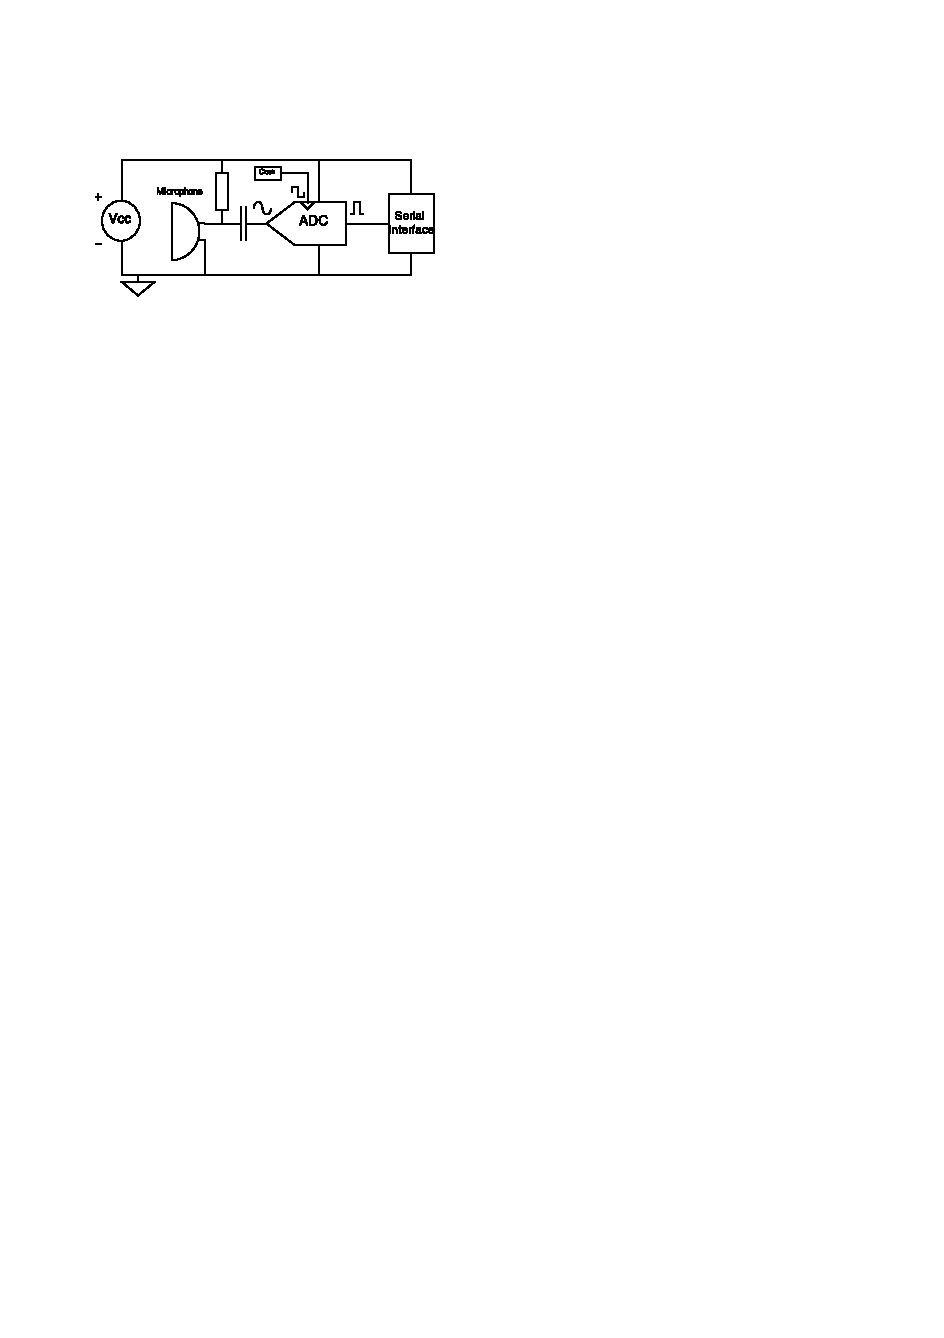
\includegraphics[scale=2]{Images/FutureDesign}
\caption{High-Level System Design for a PAWS Board, Prototype 0.3.xx}
\label{fig:0304_circuit}
\end{figure}

The inclusion of a battery would clean up the rail noise significantly compared to drawing power from the computer and suffering additive noise from the Arduino. The Serial interface could be a simple Micro-USB connector or even a Bluetooth transmitter. The microphone could also be thermally isolated to remove all thermal noise from the signal path, which is currently only being low pass filtered and therefore remains present in the audio frequency. Ground planing of the PCBs, where the components on the board are surrounded by a layer of silicon at ground potential,  would also aim to reduce reactive noise in the signal path. 

Other improvements could involve oversampling methods, where a signal is sampled at a much higher frequency than required, to allow for better definition and robustness to transmission errors. The coding of data for transmission could also be looked into further to increase the transmission rate by first analysing the sent signals in terms of entropy and defining smaller codewords to be sent between the PAWS Boards and the Interface. In this case, a trade-off would have to be found between oversampling, which corresponds to more data per second, and coding, which aims for less data per second. 

\subsubsection{The Interface}

As found in Section~\ref{User Testing} User Testing, the Interface would have to be modified to visually display a representation of the physical PAWS Boards to enhance the connection between the two. Prototype 0.2.04 displays controls that are intuitive to use but are not visually related to the actual hardware. Therefore, the Interface needs to be vastly improved to form a true visual counterpart to the PAWS instrument. Research can also be conducted into design methods for implementing interactive visuals, such as through Skeuomorphism, Flat Design, or Material Design\textsuperscript{\cite{materialdesign}}. 

The Interface would also require better processing of incoming audio data. Filtering the audio signal, as described in Section~\ref{0204} Prototype 0.2.04, is a major responsibility of the program. The data transfer between the PAWS Board and the Interface would have to be such that a large chunk of data samples (say 512 samples) could be received, filtered using standard digital signal processing methods, and then temporarily stored for future recall. Precise control over the reading and writing of sample data from and to buffers would be needed to ensure that data samples were not lost or missed, especially with circular buffers. 

\subsection{Further Creative Functionalities}

Further Prototypes would require additional functionality based on motion gestures, as described in Section~\ref{Concept Design} Product Design. 

The embedding of accelerometers would vastly increase the functional range of the instrument. Accelerometers are able to detect acceleration, and so they could be used to map movements or motion gestures to perform tasks. First of all, accelerometers may be better suited to the implementation of the 'Sample' mode as they would be able to detect the sudden change in acceleration when colliding with a surface. This may turn out to be a more robust solution than looking at an audio signal from a microphone, however there still remains the ability to be mis-triggered through random human motions.

There are a vast number of things accelerometers could be programmed to do. They could allow the user to pretend to strum a guitar, in response to which the Interface would play back guitar chords, or synthesise tones with pitch and amplitude data set by macro-motions (e.g. whole-arm movements) and details such as vibrato or modulation set by micro-motions (e.g finger movements). There is a great scope for how accelerometers could enable a user to be creative with their music production, which is currently very limited with microphones. 

Some functionalities to increase user feedback would probably be much appreciated. For example, a 'Blink' function could be added whereby the user could tell a particular PAWS Board to 'Blink' or identify itself through the Interface, and the Board would host an LED or some such device to respond to the command. Thus, the user would be able to quickly and easily map the physical location of a PAWS Board to its respective controls on the Interface. 

Table~\ref{tab:enhancements} shows a list of all possible enhancements to give the user freedom of expression and musical creation. 

\begin{table}[H]
   \centering
   \begin{tabular}{| l l} 
   	Enhancement & Key Feature \\ \hline \hline
	Wireless Boards & Removal of wires increases mobility \\
	Small Boards & Portable and does not physically limit user \\
	Rubber Housings & Comfortable to wear and one-size-fits-all compared to plastic\\
	PAWprintS & Foldable case that arranges Boards in piano-style layout for non-worn use\\
	On-Board Controls & On/Off switches or Mode Selection done directly from Board\\
	Variety of Housings & Wristbands, Clips, etc. \\
	\hline
	Blink & Request a PAWS Board to identify itself\\
	Motion Synthesis & Synthesise tones through motion gestures\\
	Motion Control & Change parameters for other PAWS Boards through motion gestures\\
	Record & Save audio output to file \\
	Add Samples & Open and edit custom sample sound files for 'Sample' mode\\
	Quantisation & Set tempo to quantise audio signals of other PAWS Boards \\
	Harmonisation & Trigger sample at same pitch/frequency as signal from another PAWS Board\\
	Process & Modify signal of a PAWS Board using functions such as EQ, Modulation, etc.\\
	Share & Upload recorded content to a social network\\
	Presets & Save setup of PAWS Boards for instant recall \\
	MIDI & Save signal from PAWS Board as MIDI for future sample file assignment\\
	Remote & Use PAWS Boards to control Interface, e.g. switch modes\\
	Remote 2 & Use PAWS Boards to control other applications on smartphone/computer\\
	Groups & Display and control large number of Boards and show individual controls on request\\	
   \end{tabular}
   \caption{List of possible enhancements for future development of PAWS instrument}
   \label{tab:enhancements}
\end{table}

Using the complete list of enhancements, Figure~\ref{fig:pawprints} shows a concept design for future PAWS Boards and counterpart Interface. The PAW Prints (stylistically PAWprintS) idea stems from the fact that Prototype 0.2.04 could only be used in 'Sample' mode by placing the Finger Boards on a surface and physically hitting the microphones. This could in fact be transformed into a concept design using a foldable layout that held PAWS Boards side by side to be played by striking them as you would a drum. This would in fact provide a different way of using the instrument without having to wear the PAWS Boards, and the Interface could provide a matching visual display of the PAW Prints layout to provide a better connection between the software and hardware as discussed previously. 

\begin{figure}[H]
   \centering
%   \includegraphics[scale=0.5]{Images/}
   \caption{Concept Sketch of PAW Prints Interface and layout for PAWS Boards}
   \label{fig:pawprints}
\end{figure}

With a large group of PAWS Boards, the controls for each individual Board could be displayed through selecting that Board, and a 'Blink' function could even be integrated by highlighting a particular Board to ensure that it was placed in the correct location on the layout respective to the Interface. 



{\color{red} /////PAWS Prints hardware + Matching layout on Interface\\
highlighting Board shows controls\\
}

\subsection{Marketability}

All of the enhancements detailed in the previous Subsection serve to improve the user experience and how they use the instrument to produce any sound they wish. Developing these functionalities would of course take time, considering that during the scope of this project I was only able to demonstrate a fairly limited implementation, but would in fact make the PAWS instrument highly marketable. 

If a user, musician or not, was able to immediately grasp how to use the Interface to control light and portable PAWS Boards, they would be able to make music anywhere and at anytime. The fact that the concept is designed to have no or very little physical and mental restrictions is a major selling point and would in fact secure the PAWS instrument a space in the market. 



\newpage 
%%%%%%%%%%%%%%%%%%%%%%%%%%%%%%%%%%%%%%%%%%%%%
\section{Finances} \label{Finances}

This section discusses the costs of developing Prototype 0.2.04 and the expected costs of the high-level design of Prototype 0.3.xx as described in Section~\ref{03xx}. 

Table~\ref{tab:costs0204} shows a breakdown of the costs of the components used to build the three Finger Boards and the Arduino Shield. The cost of the Arduino Uno itself and the cost to print the PCBs and Finger Rings have not been taken into account. 

\begin{table}[H]
\begin{center}

\subfloat[Prototype 0.2.04]{
\begin{tabular}{|l c| r}
\multicolumn{3}{|l}{\textit{Finger Board}} \\
 \hline
Component   &   Qty.    &   Cost (\pounds) \\ \hline
   4-way Jack Cable  &   1   &   11.990 \\
   Kingstate Microphone &   1   &   1.120 \\
   AD605BRZ Amplifier   &   1   &   13.910 \\
   Lumberg 1503 4-way Jack Socket    &   1   &  0.561 \\
   Resistor MELF0204 2.2k$\Omega$   &   1   & 0.016 \\
   Resistor MELF0204 10k$\Omega$   &   2   & 0.418 \\
   Resistor MELF0204 68k$\Omega$   &   1   & 0.018 \\
   Resistor MELF0204 82k$\Omega$   &   1   & 0.258 \\
   Capacitor C3216 10$\mu$F &   7   &   0.255\\
   Capacitor C3216 100pF &   1   &   0.020\\
\hline \hline
\multicolumn{3}{|l}{\textit{Arduino Shield}} \\ \hline
Component   &   Qty.    &   Cost (\pounds) \\ \hline
    20-way 2.54mm pitch PCB Header  &   2   &   27.580 \\
    Lumberg 1503 4-way Jack Socket    &   3   &  1.683 \\
    USB Cable A/B   &   1   &   1.860 \\
    Resistor MELF0204 68k$\Omega$   &   3   & 0.053 \\
    Capacitor C3216 10$\mu$F &   3   &   0.109\\
\hline \hline
\multicolumn{2}{r|}{Cost of 1 Finger Board}    & \pounds28.565\\
\multicolumn{2}{r|}{Cost of 3 Finger Boards}    & \pounds85.700\\
\multicolumn{2}{r|}{Cost of 1 Arduino Shield}    & \pounds31.286\\ \cline{3-3}
\multicolumn{2}{r|}{Total Cost of Prototype}    & \pounds116.980\\
\end{tabular}
\label{tab:costs0204}
}%end subfloat
%DONT ADD SPACE FOR SIDEBYSIDE ALIGNMENT
\subfloat[Prototype 0.3.xx]{
\begin{tabular}{|l c| r}
\multicolumn{3}{|l}{\textit{Finger Board}} \\
 \hline
Component   &   Qty.    &   Cost (\pounds) \\ \hline
    Kingstate Microphone &   1   &   1.120 \\
    Silicon Labs TS7001 ADC &   1   &   0.792\\
    Micro-USB Connector &   1   &   0.552 \\
    USB Cable A/Micro-B   &   1   &   2.710 \\
\hline \hline
\multicolumn{2}{r|}{Cost of 1 Finger Board}    & \pounds5.174\\
\multicolumn{2}{r|}{Cost of 3 Finger Boards}    & \pounds15.522\\ \cline{3-3}
\multicolumn{2}{r|}{Total Cost of Prototype}    & \pounds15.522\\
\end{tabular}
\label{tab:costs03xx}
}%end subfloat
\end{center}
\caption{Breakdown of Development Costs for Prototypes 0.2.04 (a) and 0.3.xx (b)}
\end{table}

If we were to consider the costs of printing the PCBs and the Arduino Uno, the total cost of Prototype 0.2.04 would come to at least \pounds200. The most expensive components are the Programmable Gain Amplifier and the PCB headers for slotting the Arduino Shield into the Uno. If we were to remove the need for the amplifier and the Arduino then we could greatly reduce these costs. Table~\ref{tab:costs03xx} shows the expected costs of the new design for Prototype 0.3.xx. The Analogue-to-Digital Converter found is a Silicon Labs \textit{TS7001}\textsuperscript{\cite{ts7001}}, a 12-bit surface mountable ADC with serial interfacing capabilities. The Finger Board would also include a Micro-USB female header\textsuperscript{\cite{microusbconnector}} to connect to a computer via a Type A/Micro-B USB cable\textsuperscript{\cite{microusbcable}}. Arbitrary components were found in order to determine a rough cost breakdown for the future design. All quoted prices are trade values for buying the components in bulk. 

We can see that the expected cost of the Prototype 0.3.xx is ten times smaller than that of Prototype 0.2.04, even if we were to take the cost of printing the PCBs and 3D printed Rings into account. Of course the price would change if we wished to purchase components with higher specifications or wished to implement functionalities such as programmable audio filtering in hardware or user feedback tools such as the ability to 'Blink', as described in Section~\ref{Further Developments} Improvements \& Enhancements.

The promise of cheaper electronics adds to the marketability of the PAWS instrument, especially considering the fact that rival products such as the Mi.Mu Gloves cost thousands of pounds, as mentioned in Section~\ref{Background}. Cheap hardware also enables the average person to be able to buy many PAWS Boards and use the instrument to its full extent. Prototyping and testing technologies is always very costly but, as designs are refined over time, the implemented product starts to become affordable and usable on an everyday basis, and time dedicated to further development of the PAWS instrument would definitely be worth the end results. 

\newpage 
%%%%%%%%%%%%%%%%%%%%%%%%%%%%%%%%%%%%%%%%%%%%%
\section{Conclusion} \label{Conclusion}

The aim of this project was to design a musical instrument and implement a part of it as a demonstrable proof-of-concept. 


\newpage
%%%%%%%%%%%%%%%%%%%%%%%%%%%%%%%%%%%%%%%%%%%%%
\section{User Manual For Prototype 0.2.04} \label{User Manual}

This section details how to setup the PAWS instrument and use the counterpart software Interface.

\subsection{Parts of the Instrument}

The PAWS instrument is comprised of three hardware components and a software application. Figure~\ref{fig:listofparts} provides a list of all the hardware parts of the instrument. 

\begin{figure}[H]
\centering
\subfloat[Finger Ring x2]{
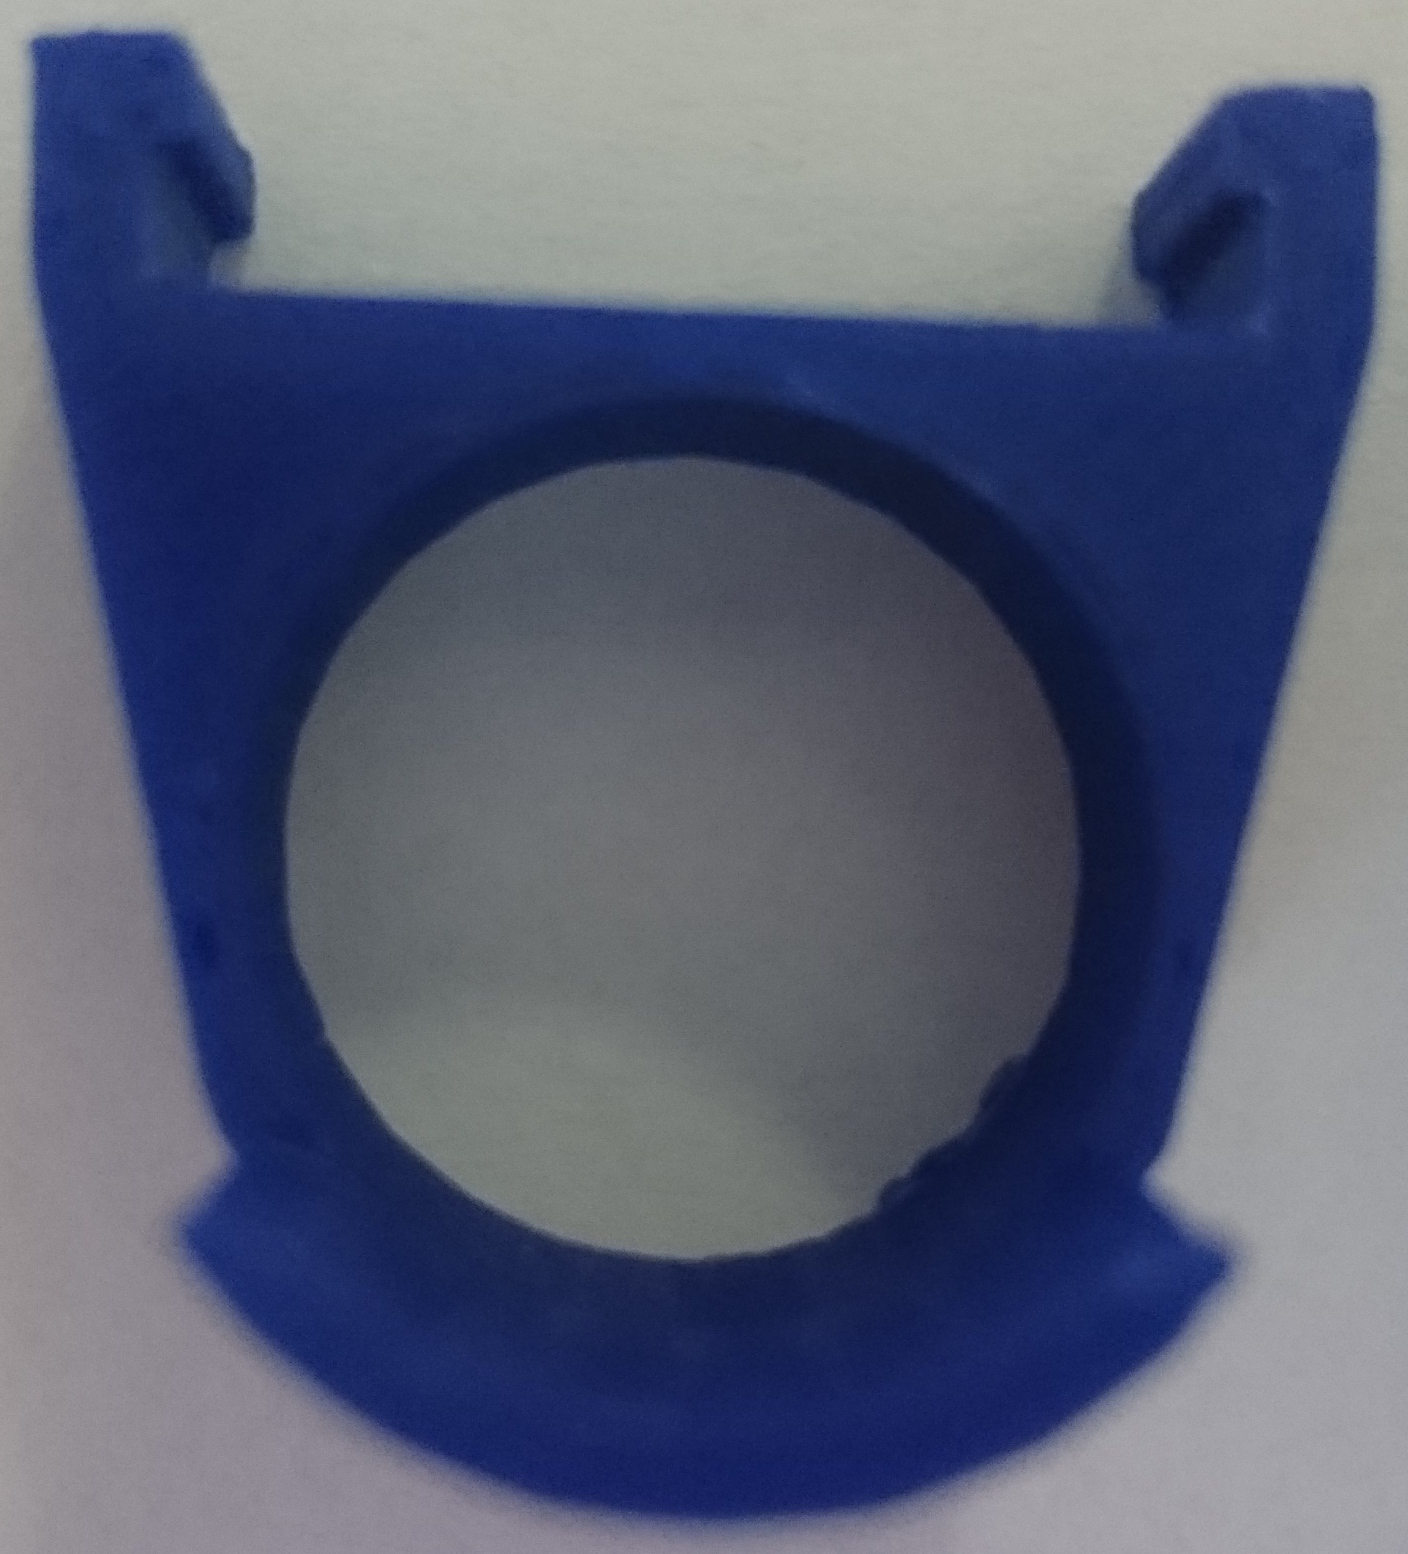
\includegraphics[width=0.12\textheight,height=0.12\textheight]{Images/0204_finger}
}
\subfloat[Thumb Ring x1]{
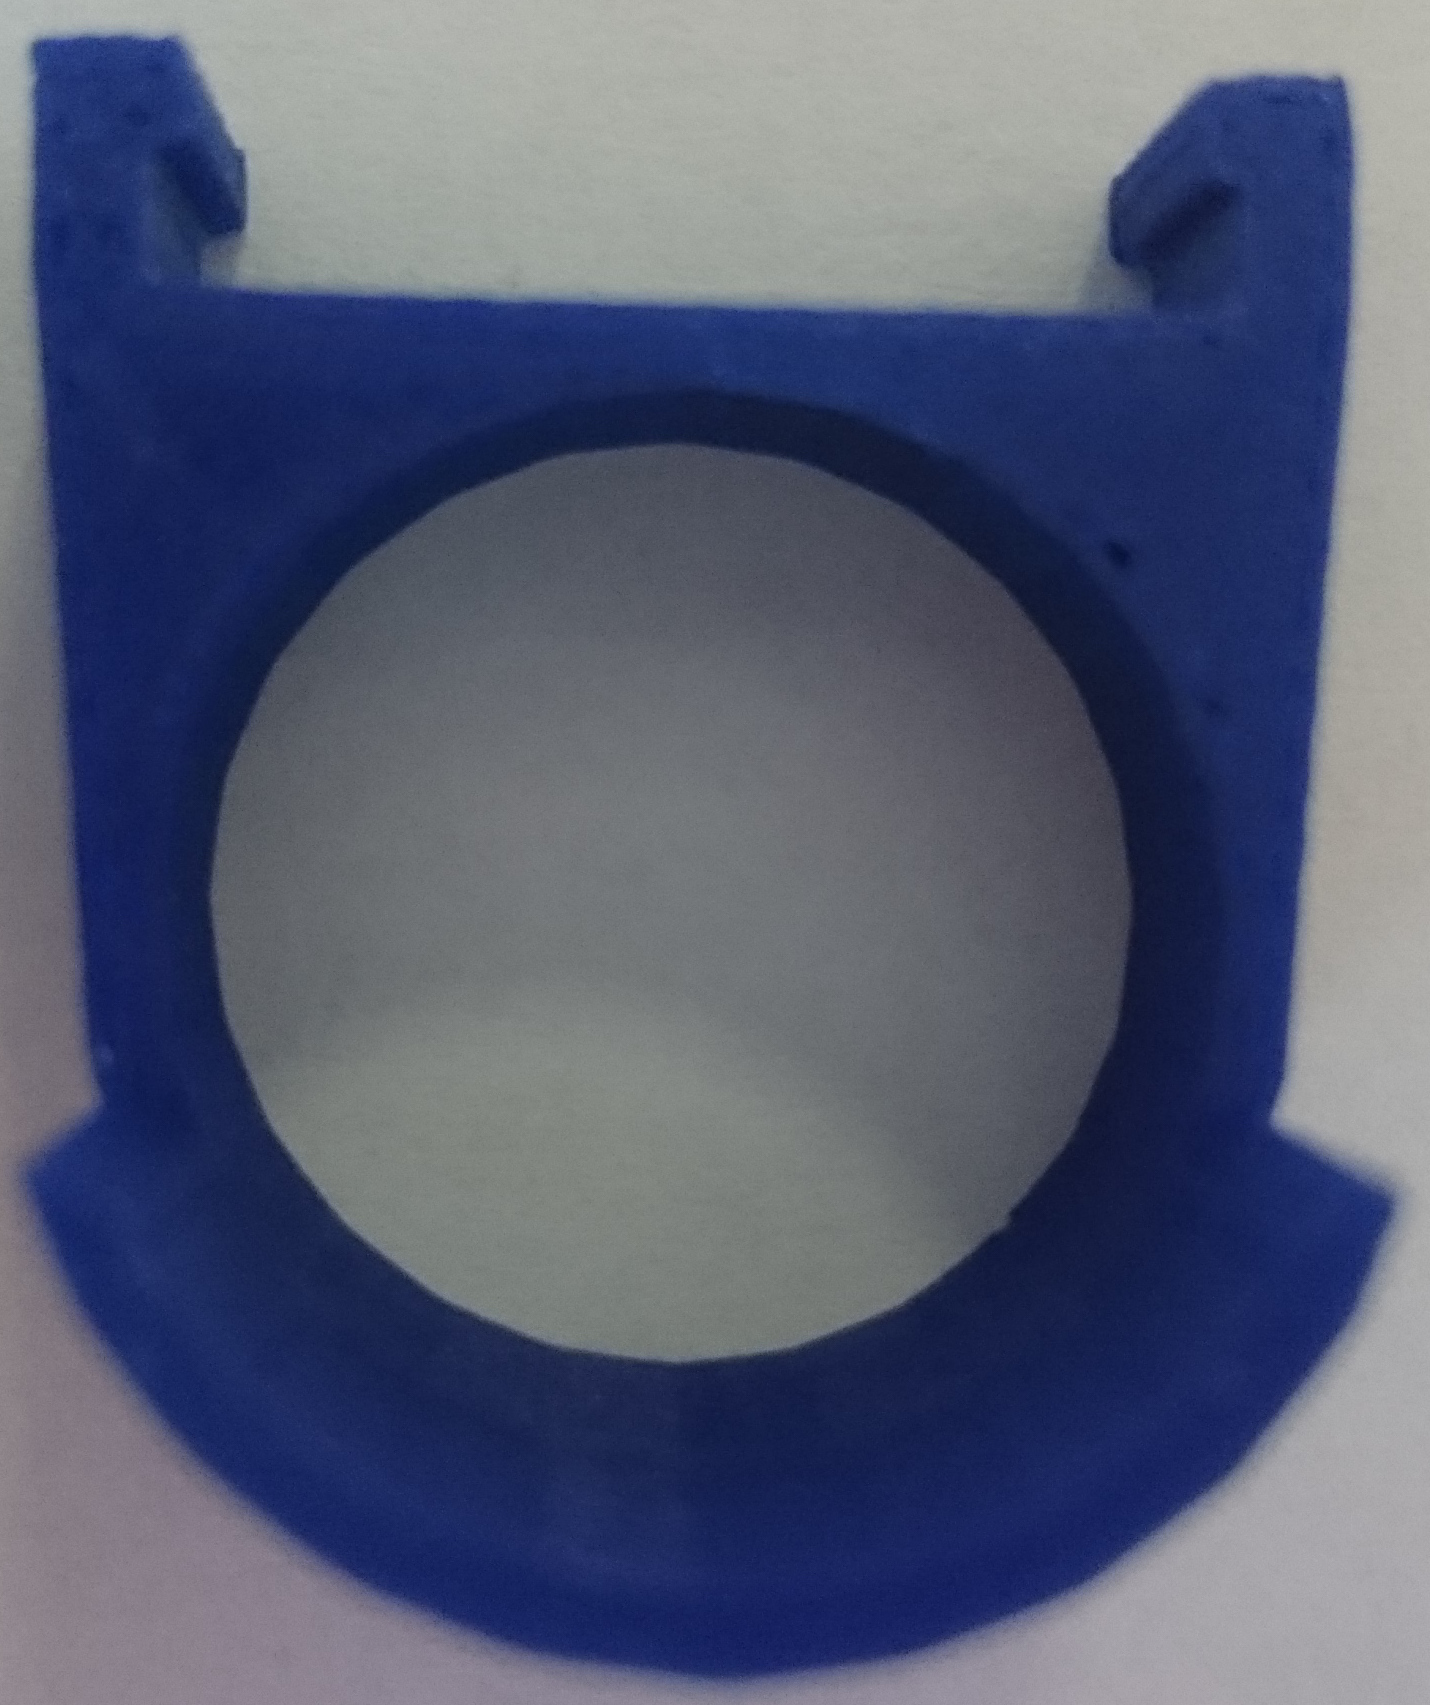
\includegraphics[width=0.12\textheight,height=0.12\textheight]{Images/0204_thumb}
}
\subfloat[Finger Board x3]{
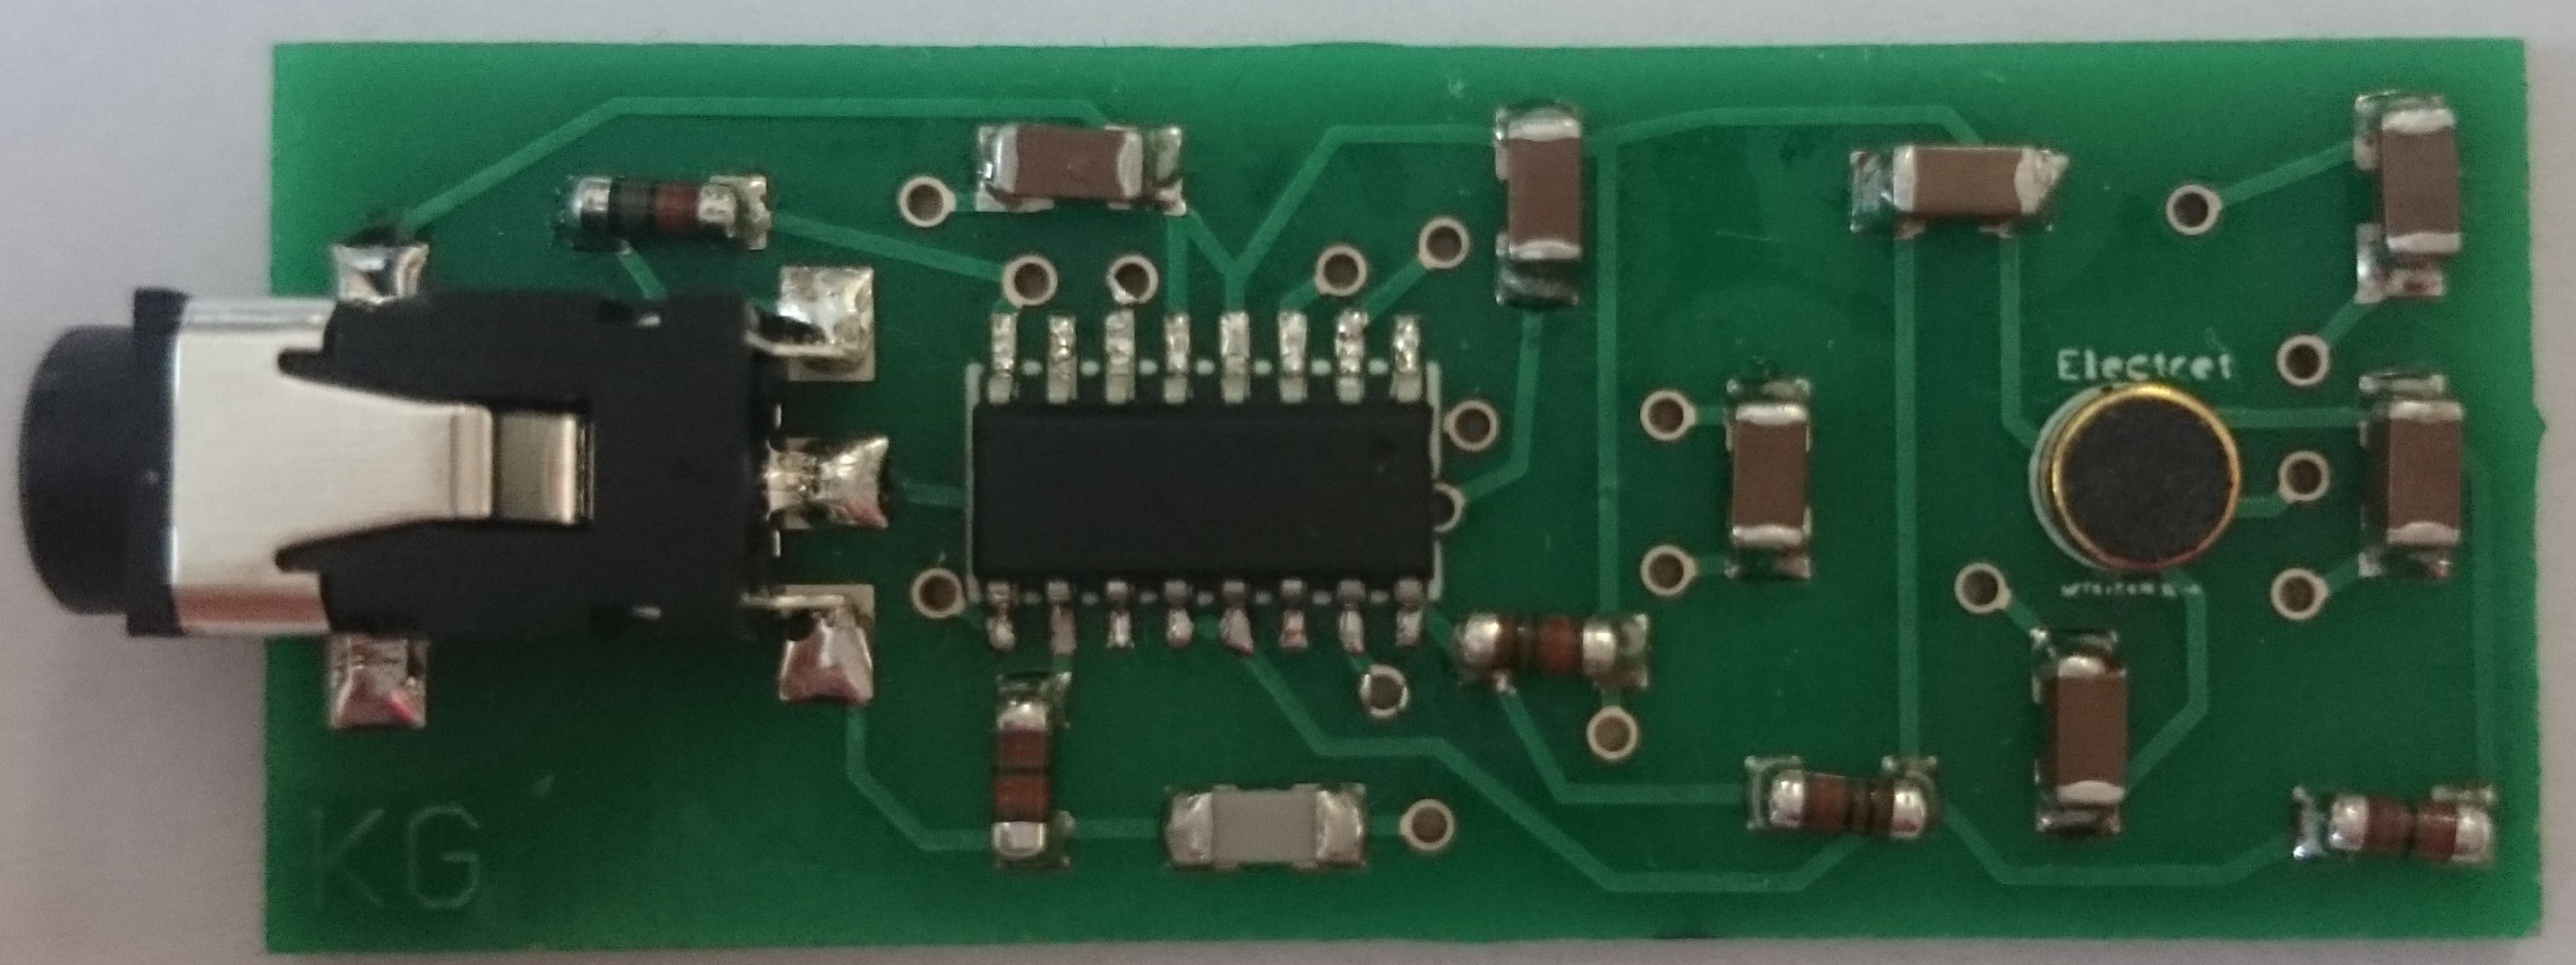
\includegraphics[width=0.36\textheight,height=0.12\textheight]{Images/0204_board}
}\\
\subfloat[Arduino Shield x1]{
\includegraphics[width=0.25\textheight,height=0.20\textheight]{Images/0204_shield}
}
\subfloat[Arduino Uno x1]{
\includegraphics[width=0.25\textheight,height=0.20\textheight]{Images/0204_arduino}
}\\
\subfloat[4-way Jack Cable x3]{
\includegraphics[width=0.25\textheight,height=0.20\textheight]{Images/0204_jackcable}
}
\subfloat[USB Type A/B Cable x1]{
\includegraphics[width=0.25\textheight,height=0.20\textheight]{Images/0204_usbcable}
}
\caption{List of hardware parts for PAWS instrument}
\label{fig:listofparts}
\end{figure}


\subsection{Setting Up the Hardware}

Firstly, the Finger Boards must be connected using the 4-way Jack Cables to the Arduino Shield. The Arduino can be slotted into the headers of the Arduino Uno to sit neatly on top, and the Uno can be connected via USB to a computer. The two Finger Rings and Thumb Ring can be worn on any hand, with the lip extrusions sitting comfortably under the fingertips, and the three Finger Boards can simply slide into the designated slots. Once this has been done, the instrument is ready to be used.

\subsection{Using the Software}

\begin{figure}[H]
\centering
\subfloat[Opening Screen]{
\includegraphics[scale = 0.25]{Images/paws_3_open}
\label{fig:paws_open}
}
\subfloat[Controls for 3 Finger Boards]{
\includegraphics[scale = 0.25]{Images/paws_3_connect}
\label{fig:paws_3controls}
}
\caption{PAWS Interface on Opening and Connecting to Arduino}

\end{figure}

Upon starting the PAWS application, the user is greeted with a thin purplish red line across the centre of the screen and a single 'Connect' button. When the 'Connect' button is pressed, provided that the Arduino has been connected to the correct USB port, the program will open three control interfaces for each of the three Finger Boards, as displayed in Figure~\ref{fig:paws_3controls}. A 'Disconnect' button will appear at the top of the program above the Board controls. 


The control interfaces, labelled 'One', 'Two', and 'Three, consist of buttons to select whether the user would like the corresponding Finger Board to operate in 'Voice' mode or 'Sample' mode. Each interface also hosts a blue dial to control the amplitude of the resulting signal from the respective Finger Board, and a large red dial below these controls the overall volume for the entire program.

When 'Voice' is selected for any Board, the sound captured by the Board's microphone will be played through the computer's output audio device. The thin line in the background of the display will also transform dynamically to display the waveform of the output sound for visual feedback.

\begin{figure}[H]
\centering
\subfloat[All Boards in 'Voice' mode]{
\includegraphics[scale = 0.25]{Images/paws_3_voice}
\label{fig:paws_open}
}
\subfloat[All Boards in 'Sample' mode]{
\includegraphics[scale = 0.25]{Images/paws_3_sample}
\label{fig:paws_3controls}
}
\caption{PAWS Interface in different modes}

\end{figure}

When 'Sample' is selected for any Board, a drop down list appears below the mode selection buttons to allow the user to choose a sample sound file. When the user taps a Finger Board against a surface, the program will play back the chosen sample sound file in response to the 'tap'. This mode allows for the user to convert a rhythm they play into a series of pre-recorded sounds, as determined by the sample sound files in the list. Since these sample files are in stereo, the thin line in the background of the display will transform into two separate waveforms: a red line to represent the left channel of the played sound, and a blue line to represent the right channel. When both of the stereo channels are identical, the two lines will converge and  return to its original purplish colour. 

The sample sound file can be freely chosen when in 'Sample' mode. When switching back to 'Voice' mode, the ability to choose a sample file will disappear from view. The modes can be switched between freely and at any time.

To shut down the program, the normal forms of quitting can be used (red button on top left, or the cmd+Q keyboard shortcut). The 'Disconnect' button can also be pressed before doing so, in which case all of the Board controls and overall volume control dial will disappear and the program will return to its starting screen. 





\subsection{Disconnecting the Hardware}

When the instrument has been finished with, the PAWS software must be closed first. Then the hardware is dismantled in the reverse order to setting it up: the usb cable is unplugged from the computer first, then from the Arduino. The Arduino Shield may be kept connected to the Arduino Uno but the Finger Boards must be disconnected from the Uno and all cable rolled away neatly for storage. The Finger Boards may be removed from the Ring housings if necessary. 

The order of disassembly is important as the Interface will crash if the Arduino is unplugged during run-time, and the Arduino must be disconnected from the computer before removing the Finger Boards to ensure that there is no power surging through the cables during this process. 


\newpage


%%%%%%%%%%%%%%%%%%%%%%%%%%%%%%%%%%%%%%%%%%%%%%%%%%%%%%%%%%%%%%%%%%%%%%%%%%%%%%%%%%%%%%%%%%%%%%%%%%%%%%%%%%%%%%%%%%%%%%%%%%%%%%%%%%%%%%%%%%%%%%%%%%%%%%%%%%%%%%%%%%%%%%%%%%%%%%%%%%%% 
\newpage
%%%%%%%%%%%%%%%%%%%%%%%%%%%%%%%%%%%%%%%%%%%%%
% !TEX root = /Users/kartikgohil/Documents/Imperial/Year4/Project/Docs/Final_Report/report_tex/main.tex

\begin{thebibliography}{99}

\bibitem{mimu}
    Mi.Mu Gloves. \emph{Mi.Mu: About}. [Online] Available from: http://mimugloves.bigcartel.com/mi-mu-bio [Accessed 24 Jan 2015].
    
\bibitem{mimugloves}
    Mi.Mu Gloves. \emph{Mi.Mu Collaborator Gloves}. [Online] Available from:  http://mimugloves.bigcartel.com/
    product/collaborator-gloves [Accessed 25 Jan 2015].
    
\bibitem{drumpants}
    DrumPants Inc. \emph{DrumPants}. [Online] Available from: http://www.drumpants.com/ [Accessed 24 Jan 2015].

\bibitem{drumpantsprice}
    DrumPants Inc. \emph{DrumPants}. [Online] Available from: https://legacy.trycelery.com/shop/drumpants [Accessed 25 Jan 2015].

\bibitem{gesturering}
    Logbar Inc. \emph{Ring}. [Online] Available from: http://logbar.jp/ring/en [Accessed 25 Jan 2015].
    

\bibitem{arduinopic}
    Arduino. \emph{Arduino Uno}. [Online] Available from: http://arduino.cc/en/main/arduinoBoardUno [Accessed 28 Jan 2015].
    
\bibitem{hc06ebay}
    Ebay. \emph{5V JY-MCU HC-06 V1.04 Bluetooth Transeiver RF Module Serial Port 51 AVR MCU ARM} [Online] http://www.ebay.com/itm/5V-JY-MCU-HC-06-V1-04-Bluetooth-Transeiver-RF-Module-Serial-Port-51-AVR-MCU-ARM-/261121350024 [Accessed 28 Jan 2015].
    
\bibitem{arduinosite}
    Arduino. \emph{Arduino}. [Online] Available from: http://arduino.cc [Accessed 28 Jan 2015].

\bibitem{pyolibrary}
    Olivier B\'{e}langer, Ajax Sound Studio. \emph{PyO 0.7.3 Documentation > API Documentation > Classes By Category}. [Online] Available from: http://ajaxsoundstudio.com/pyodoc/api/classes/index.html [Accessed 28 Jan 2015].


\bibitem{kingstatedatasheet}
    Premier Farnell plc. \emph{Specification for Approval - KINGSTATE, Electret Condenser Microphone, KEEG1542PBL-A}. [Online] Available from: http://www.farnell.com/datasheets/1780663.pdf [Accessed 12 Jan 2015].


\bibitem{queuelist}

    Efstathios Chatzikyriakidis. \emph{QueueList Library for Arduino}. [Online] Available from: http://playground.arduino.cc/Code/QueueList [Accessed 17 Jan 2015].

\bibitem{queuearray}

    Efstathios Chatzikyriakidis. \emph{QueueArray Library for Arduino}. [Online] Available from: http://playground.arduino.cc/Code/QueueArray [Accessed 17 Jan 2015].

\bibitem{pyserial}
    Chris Liechti, SourceForge. \emph{Welcome to pySerial's documentation}. [Online] Available from: http://pyserial.sourceforge.net [Accessed 29 Jan 2015].

\bibitem{pydub}
    Jiaaro. \emph{Pydub by jiaaro}. [Online] Avaliable from: http://pydub.com [Accessed 1 Feb 2015].

\bibitem{pyaudio}
    Hubert Pham. \emph{PyAudio 0.2.8 documentation > PyAudio Documentation}. [Online] Available from: http://people.csail.mit.edu/hubert/pyaudio/docs/ [Accessed 1 Feb 2015].
    
    
\bibitem{pyasparticle}
    John Glover, Victor Lazzarini, Joseph Timoney. Python For Audio Signal Processing. The Sound and Digital Music Research Group. [Online] 2011. Available from: http://lac.linuxaudio.org/2011/papers/40.pdf [Accessed 1 Feb 2015].

\bibitem{arduinobluetooth}
    techbitar, Instructables. \emph{Cheap 2-Way Bluetooth Connection Between Arduino and PC}. [Online] Available from: http://www.instructables.com/id/Cheap-2-Way-Bluetooth-Connection-Between-Arduino-a/ [Accessed 1 Feb 2015].

\bibitem{rtdsppaper}
    Ferruccio Bettarelli, Emanuele Ciavattini, Ariano Lattanzi, Francesco Piazza, Stefano Squartini, Diego Zallocco. NU-Tech: Implementing DSP Algorithms in a Plug-in Based Software Platform for Real time Audio Applications. [Online] 2005. Available from: http://www.aes.org/e-lib/browse.cfm?elib=13105\&rndx=768511 [Accessed 2 Feb 2015].

\bibitem{spikedetection}
    Scott B. Wilson, Ronald Emerson. Spike detection: a review and comparison of algorithms. \emph{Clinical Neurophysiology}. Volume 113, Issue 12, Pages 1873-1881. [Online] 2002. Available from: http://dx.doi.org/10.1016/S1388-2457(02)00297-3 [Accessed 2 Feb 2015].
    
\bibitem{transientdetectionpaper}
    V. Datta, G.V. Anand. Transient detection in non-Gaussian noise by wavelet packet transform. [Online] 2010. Available from: doi:10.1109/SPCOM.2010.5560494 [Accessed 2 Feb 2015].

\bibitem{wxpython}
Julian Smart, Vadim Zeitlin, Robin Dunn, Stefan Csomor, Bryan Petty, Francesco Montorsi, Robert Roebling et al. \textit{wxWidgets: Documentation}. [Online] 6 Oct 2014. Available from: http://www.wxpython.org/onlinedocs.php [Accessed 10 Jun 2015].

\bibitem{pwmanalog}
Ryan Metivier. Allegro MicroSystems, LLC. \textit{Method for Converting a PWM Output to an Analog Output When Using Hall Effect Sensor ICs}. [Online] Available from: http://www.allegromicro.com/en/Design-Center/Technical-Documents/Hall-Effect-Sensor-IC-Publications/Method-for-Converting-a-PWM-Output-to-an-Analog-Output-When-Using-Hall-Effect-Sensor-ICs.aspx [Accessed 10 Jun 2015].

\bibitem{analogread}
Arduino. \textit{analogRead()}. [Online] 2015. Available from: http://www.arduino.cc/en/Reference/AnalogRead [Accessed 10 Jun 2015].

\bibitem{juce}
Roli Ltd. \textit{JUCE}. [Online] Available from: https://www.juce.com [Accessed 10 Jun 2015].

\bibitem{introjucer}
Roli Ltd. \textit{The Introjucer}. [Online] Available from: http://www.juce.com/learn/introjucer  [Accessed 10 Jun 2015].

\bibitem{pthread}
Blaise Barney, Lawrence Livermore National Laboratory. \textit{POSIX Threads Programming}. [Online] 6 Apr 2015. Available from: https://computing.llnl.gov/tutorials/pthreads/ [Accessed 10 Jun 2015].

\bibitem{termios}
Wikibooks. \textit{Serial Programming/termios}. [Online] 25 Apr 2015. Available from: http://en.wikibooks.org/wiki/Serial\_Programming/termios [Accessed 10 Jun 2015].

\bibitem{eagle}
Cadsoft \textit{About EAGLE PCB Design Software}. [Online] 2011. Available from: http://www.cadsoftusa.com/eagle-pcb-design-software/about-eagle/ [Accessed 10 Jun 2015].

\bibitem{sketchup}
Trimble Navigation Limited. \textit{SketchUp: The easiest way to draw in 3D}. [Online] 2013. Available from: http://www.sketchup.com [Accessed 10 Jun 2015].

\bibitem{cura}
Ultimaker. \textit{Cura: You And Cura Made For Each Other}. [Online] 2015. Available from: https://ultimaker.com/en/products/software [Accessed 10 Jun 2015].

\bibitem{ultimaker}
Ultimaker. \textit{Ultimaker 2 Family: Our family made to make you smile}. [Online] 2015. Available from: https://ultimaker.com/en/products/ultimaker-2-family [Accessed 10 Jun 2015].

\bibitem{overlap}
Ali Daher, El Houssa�n Baghious, Gilles Burel, Senior Member, IEEE, and Emanuel Radoi. Overlap-Save and Overlap-Add Filters: Optimal Design and Comparison. \textit{IEEE Transactions on Signal Processing} Volume 58, No. 6. [Online] June 2010. Available from: http://ieeexplore.ieee.org/stamp/stamp.jsp?arnumber=5419990 [Accessed 16 Jun].

\bibitem{thermalnoise}


\bibitem{groundplane}


\bibitem{oversampling}


\bibitem{codewords}



\bibitem{ts7001}
Touchstone Semiconductor Inc. \textit{TS7001: A Micropower, 2-channel, 187.5-ksps, Serial-Output 12-bit SAR ADC}. [Online] Available from: http://www.farnell.com/datasheets/1774447.pdf [Accessed 9 Jun 2015]

\bibitem{microusbconnector}
Hirose Electric Co., Ltd. \textit{?Micro-USB connectors meeting USB 2.0 Standard: ZX Series}. [Online] Available from: http://docs-europe.electrocomponents.com/webdocs/1363/0900766b81363588.pdf [Accessed 9 Jun 2015]

\bibitem{microusbcable}
Roline. \textit{ROLINE USB 2.0 Cable, USB Type A M - Micro USB B M 1.8 m}. [Online] Available from: http://docs-europe.electrocomponents.com/webdocs/125b/0900766b8125b918.pdf [Accessed 9 Jun 2015]

\end{thebibliography} 
 
\newpage
%%%%%%%%%%%%%%%%%%%%%%%%%%%%%%%%%%%%%%%%%%%%%
% !TEX root = /Users/kartikgohil/Documents/Imperial/Year4/Project/Docs/Final_Report/report_tex/main.tex
\section{Appendices}
\appendix

\section{Circuit Diagrams} \label{Circuit Diagrams}


\subsection{Circuit Diagram for HC-06 to Arduino Connection}
\label{arduinobluetooth}
\begin{figure}[H]
\centering
\includegraphics[scale = 1]{Images/arduinobluetooth}
\caption*{Image Available from Reference~\cite{arduinobluetooth}}
\end{figure}

\subsection{Circuit Diagram for Prototype 0.2.03 - Finger Board}
\label{fingerboardsch}
\begin{figure}[H]
\centering
\includegraphics[scale = 1]{Images/mic_schematic_01}
\end{figure}

\subsection{Circuit Diagram for Prototype 0.2.03 - Arduino Shield}
\label{ardshieldsch}
\begin{figure}[H]
\centering
\includegraphics[scale = 1]{Images/ard_schematic_01}
\end{figure}



\section{Flow Diagrams} \label{Flow Diagrams}

\subsection{Flow Diagram for Microcontroller Program, Prototype 0.1.01}
\label{mcflow}
\begin{figure}[H]
\centering
\includegraphics[scale = 1]{Images/mc0101}
\end{figure}


\newpage
\subsection{Flow Diagram for Interface Program, Prototype 0.1.01}
\label{interfaceflow}
\begin{figure}[H]
\centering
\subfloat[Voice Function Program]{
\includegraphics[scale = 1]{Images/interfacevoiceflow}
}
\hspace{72pt}
\subfloat[Sample Function Program]{
\includegraphics[scale = 1]{Images/interfacesampleflow}
}
\end{figure}

\subsection{Flow Diagram for Interface Program, Prototype 0.1.02}
\label{pyblue_flow}
\begin{figure}[H]
\centering
\includegraphics[scale = 0.7]{Images/PyFlow}
\end{figure}

\subsection{Flow Diagram for Interface Program, Prototype 0.2.01}
\label{juceflow}
\begin{figure}[H]
\centering
\includegraphics[scale=0.7]{Images/JuceFlow}\\
Function Diagram of Audio Transfer between storage buffers for each connected Board and the audio device.
\end{figure}


\section{PCB Design}

\subsection{Finger Board}
\label{fingerboardpcb}
\begin{figure}[H]
\centering
\includegraphics[scale = 2]{Images/mic_pcb_02}
\\ Dimensions: 49.51 x 19.99 mm
\end{figure}

\subsection{Arduino Shield Version 1}
\label{ardshieldpcb}
\begin{figure}[H]
\centering
\includegraphics[scale = 1.5]{Images/ard_pcb_01}
\\ Dimensions: 68.58 x 53.34 x 2.5mm
\end{figure}

\subsection{Arduino Shield Version 2}
\label{ardshieldpcb2}
\begin{figure}[H]
\centering
\includegraphics[scale = 1.5]{Images/ard_pcb_02}
\\ Dimensions: 68.58 x 53.34 x 2.5mm
\end{figure}


\section{GitHub Repository}

Documentation for this project including all versions of code, 3D models, circuit designs, report drafts, Matlab simulations, etc. can be found in the following GitHub Repository: https://github.com/kartikg33/imp\_fyp\_2015





\end{document}